% **************************************************
% Macro specifiche per il documento corrente
% **************************************************
% Nome
\newcommand{\docName}{Specifica tecnica}
% Nome file
\newcommand{\docFileName}{specifica\_tecnica.1.0.pdf}
% Versione
\newcommand{\docVers}{1.0}
% Data creazione
\newcommand{\creationDate}{2013-01-23}
% Data ultima modifica
\newcommand{\modificationDate}{2013-01-30}
% Stato in {Approvato, Non approvato}
\newcommand{\docState}{Approvato}
% Uso in {Interno, Esterno}
\newcommand{\docUsage}{Esterno}
% Destinatari da specificare come nome1\\ &nome2\\ ecc.
\newcommand{\docDistributionList}{Prof. Tullio Vardanega\\&Prof. Riccardo Cardin\\&Dott. Gregorio Piccoli\\&Team SoftwareSynthesis}
% Redattori da specificare come nome1\\ &nome2\\ ecc.
\newcommand{\docAuthors}{Diego Beraldin\\&Elena Zecchinato\\&Marco Schivo}
% Approvato da
\newcommand{\approvedBy}{Riccardo Tresoldi}
% Verificatori
\newcommand{\verifiedBy}{Andrea Meneghinello\\&Stefano Farronato}
% Perscorso (relativo o assoluto) che punta alla directory contenente shared/
% come sua sottodirectory (per comodità chiamiamola 'doc root').
\newcommand{\docRoot}{..}
% definire se si vuole l'indice delle tabelle
\def\INDICETABELLE{false}
% definire se si vuole l'indice delle figure
\def\INDICEFIGURE{true}

% importa il preambolo condiviso da tutti i documenti
% shared/preamble.tex
%
% Questo documento contiene la parte del preambolo condivisa e viene pertanto
% richiamato nel 'master' di tutti i documenti di progetto.  Al suo interno
% contiene le inclusioni (e le configurazioni) di tutti i package richiesti per
% la compilazione dei documenti, le macro di carattere generale e la definizione
% degli stili di pagina.

\documentclass[a4paper,10pt,openright]{article}

% **************************************************
% Macro generiche
% **************************************************
\newcommand{\team}{Software Synthesis}                    % chi siamo
\newcommand{\email}{software.synthesis@gmail.com}         % e-mail
\newcommand{\caName}{}                                    % titolo capitolato
\newcommand{\caDescr}{}                                   % descrizione
\newcommand{\inglese}[1]{\textit{#1}}

% **************************************************
% Codifica e lingua dei documenti
% **************************************************
\usepackage[utf8x]{inputenc}                              % codifica caratteri dei documenti sorgenti
\usepackage[english,italian]{babel}                       % localizzazione ai fini di sillabazione e cross-references
\usepackage[T1]{fontenc}                                  % codifica font di output

% **************************************************
% Definizione geometria della pagina
% **************************************************
\usepackage[a4paper,head=4cm,top=4.5cm,bottom=3cm,left=3cm,right=3cm,bindingoffset=5mm]{geometry}

% *************************************************
% Intestazioni e piè di pagina personalizzati
% *************************************************
\usepackage{fancyhdr}
% stile normale
\fancypagestyle{normal}{
\fancyhead{}                                              % intestazione
\fancyhead[RE,RO]{
\begin{picture}(0,0)
  \put(-410,0){
\includegraphics[width=1.02\textwidth]{header_logo}}
  \put(-410,10){\sffamily\large\leftmark}
\end{picture}
\vspace{-4pt}
}
\renewcommand{\headrulewidth}{.4pt}                       % riga sotto l'intestazione
\cfoot{}                                                  % piè di pagina
\fancyfoot[RO,LE]{\sffamily
  pag.~\thepage{} di \pageref{LastPage}}                  % a dx nelle pag. dispari e a sx in quelle pari
\fancyfoot[RE,LO]{\sffamily\docFileName{} -- v.\docVers}
\renewcommand{\footrulewidth}{.4pt}                       % riga sopra il piè di pagina
}
% stile per gli indici
\fancypagestyle{toc}{
\fancyhead{}                                              % intestazione
\fancyhead[RE,RO]{
\begin{picture}(0,0)
  \put(-410,0){
\includegraphics[width=1.02\textwidth]{header_logo}}
\end{picture}
}
\renewcommand{\headrule}{}                                % nessuna riga sotto l'intestazione
\cfoot{}                                                  % piè di pagina
\fancyfoot[RO,LE]{\sffamily\thepage{}}                    % a dx nelle pag. dispari e a sx in quelle pari
\fancyfoot[RE,LO]{\sffamily\docFileName{} -- v.\docVers}
\renewcommand{\footrulewidth}{.4pt}                       % riga sopra il piè di pagina
}

\pagestyle{fancy}                                         % premetto: non so usare bene le marche:
\renewcommand{\sectionmark}[1]{\markboth{#1}{#1}}         % se qualcuno ha idee migliori si faccia avanti!

% **************************************************
% Tabelle
% **************************************************
\usepackage{tabularx}                                     % tabelle di larghezza fissa con una o più colonne variabili
\usepackage{multirow}                                     % colonne con colonne che si estendono per più righe
\usepackage{booktabs}                                     % per inserire l'ambiente table e le righe orizz. nelle tabelle
\usepackage{longtable}			                          % tabelle oltre i limiti di pagina

% **************************************************
% Cross-references e collegamenti ipertestuali
% **************************************************
\usepackage[hidelinks]{hyperref}
\hypersetup{%
  colorlinks=false, linktocpage=false, pdfborder={0,0,0}, pdfstartpage=3, pdfstartview=FitV,%
  urlcolor=Cyan, linkcolor=Cyan, citecolor=Black, %pagecolor=Black,%
  pdftitle={\docName}, pdfauthor={\team}, pdfsubject={}, pdfkeywords={},%
  pdfcreator={pdflatex}, pdfproducer={pdflatex with hyperref package}%
}

% **************************************************
% Immagini e grafica
% **************************************************
\usepackage{graphicx}                                     % supporto ad aspetti avanzati delle immagini
\graphicspath{{\docRoot/pics/}}                           % percorso contenente tutti i file immagini
\usepackage{color}                                        % permette di colorare facilmente il testo

% **************************************************
% Altri pacchetti opzionali
% **************************************************     
\usepackage{lastpage}                                     % per sapere il numero totale di pagine
\usepackage{lipsum}                                       % genera "dummy text" per prove di impaginazione
\usepackage{eurosym}                                      % per il simbolo dell'euro usare \EUR{x} dove x è l'importo


% Fine del preambolo e inizio del documento
\begin{document}

% Inclusione della prima pagina
% shared/firstpage.tex
%
% Questo documento definisce il contenuto della prima pagina, che si suppone
% essere uguale in tutti i documenti.  Oltre al logo e al titolo, la prima
% pagina contiene i metadati relativi al documento in cui viene inclusa.


% rimuove intestazioni e piè di pagina
\pagestyle{empty}

\begin{center}

% logo del gruppo

\includegraphics[width=1.5\textwidth]{logo}

\vspace{1in}

% titolo del documento
{\Huge\bfseries \docName}

\vspace{1in}

% tabella riepilogativa
\begin{tabularx}{.7\textwidth}{>{\bfseries\sffamily}l>{\sffamily}l}
\toprule
\multicolumn{2}{>{\sffamily}c}{Informazioni sul documento}\\
\midrule
Nome file:            & \docFileName\\
Versione:             & \docVers\\
Data creazione:       & \creationDate\\
Data ultima modifica: & \modificationDate\\
Stato:                & \docState\\
Uso:                  & \docUsage\\
Redattori:            & \docAuthors\\
Approvato da:         & \approvedBy\\
Verificatori:         & \verifiedBy\\
\bottomrule
\end{tabularx}

\end{center}

\newpage


%---------------------------RUOLI----------------------------
%FASE 1:
%Progettisti: TRES, STEFANO, SCHIVO;
%FASE 2:
%Progettisti: DIEGO, ELENA, RIZZI

%Verificatore: Andrea Meneghinello
%Responsabile finale TRES
%------------------------------------------------------------

% Storico delle modifiche
\section*{Storia delle modifiche}
\begin{center}
\begin{longtable}{lp{.32\textwidth}lll}
\toprule
Versione & Descrizione intervento & Membro & Ruolo & Data\\
\midrule % inserire qui il contenuto della tabella
1.1 & Modifica architettura del database & Elena Zecchinato & Progettista & 2012-02-08\\
1.0 & Approvazione documento &Riccardo Tresoldi & Responsabile & 2012-01-30\\
0.19 & Correzione errori ortografici e di forma presenti nel documento in base alle segnalazioni del verificatore&Marco Schivo & Progettista & 2013-01-29\\
0.18 & Correzione diagrammi presenti nel documento in base alle segnalazioni del verificatore&Elena Zecchinato & Progettista & 2013-01-29\\
0.17 & Verifica lessico ortografica del documento & Andrea Meneghinello & Verificatore & 2013-01-28\\
0.16 & Verifica correttezza e corrispondenza dei diagrammi presenti nel documento & Stefano Farronato & Verificatore & 2013-01-27\\
0.15 & Inserimento tabelle di tracciamento prodotte nel capitolo 12&Diego Beraldin & Progettista & 2013-01-28\\
0.14 & Inserimento diagrammi delle attività e dei package prodotti nel capitolo 11&Diego Beraldin & Progettista & 2013-01-28\\
0.13 & Inserimento diagrammi delle classi nel capitolo 6, 7, 8, 9&Marco Schivo & Progettista & 2013-01-28\\
0.12 & Inserimento diagrammi relativi ai design pattern evidenziati&Marco Schivo & Progettista & 2013-01-28\\
0.11 & Inizio stesura capitolo relativo alla descrizione delle classi&Diego Beraldin & Progettista & 2013-01-27\\
0.10 & Stesura della sezione relativa all'architettura mytalk.clientview stilando i componenti evidenziati&Elena Zecchinato & Progettista & 2013-01-27\\
0.9 & Stesura della sezione relativa all'architettura mytalk.clientpresenter stilando i componenti evidenziati&Marco Schivo & Progettista & 2013-01-27\\
0.8 & Stesura della sezione relativa all'architettura mytalk.server stilando i componenti evidenziati&Marco Schivo & Progettista & 2013-01-26\\
0.7 & Stesura della sezione relativa alla progettazione logica &Diego Beraldin  & Progettista & 2013-01-26\\
0.6 & Completata la sezione relativa alla progettazione concettuale &Elena Zecchinato & Progettista & 2013-01-25\\
0.5 & Inizio stesura della sezione relativa alla progettazione concettuale con classi evidenziate in fase di progettazione &Elena Zecchinato& Progettista & 2013-01-24\\
0.4 & Descrizione dei design pattern evidenziati nella fase di progettazione. &Diego Beraldin & Progettista & 2013-01-24\\
0.3 & Aggiunto capitolo relativo agli strumenti utilizzati.& Marco Schivo & Progettista & 2013-01-23\\
0.2 & Stesura dell'introduzione ai design pattern. Stesura dell'introduzione ai tracciamenti. &Elena Zecchinato & Progettista & 2013-01-23\\
0.1 & Creazione del documento e stesura della sezione ``Introduzione''. &Diego Beraldin & Progettista & 2013-01-23\\
\bottomrule
\end{longtable}
\end{center}
\newpage

% inclusione dell'indice
% shared/toc.tex
%
% Questo file contiene le istruzioni che generano l'indice o gli indici del
% documento (utile nel caso in cui decidessimo di avere anche un indice delle
% tabelle e/o un indice delle figure).

\pagestyle{toc}
\pagenumbering{roman}

\tableofcontents

\newpage


% Alcuni aggiustamenti per le pagine
\pagenumbering{arabic}
\setcounter{page}{1}
\pagestyle{normal}

% Qui ha inizio il documento vero e proprio...
\newpage

\section{Introduzione}
\subsection{Scopo del prodotto}
\purpose

\subsection{Scopo del documento}
Il presente documento è stato redatto al fine di produrre le specifiche sulla progettazione ad alto livello, del prodotto \caName. A tal fine il documento presenterà:
\begin{itemize}
    \item una descrizione degli strumenti e dei \underline{framework} su cui si basa l'architettura;
	\item un elenco con le specifiche dei \underline{design pattern} utilizzati;
	\item l'architettura di alto livello del sistema;
	\item una descrizione dettagliata dei componenti rilevati in fase di progettazione indicando relativamente a ciascuno di essi il tipo, la funzione e l'obiettivo;
	\item i diagrammi UML per definire i flussi principali di controllo dell'applicativo;
	\item il tracciamento dei requisiti e dei componenti, negli schemi: requisiti-componenti e componenti-requisiti;
	\item il tracciamento di componenti e \underline{design pattern};
	\item il tracciamento di classi e componenti.
\end{itemize}

\subsection{Glossario}
\glossaryIntro

\clearpage
\section{Riferimenti}

\subsection{Normativi}
\begin{itemize}
\item[] \textit{piano\_di\_qualifica.2.0.pdf} allegato.
\item[] \textit{norme\_di\_progetto.2.0.pdf} allegato.
\item[] \textit{analisi\_dei\_requisiti.2.0.pdf} allegato
\end{itemize}

\subsection{Informativi}
\begin{itemize}
\item[] Capitolato d'appalto: \caName{}, v1.0, redatto e rilasciato dal proponente Zucchetti s.r.l. reperibile all'indirizzo \url{http://www.math.unipd.it/~tullio/IS-1/2012/Progetto/C1.pdf};
\item[] testo di consultazione: \textit{Software Engineering (8th edition) Ian Sommerville, Pearson Education | Addison Wesley};
\item[] manuale all'utilizzo dei design pattens: \textit{Design Patterns, Elementi per il riuso di software a oggetti -- (1/Ed. italiana) Eric Gamma, Richard Helm, Ralph Johnson, John Vlissides, Pearson Education};
\item[] manuale di basi di dati: \textit{Sistemi di basi di dati-fondamenti} -- (6° edizione) Ramez Elmasri / Shamkant B. Navathe
\item[] \textit{glossario.2.0.pdf} allegato.
\end{itemize}
\clearpage

\section{Strumenti utilizzati}
\subsection{Java}
L'utilizzo del linguaggio \underline{Java} è richiesto dal proponente esclusivamente per la realizzazione della componente \underline{server}.

\subsubsection*{Vantaggi}
\begin{itemize}
\item[-] è un linguaggio predisposto nativamente alla gestione parallela di thread e questo applicato ad un \underline{server} dà la possibilità di gestire parallelamente richieste da parte di più utenti allo stesso tempo;
\item[-] essendo un linguaggio orientato agli oggetti e fortemente tipizzato si presta all'applicazione di \underline{design pattern} e alla costruzione di un'architettura robusta, fortemente modulare e al contempo flessibile, in accordo con i principi del paradigma di programmazione OO;
\item[-] permette la generazione automatica della documentazione con l'ausilio di JavaDoc;
\item[-] garantisce la portabilità del codice (a livello di bytecode), l'indipendenza dalla piattaforma fisica di esecuzione grazie alla JVM e l'integrazione nell'ambiente di esecuzione del proponente (\underline{TomCat}).
\end{itemize}

\subsection{Hibernate}
Hibernate è un \underline{framework} \underline{Java} utilizzato per facilitare l'utilizzo di un \underline{database} da parte del \underline{server} realizzando la mappatura fra oggetti intesi in senso OOP ed ennuple del modello relazionale (Object-Relational Mapping).

\subsubsection*{Vantaggi}
\begin{itemize}
\item[-] Hibernate permette di utilizzare le tabelle di un \underline{database} relazionale come se fossero degli oggetti mappando il \underline{database} su di opportune classi strutturate ad-hoc svincolando la gestione della persistenza dei dati dalla logica di business;
\item[-] con questo \underline{framework} \underline{Java} riesce a lavorare su un \underline{database} rendendo trasparenti al programmatore le vere e proprie query e mostrando esclusivamente classi e metodi;
\item[-] essendo rilasciato sotto licenza LGPL può essere utilizzato senza restrizioni (copyleft) e vincoli di licenza delle opere derivate. 
\end{itemize}
\clearpage

\section{Design Pattern utilizzati}
In questa sezione discuteremo i \underline{design pattern} utilizzati nella progettazione dei componenti architetturali. Ogni \underline{design pattern} sarà proposto con la seguente forma:
\begin{itemize}
	\item \textbf{Scopo}: verrà proposto lo scopo generico del pattern, al fine di evidenziare subito la sua utilità.
	\item \textbf{Diagramma esemplificativo}: si riporterà lo schema UML, rappresentante un implementazione generica del \underline{design pattern} in esame.
	\item \textbf{Vantaggi derivanti}: si darà un elenco dei vantaggi apportati dall'utilizzo del pattern, in particolare sotto il profilo della manutenzione e del riuso del codice.
	\item \textbf{Componenti che lo implementano}: infine verranno elencati i componenti dell'architettura di sistema, che implementano il pattern descritto.
\end{itemize}

Per una visione d'insieme dei componenti utilizzati da un pattern, e dei pattern utilizzati da un componente, rimandiamo alle sottosezioni ``Tracciamenti Componenti-Design Pattern'' e ``Tracciamenti Design Pattern-Componenti'' della sezione \vref{sec:tracciamenti}.

\subsection{Composite}

\subsubsection{Scopo}
Il pattern Composite ha lo scopo di comporre oggetti in strutture ad albero al fine di rappresentare gerarchie parte-tutto e consentire ai \underline{client} di trattare oggetti singoli e composizioni in modo uniforme. Permette inoltre di gestire strutture dati gerarchicizzate con elementi ``foglie'' ed elementi ``contenitori'', l'ideale per la struttura ``gruppo'' e ``utente''.

\subsubsection{Diagramma esemplificativo}
\begin{figure}[H]
\centering
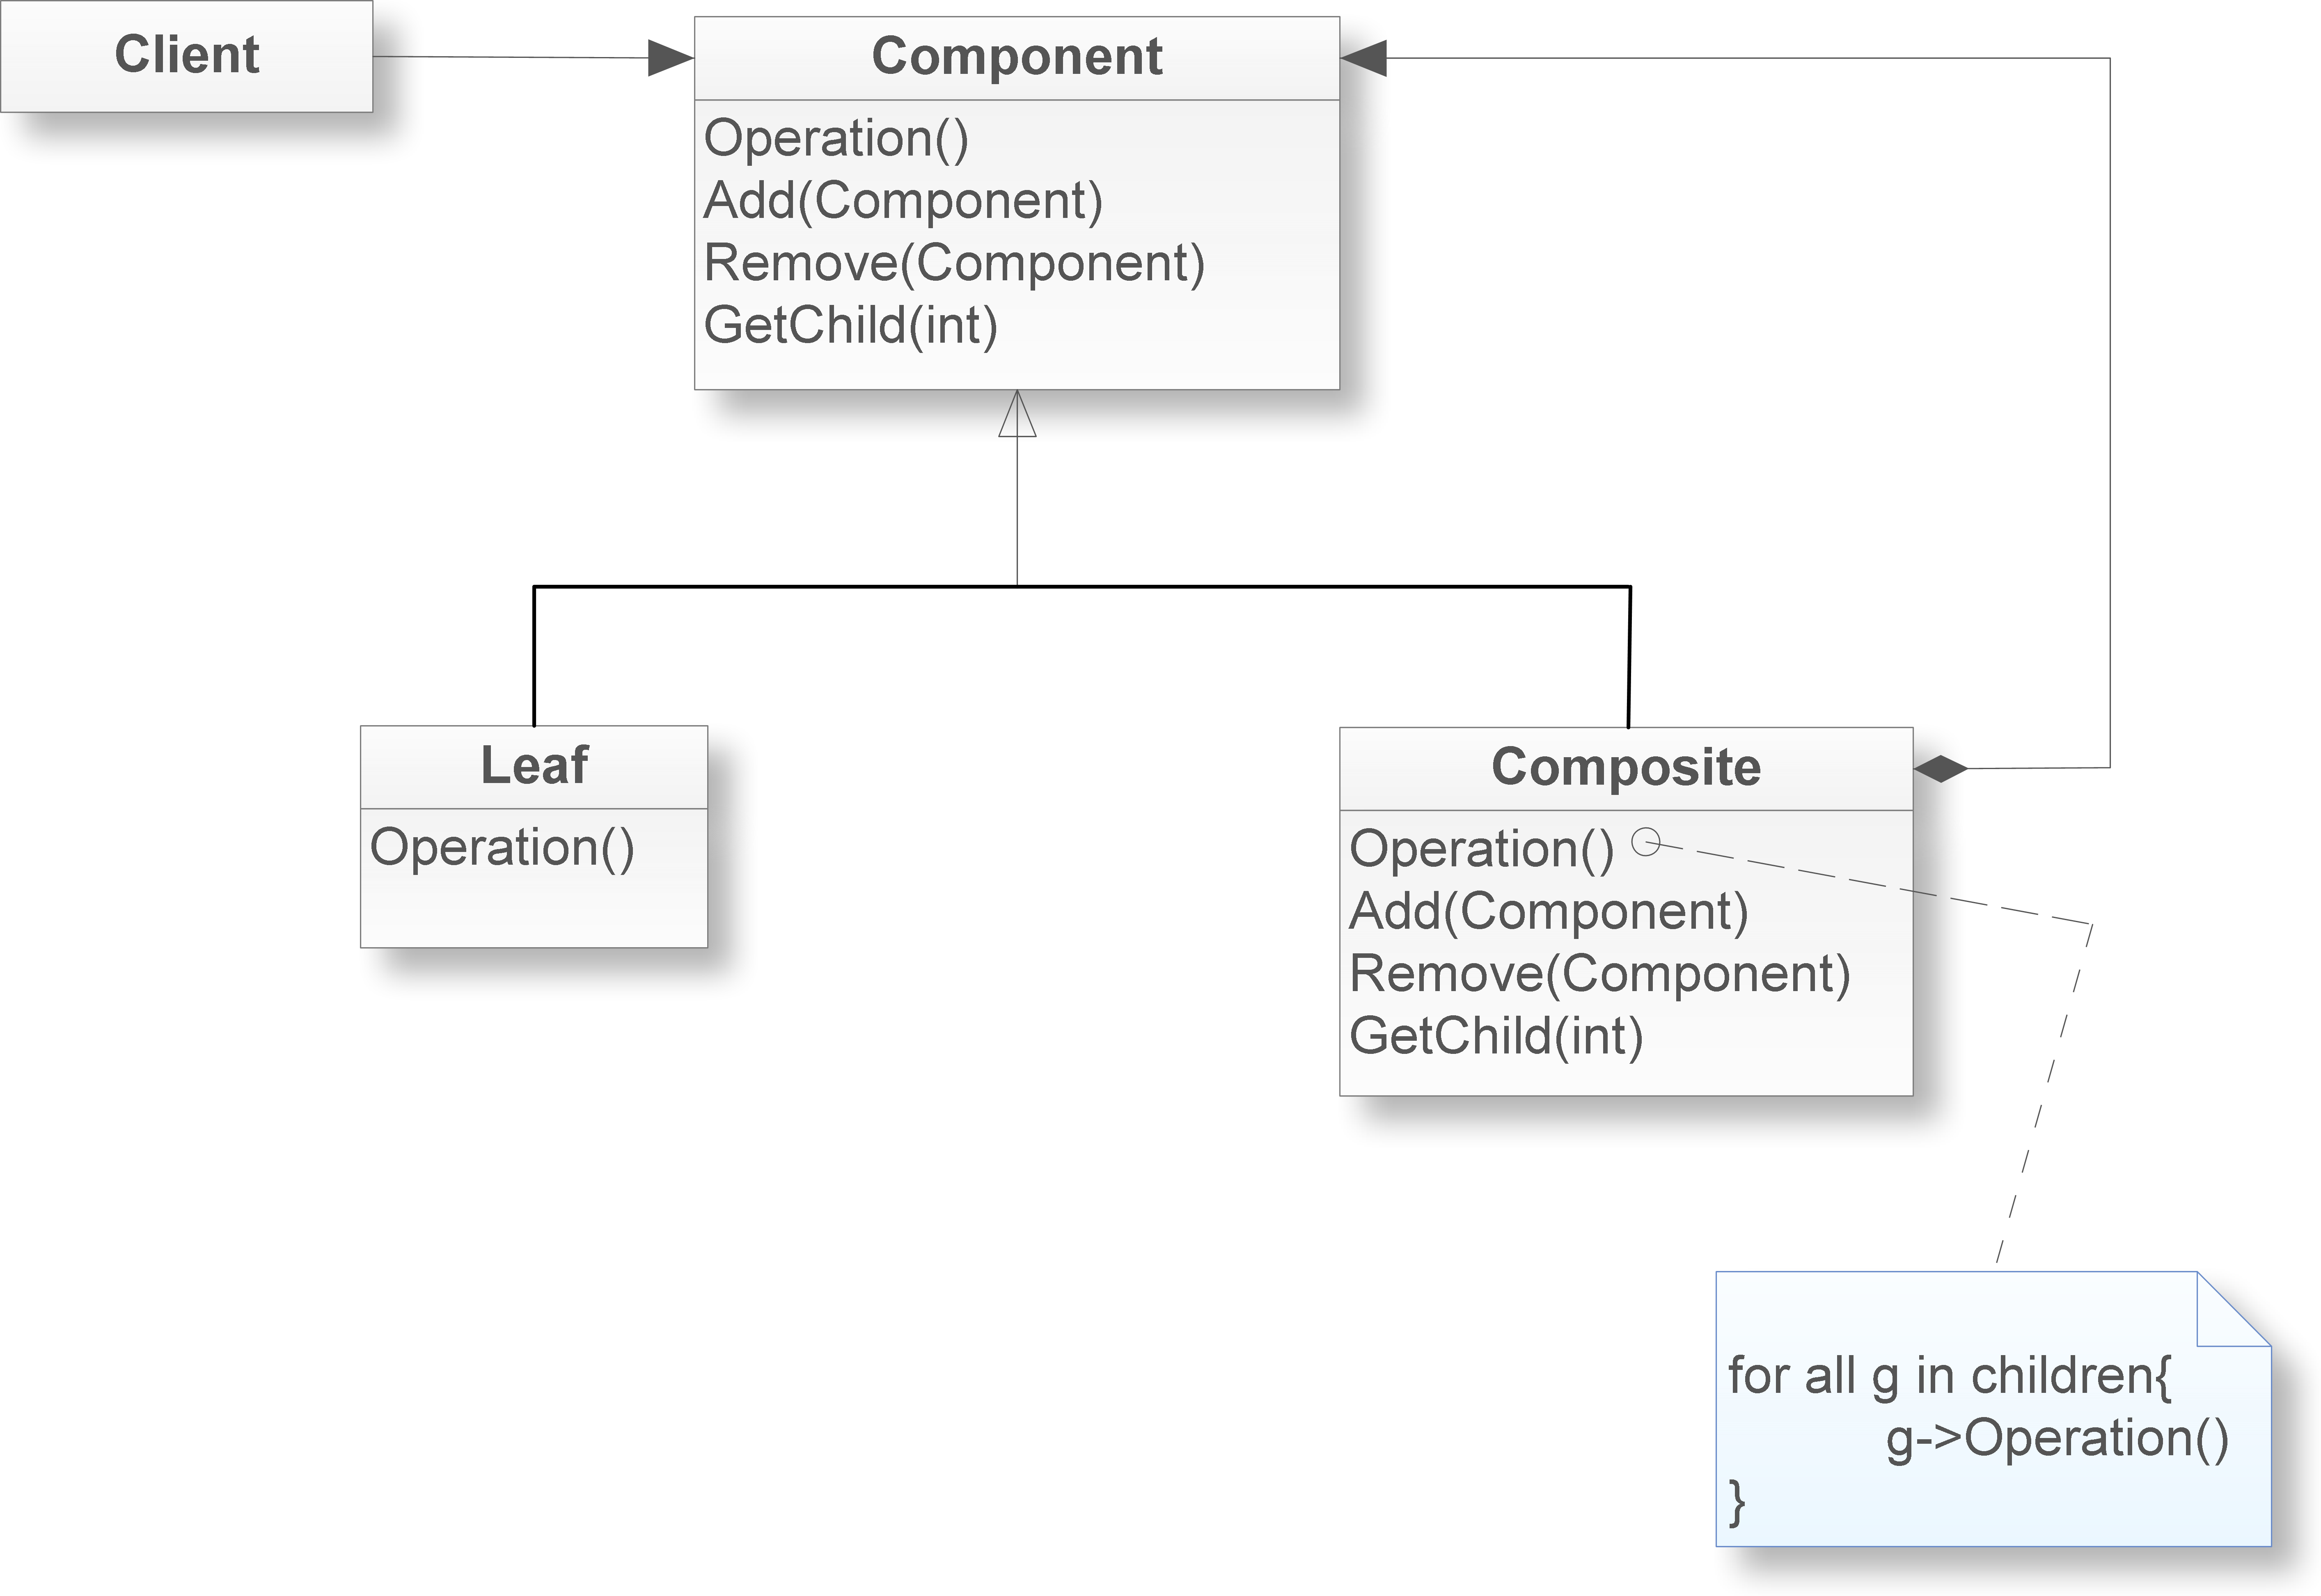
\includegraphics[width=.8\textwidth]{composite}
\caption{Diagramma ad alto livello del pattern Composite}\label{fig:composite}
\end{figure}

\subsubsection{Componenti che lo implementano}
\begin{description}
\item{\bfseries\scshape Gestione rubrica}\\
Composite permette di trattare in maniera omogenea singoli oggetti e oggetti composti, come gli utenti e gruppi di utenti della rubrica. Inoltre, dal momento che rende più semplice l'aggiunta di componenti, permetterebbe in futuro l'integrazione di nuove tipologie di utenti senza la necessità di modificare la struttura preesistente.

Lo svantaggio principale che comporta l'uso di Composite è la mancanza di limiti nell'aggiunta di nuove tipologie di componenti. Per far fronte a questo rischio si è introdotta la classe \texttt{org.softwaresynthesis.mytalk.server.abook.AddressBook} che controlla l'accesso alla struttura dati corrispondente alla rubrica.
\end{description}

\subsection{Data Access Object (DAO)}

\subsubsection{Scopo}
Il pattern DAO ha lo scopo di disaccoppiare la logica di business dalla logica di accesso ai dati. Questo si ottiene spostando la logica di accesso ai dati dai componenti di business ad una classe DAO rendendo i componenti che implementano la logica di business indipendenti dalla natura del dispositivo di persistenza. Questo approccio garantisce che un eventuale cambiamento del dispositivo di persistenza non comporti modifiche sui componenti di business.

\subsubsection{Diagramma esemplificativo}
\begin{figure}[H]
\centering
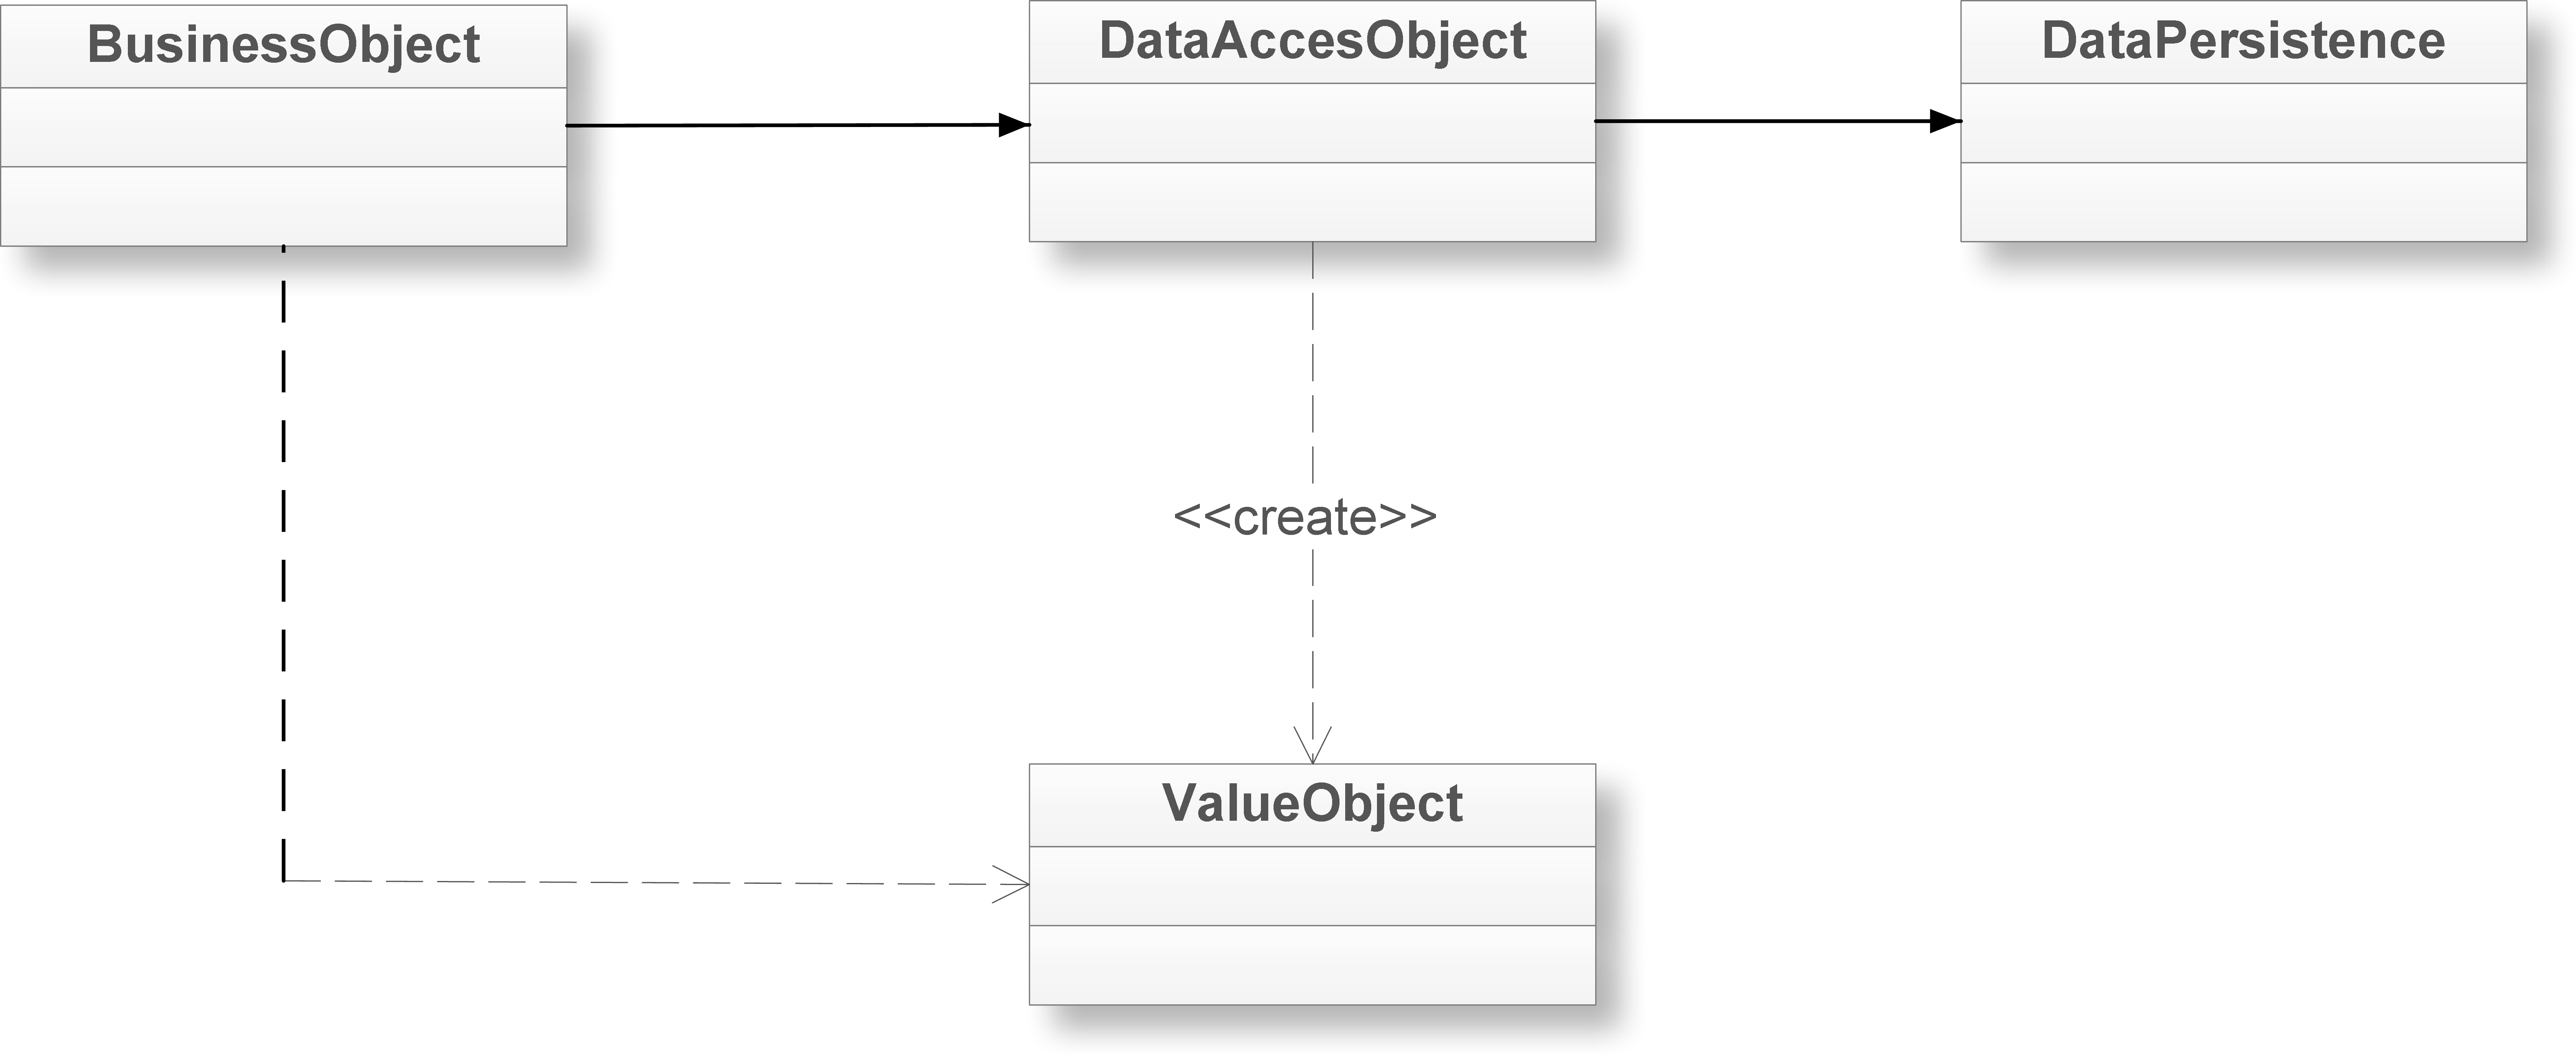
\includegraphics[width=.8\textwidth]{dao}
\caption{Diagramma ad alto livello del pattern Data Access Object}\label{fig:dao}
\end{figure}

\subsubsection{Componenti che lo implementano}
\begin{description}
\item{\scshape\bfseries Gestione Database}\\
Le classi DAO consentono di isolare l'accesso alle tabelle del \underline{database} dalla parte di business logic facendo corrispondere alle invocazioni di metodo le opportune operazioni sui record del \underline{database}.

L'utilizzo di tale pattern crea inoltre un maggiore livello di astrazione e mantiene una rigida separazione tra le sotto-architetture corrispondenti a model e presenter.
\end{description}

\subsection{Façade}

\subsubsection{Scopo}
Fornire un'interfaccia unificata per un insieme di interfacce o classi presenti in una sotto-architettura. Façade definisce inoltre un'interfaccia di livello più alto che rende la sotto-architettura più semplice da utilizzare.

\subsubsection{Diagramma esemplificativo}
\begin{figure}[H]
\centering
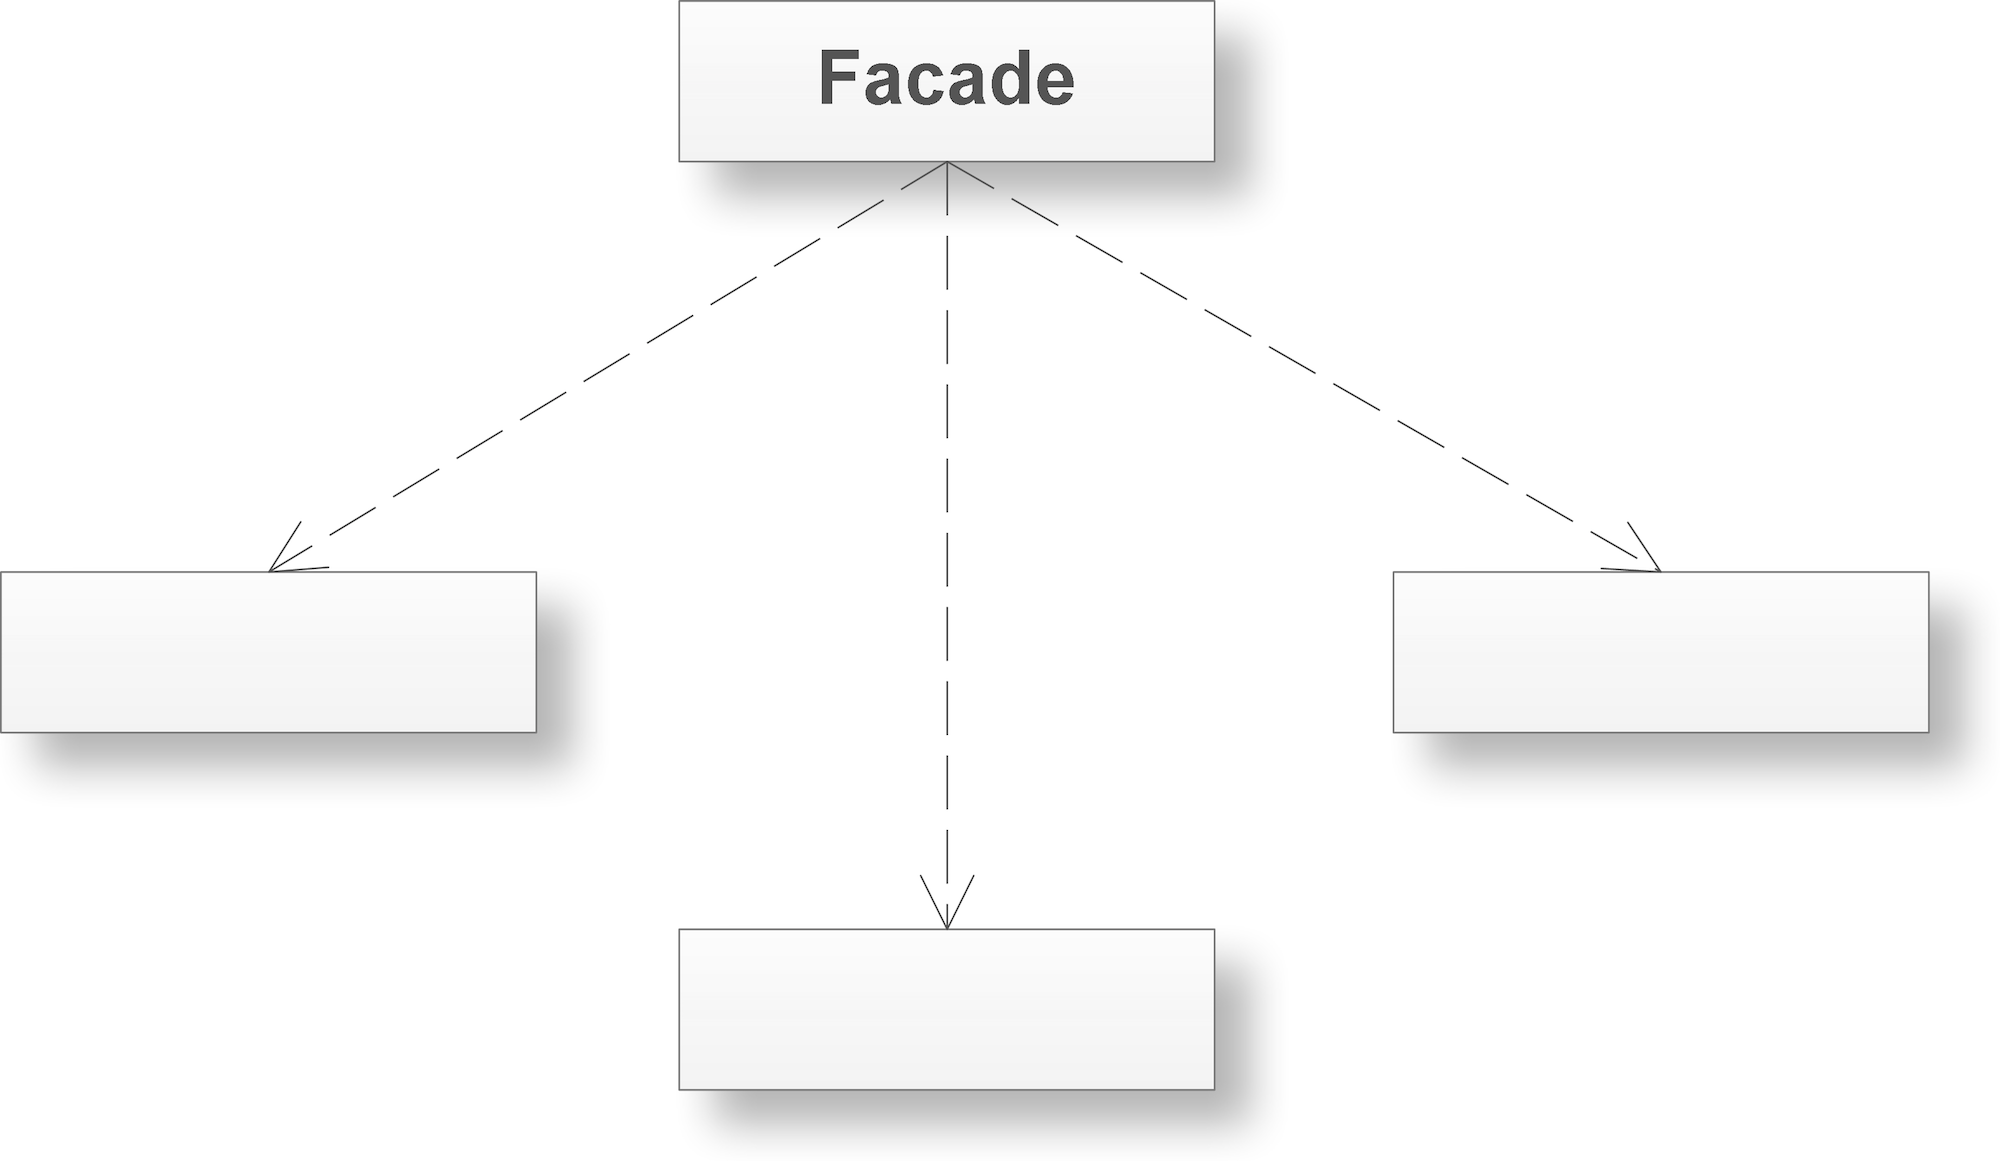
\includegraphics[width=.8\textwidth]{facade}
\caption{Diagramma ad alto livello del pattern Façade}\label{fig:façade}
\end{figure}

\subsubsection{Componenti che lo implementano}
\begin{description}
  \item{\scshape\bfseries Façade del server}\\
L'uso di Façade permette di esporre verso i \underline{client} una sorta di interfaccia semplificata nascondendo i componenti della sotto-architettura \underline{server}, fornendo un punto di accesso centralizzato e riducendo il numero di dipendenze funzionali fra le classi del \underline{server} e i componenti appartenenti a sotto-architetture esterne.
  \item{\scshape\bfseries Façade del presenter}\\
Tramite questo \underline{design pattern} si introduce un livello di indirettezza fra le sotto-architetture clientpresenter e clientview, che risultano dunque indipendenti.
  \item{\scshape\bfseries Façade della vista}\\
Data la forte bidirezionalità delle interazioni fra componenti delle sotto-architettura clientpresenter e clientview, è stata introdotta una sorta di facciata anche alla vista in modo da facilitare il tracciamento delle dipendenze fra i componenti del presenter e quelli della view.
\end{description}

\subsection{Factory Method}

\subsubsection{Scopo}
Definisce un'interfaccia per la creazione di un oggetto, lasciando alle sottoclassi la decisione sulla classe concreta che deve essere istanziata e consente di deferire l'istanziazione di una classe alle sottoclassi.

\subsubsection{Diagramma esemplificativo}
\begin{figure}[H]
\centering
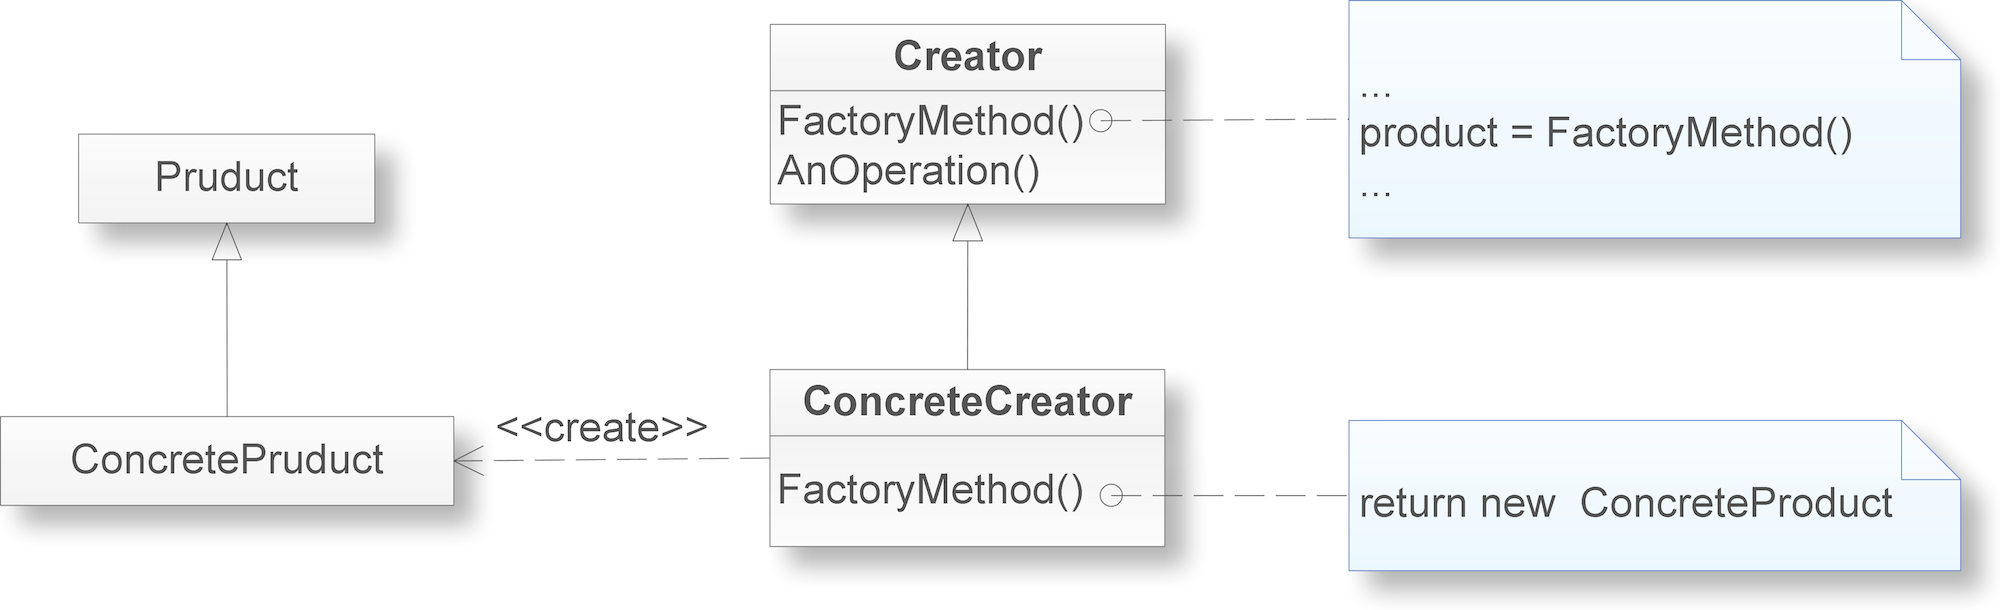
\includegraphics[width=.8\textwidth]{factory_method}
\caption{Diagramma ad alto livello del pattern Factory Method}\label{fig:factory_method}
\end{figure}

\subsubsection{Componenti che lo implementano}
\begin{description}
  \item{\scshape\bfseries Façade del server}\\
Factory Method permette ai \underline{client} di ottenere con facilità degli oggetti proxy che specializzano le interfacce \texttt{server.dao.IAudioMessage}, \texttt{server.dao.IAudioVideoMessage} e \texttt{server.dao.IUserData}.

Questo permette di ridurre il traffico di rete in quanto oggetti potenzialmente di grandi dimensioni rimangono sul \underline{server} e vengono scaricati solo quando se ne presenta l'effettiva necessità.
  \item{\scshape\bfseries Gestione connessione}\\
Gli oggetti che rappresentano connessioni, sottotipi di \texttt{server.connection.IConnection} sono ottenuti mediante un Factory Method nelle classi concrete che implementano l'interfaccia \texttt{server.connectionICommunicationHandler}.

Ciò garantisce maggiore flessibilità in quanto permette in futuro di gestire più categorie di handler che restituiscono diversi tipi connessione.
\end{description}

\subsection{Model-View-Presenter}

\subsubsection{Scopo}
Il pattern architetturale \foreignlanguage{english}{Model-View-Presenter} similmente a quanto accade per \foreignlanguage{english}{Model-View-Controller} (MVC), ha lo scopo di mantenere separata la \textit{business logic}, cioè la gestione dei dati secondo le regole di un determinato dominio e la loro memorizzazione in forma persistente, dalla presentazione e manipolazione mediante interfaccia utente.

\subsubsection{Diagrammi esemplificativi}
\begin{figure}[H]
\centering
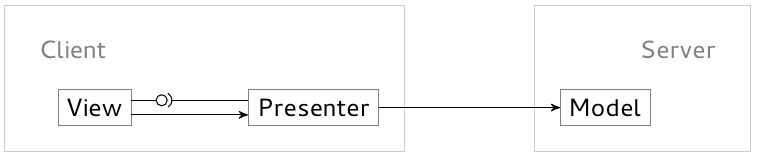
\includegraphics[width=.8\textwidth]{mvpHLdiagram}
\caption{Diagramma ad alto livello del pattern MVP}\label{fig:mvpHL}
\end{figure}

\begin{figure}[H]
\centering
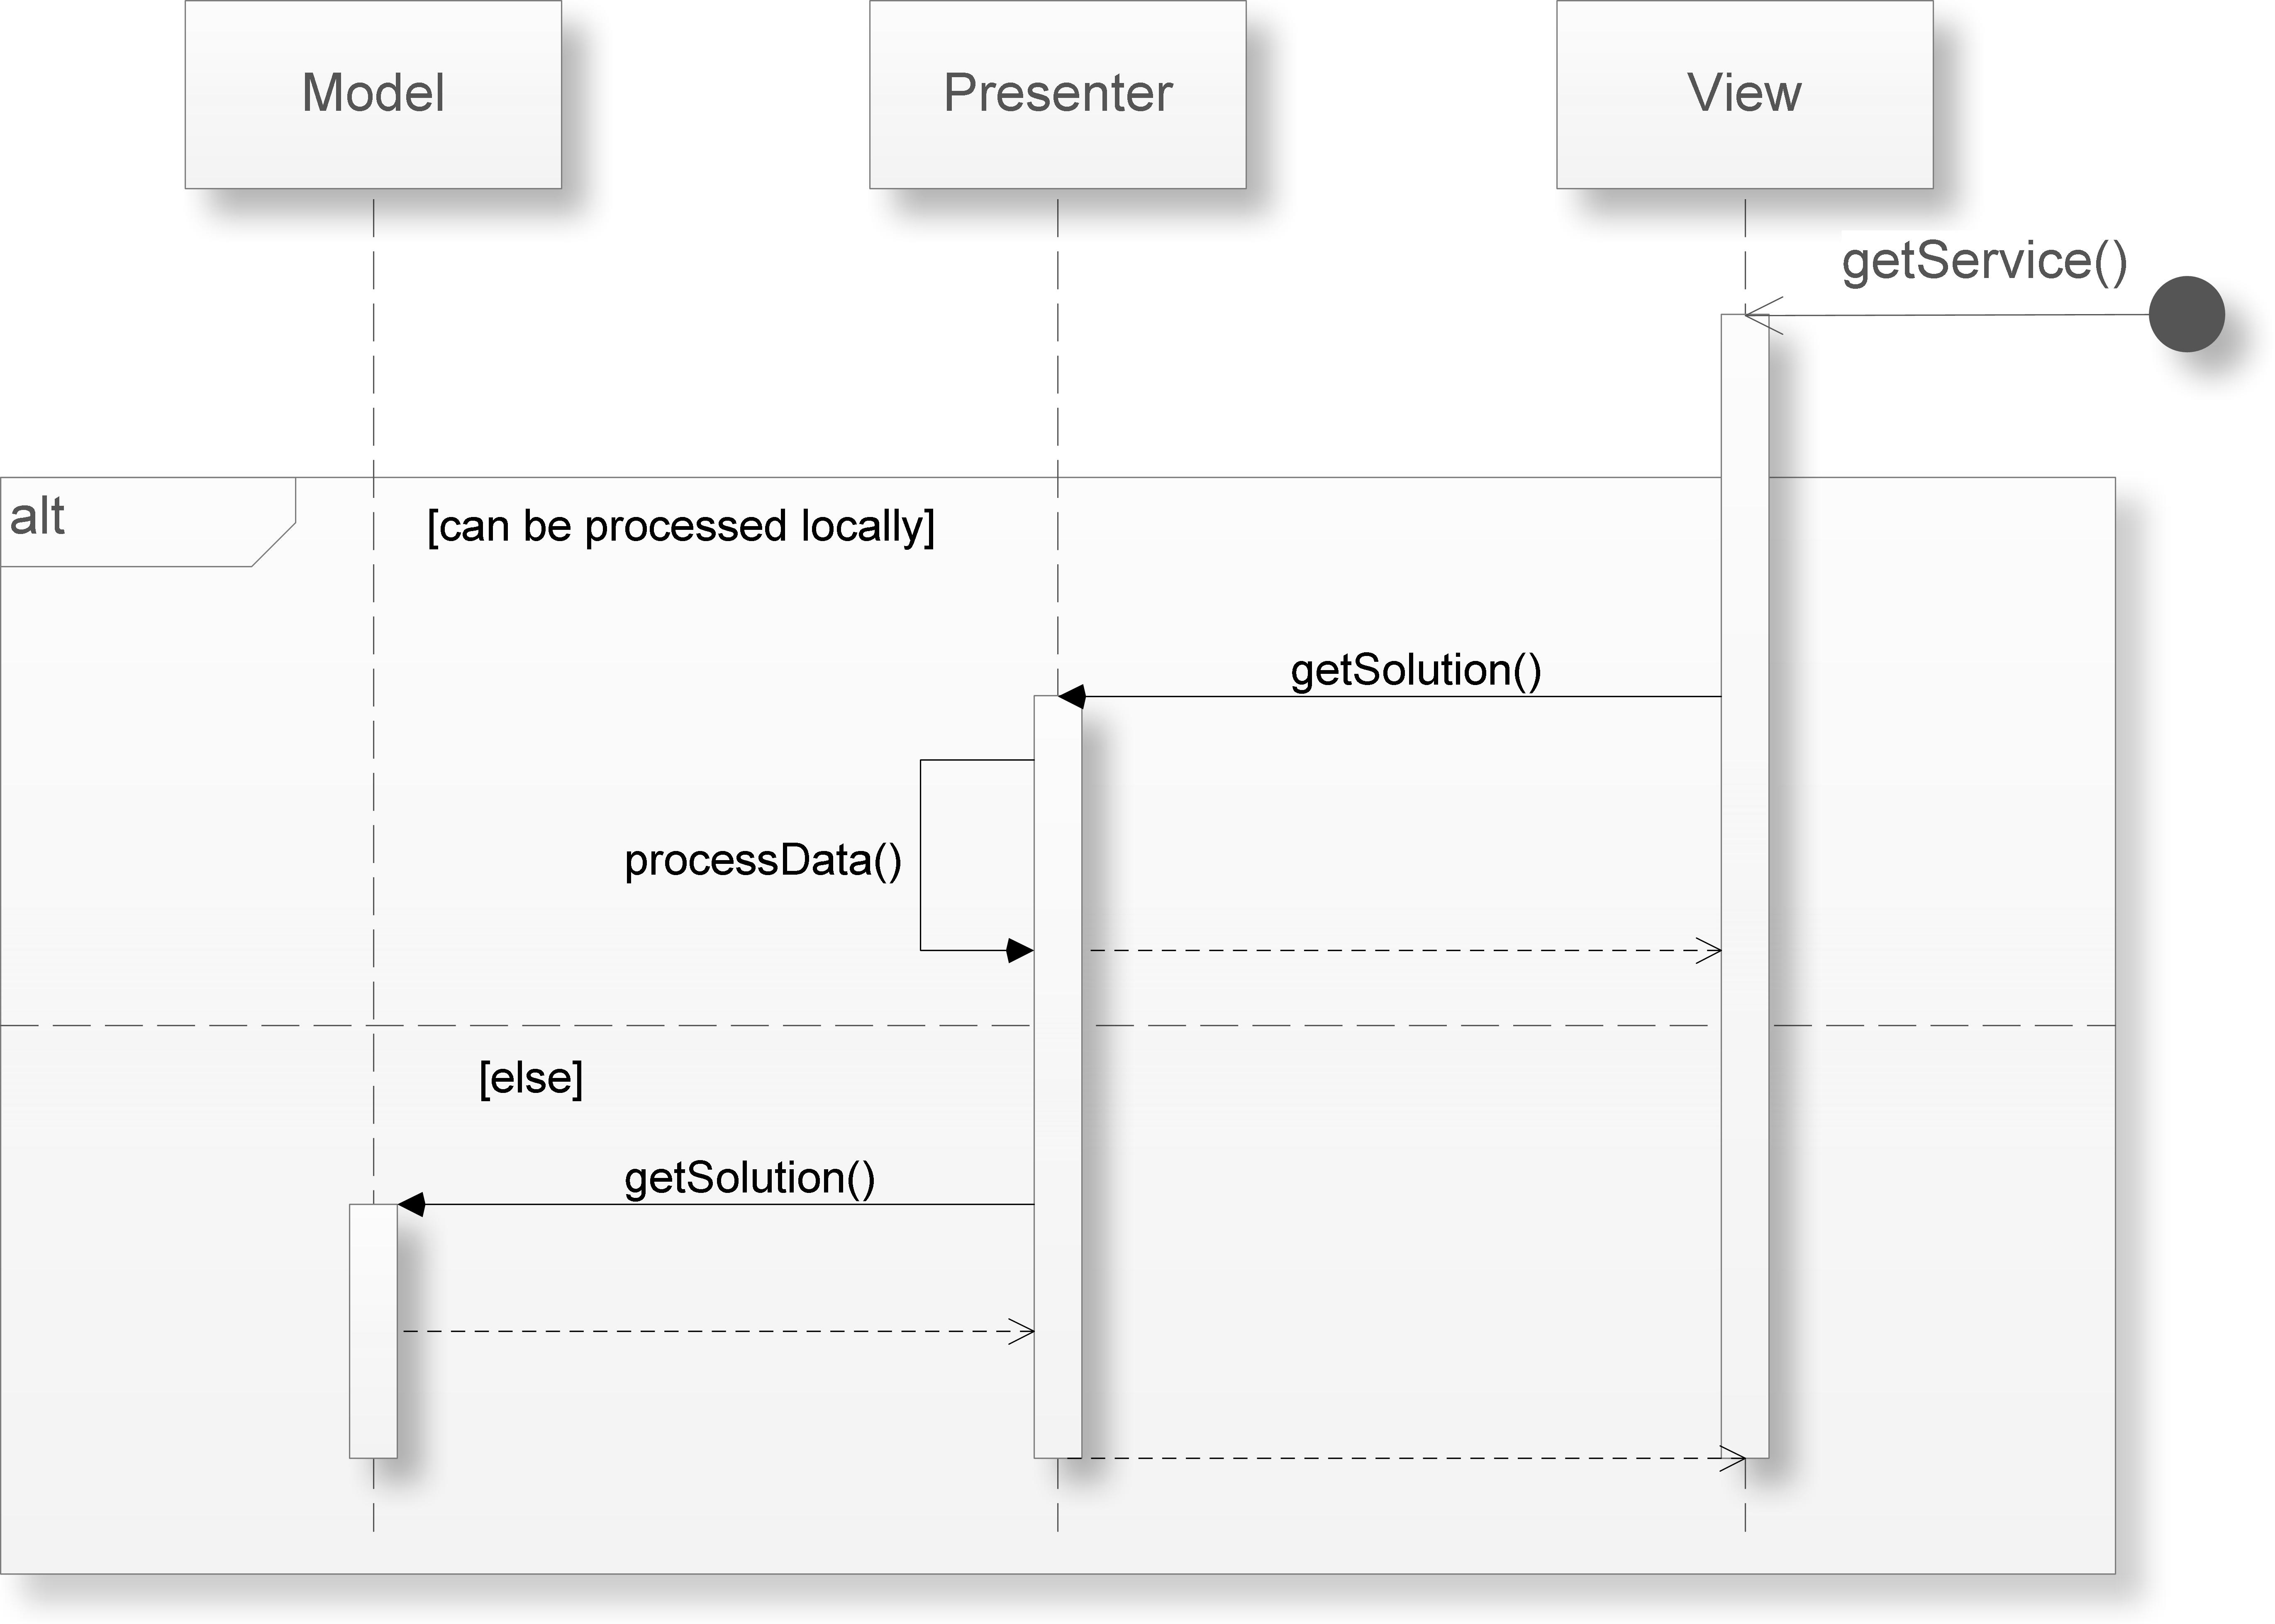
\includegraphics[width=\textwidth]{diagrammasequenzaMVP}
\caption{Diagramma di sequenza che illustra le collaborazioni in MVP}\label{fig:mvpSD}
\end{figure}

Come si evince dal diagramma riportato in figura \ref{fig:mvpSD} le interazioni avvengono solo tra view e presenter oppure tra presenter e model, senza che avvenga mai uno scambio di dati diretto fra model e view.

Ciò si deve al fatto che la business logic e il modello dei dati risiedono nel \underline{server} mentre il presenter e la view sono situati nel \underline{client}. Quando un utente richiede un servizio tramite l'interfaccia grafica, la richiesta viene inoltrata dalla view al presenter.

Qualora quest'ultimo fosse in grado di soddisfare tale richiesta con le risorse di cui dispone, i dati sono restituiti immediatamente alla view senza alcun bisogno di richiedere l'intervento del \underline{server}. Nel caso, invece, in cui il presenter non fosse in grado di servire autonomamente la view, interrogherebbe il \underline{server} al fine di ottenere i dati da restituire alla componente grafica.

Il vantaggio di un simile schema di interazione consiste nella riduzione del traffico di rete e nel conseguente incremento delle prestazioni in termini di velocità e, di conseguenza, dell'esperienza utente in generale.

\subsubsection{Componenti che lo implementano}
MVP viene utilizzato come il pattern più ad alto livello del nostro sistema. La distinzione fra model, presenter e view è infatti rispecchiata dalla suddivisione del sistema nelle tre sotto-architetture server, clientpresenter e clientview.

In generale, l'utilizzo di MVP riduce l'accoppiamento tra le sotto-architetture minimizzando le modifiche richieste a ognuno di essi come conseguenza di cambiamenti all'interno degli altri.

Inoltre, i componenti di questa sotto-architettura non sono vincolati a utilizzare la rete per accedere alle informazioni che sono memorizzate sul \underline{server} quando queste sono già disponibili (e possono essere elaborate) sul \underline{client}, migliorando quindi l'esperienza utente.

In particolare, le parti del sistema che usano questo pattern corrispondono alle sotto-architetture:
\begin{itemize}[noitemsep,nolistsep]
  \item server
  \item clientpresenter
  \item clientview
\end{itemize}

\subsection{Observer}

\subsubsection{Scopo}
Definire una dipendenza uno a molti fra oggetti, in modo tale che se un oggetto cambia il suo stato tutti gli oggetti dipendenti da questo siano notificati e aggiornati automaticamente.

\subsubsection{Diagramma esemplificativo}
\begin{figure}[H]
\centering
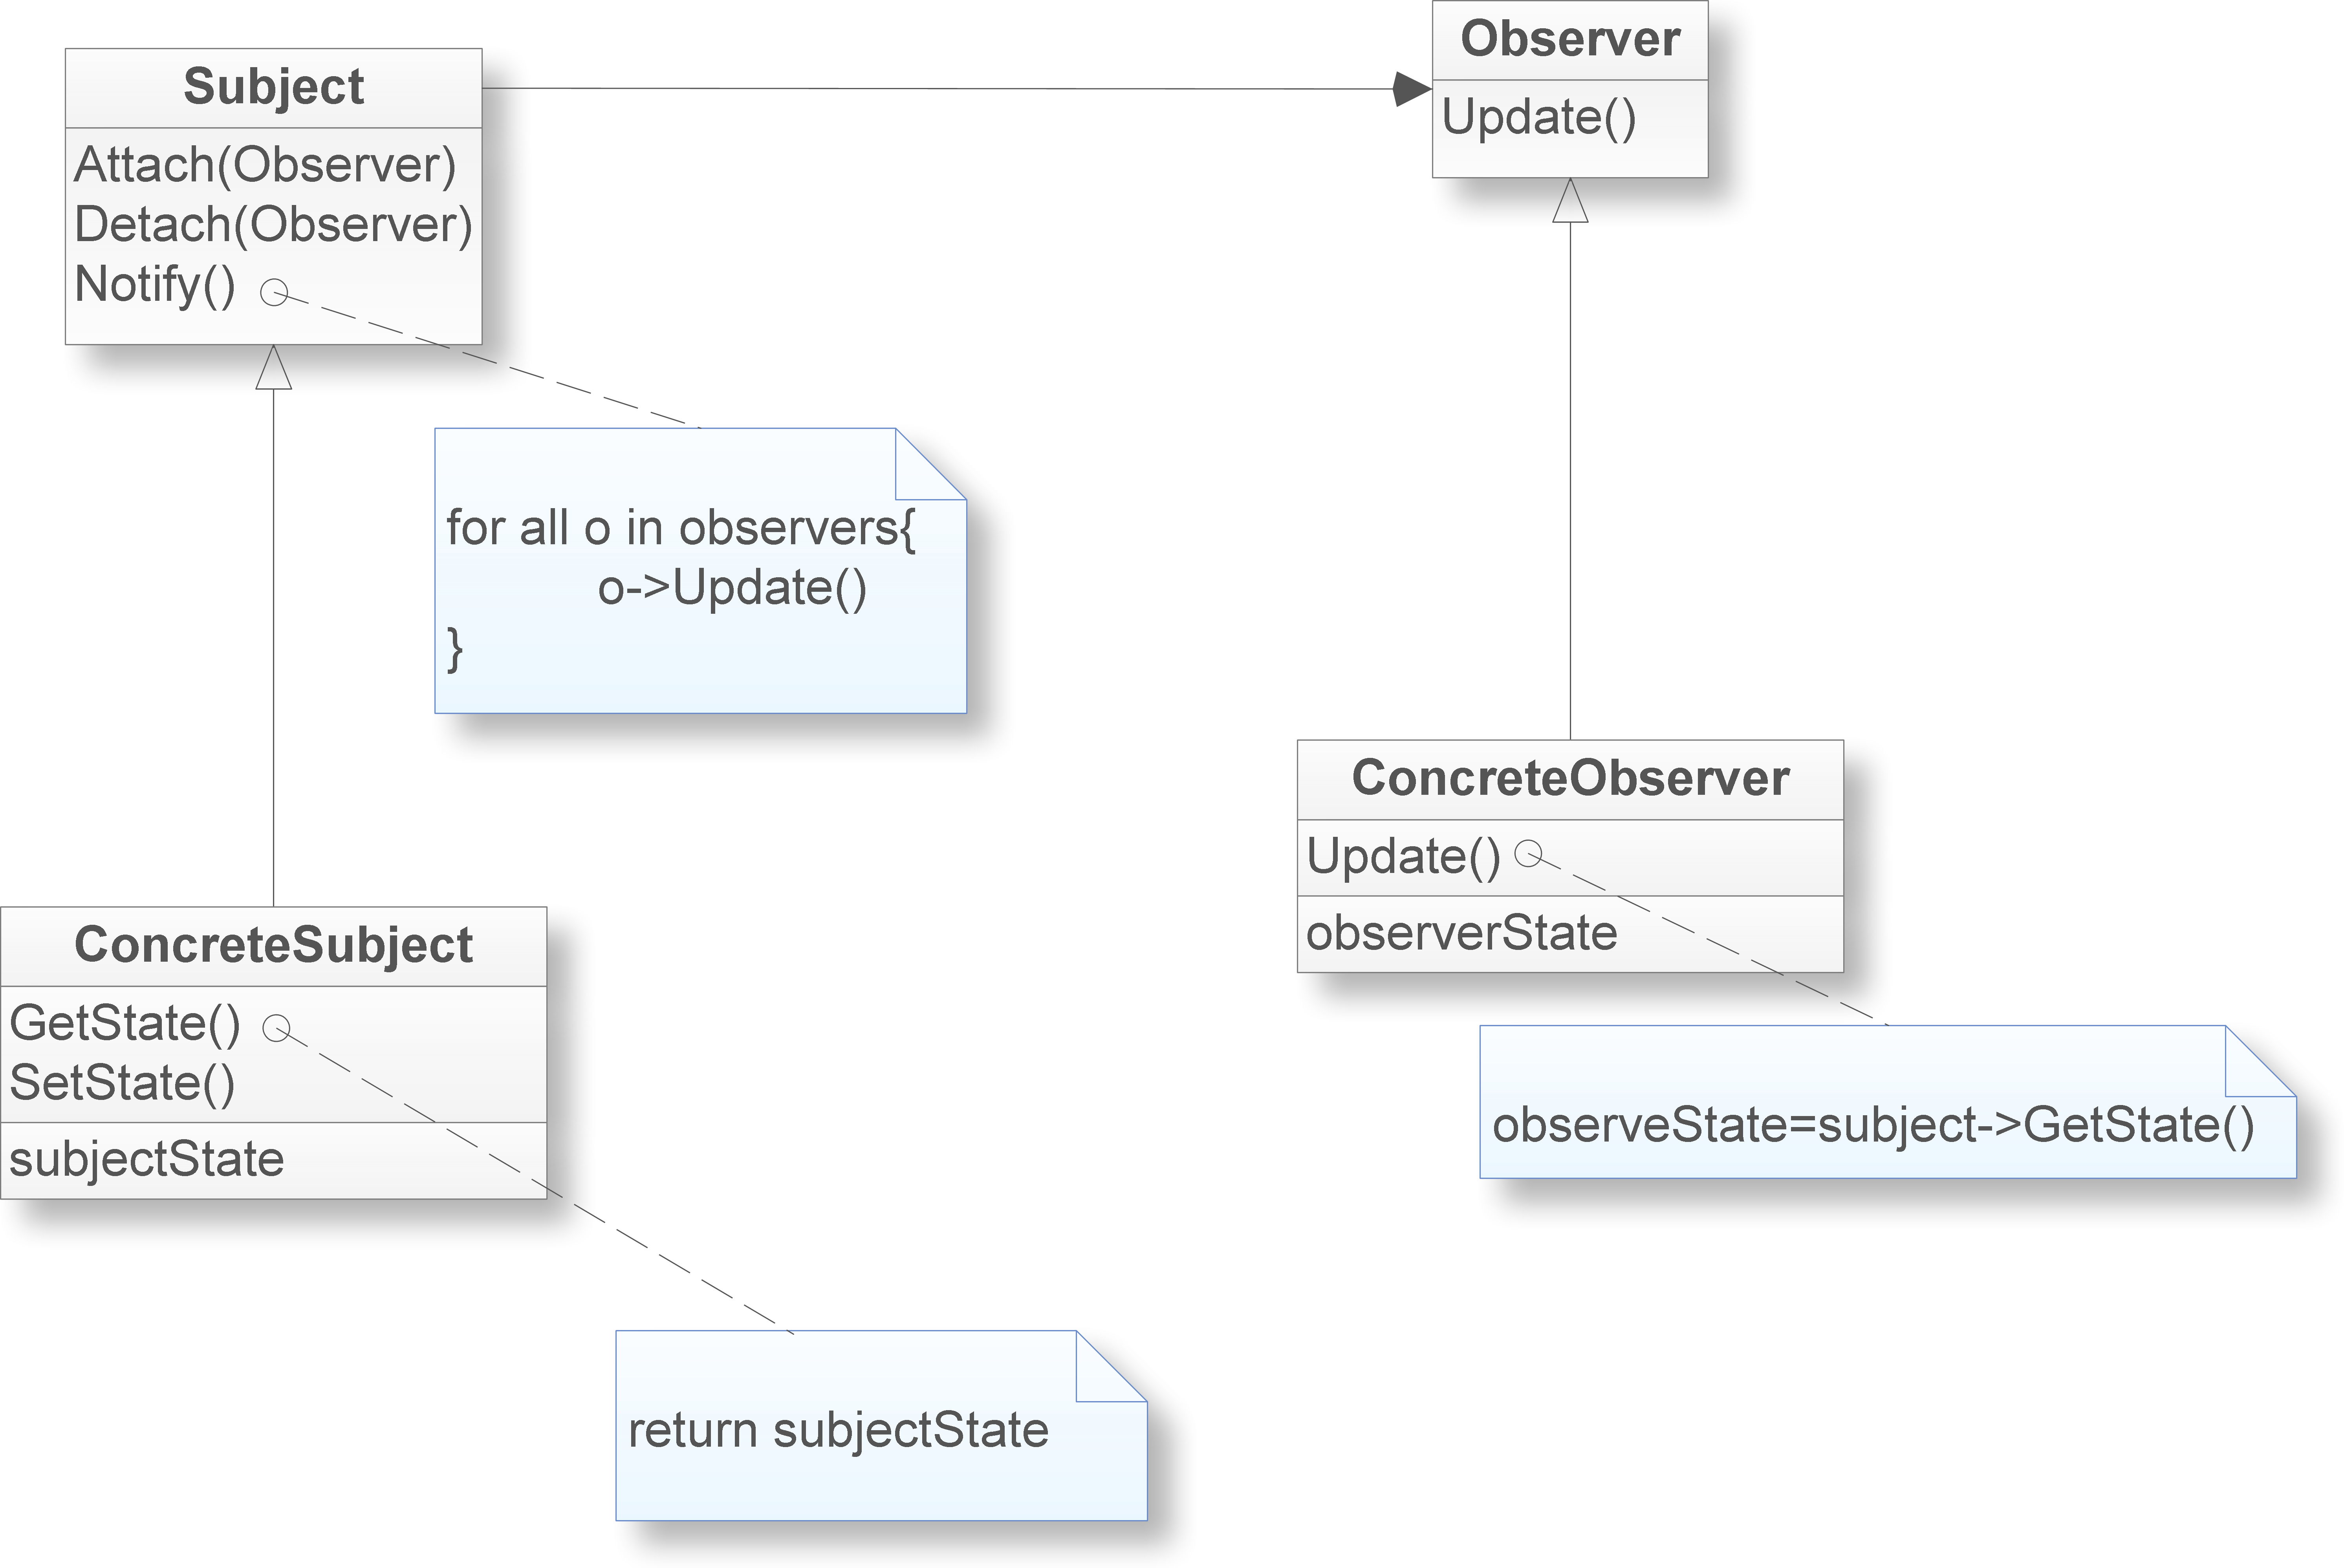
\includegraphics[width=.7\textwidth]{observer}
\caption{Diagramma ad alto livello del pattern Observer}\label{fig:observer}
\end{figure}

\subsubsection{Componenti che lo implementano}
\begin{description}
  \item{\scshape\bfseries Gestione stato}\\
Il pattern Observer è utile in quanto permette agli utenti di osservare lo stato degli altri, ricevendo in modo automatico e trasparente una notifica nel caso in cui uno di questi ultimi subisse variazioni, essendo ogni utente sia osservato che osservatore.

Al momento della connessione, infatti, ogni utente si registra come osservatore sui suoi contatti che sono online e, al contempo, li aggiunge tra i propri osservatori. In tal modo gli utenti notificano in broadcast le loro variazioni di stato e sono sempre aggiornati sullo stato dei contatti della loro rubrica.
\end{description}

\subsection{Proxy}

\subsubsection{Scopo}
Fornisce un placeholder per un altro oggetto in modo da controllarne l'accesso e consentire un uso ottimizzato della memoria.

\subsubsection{Diagramma esemplificativo}
\begin{figure}[H]
\centering
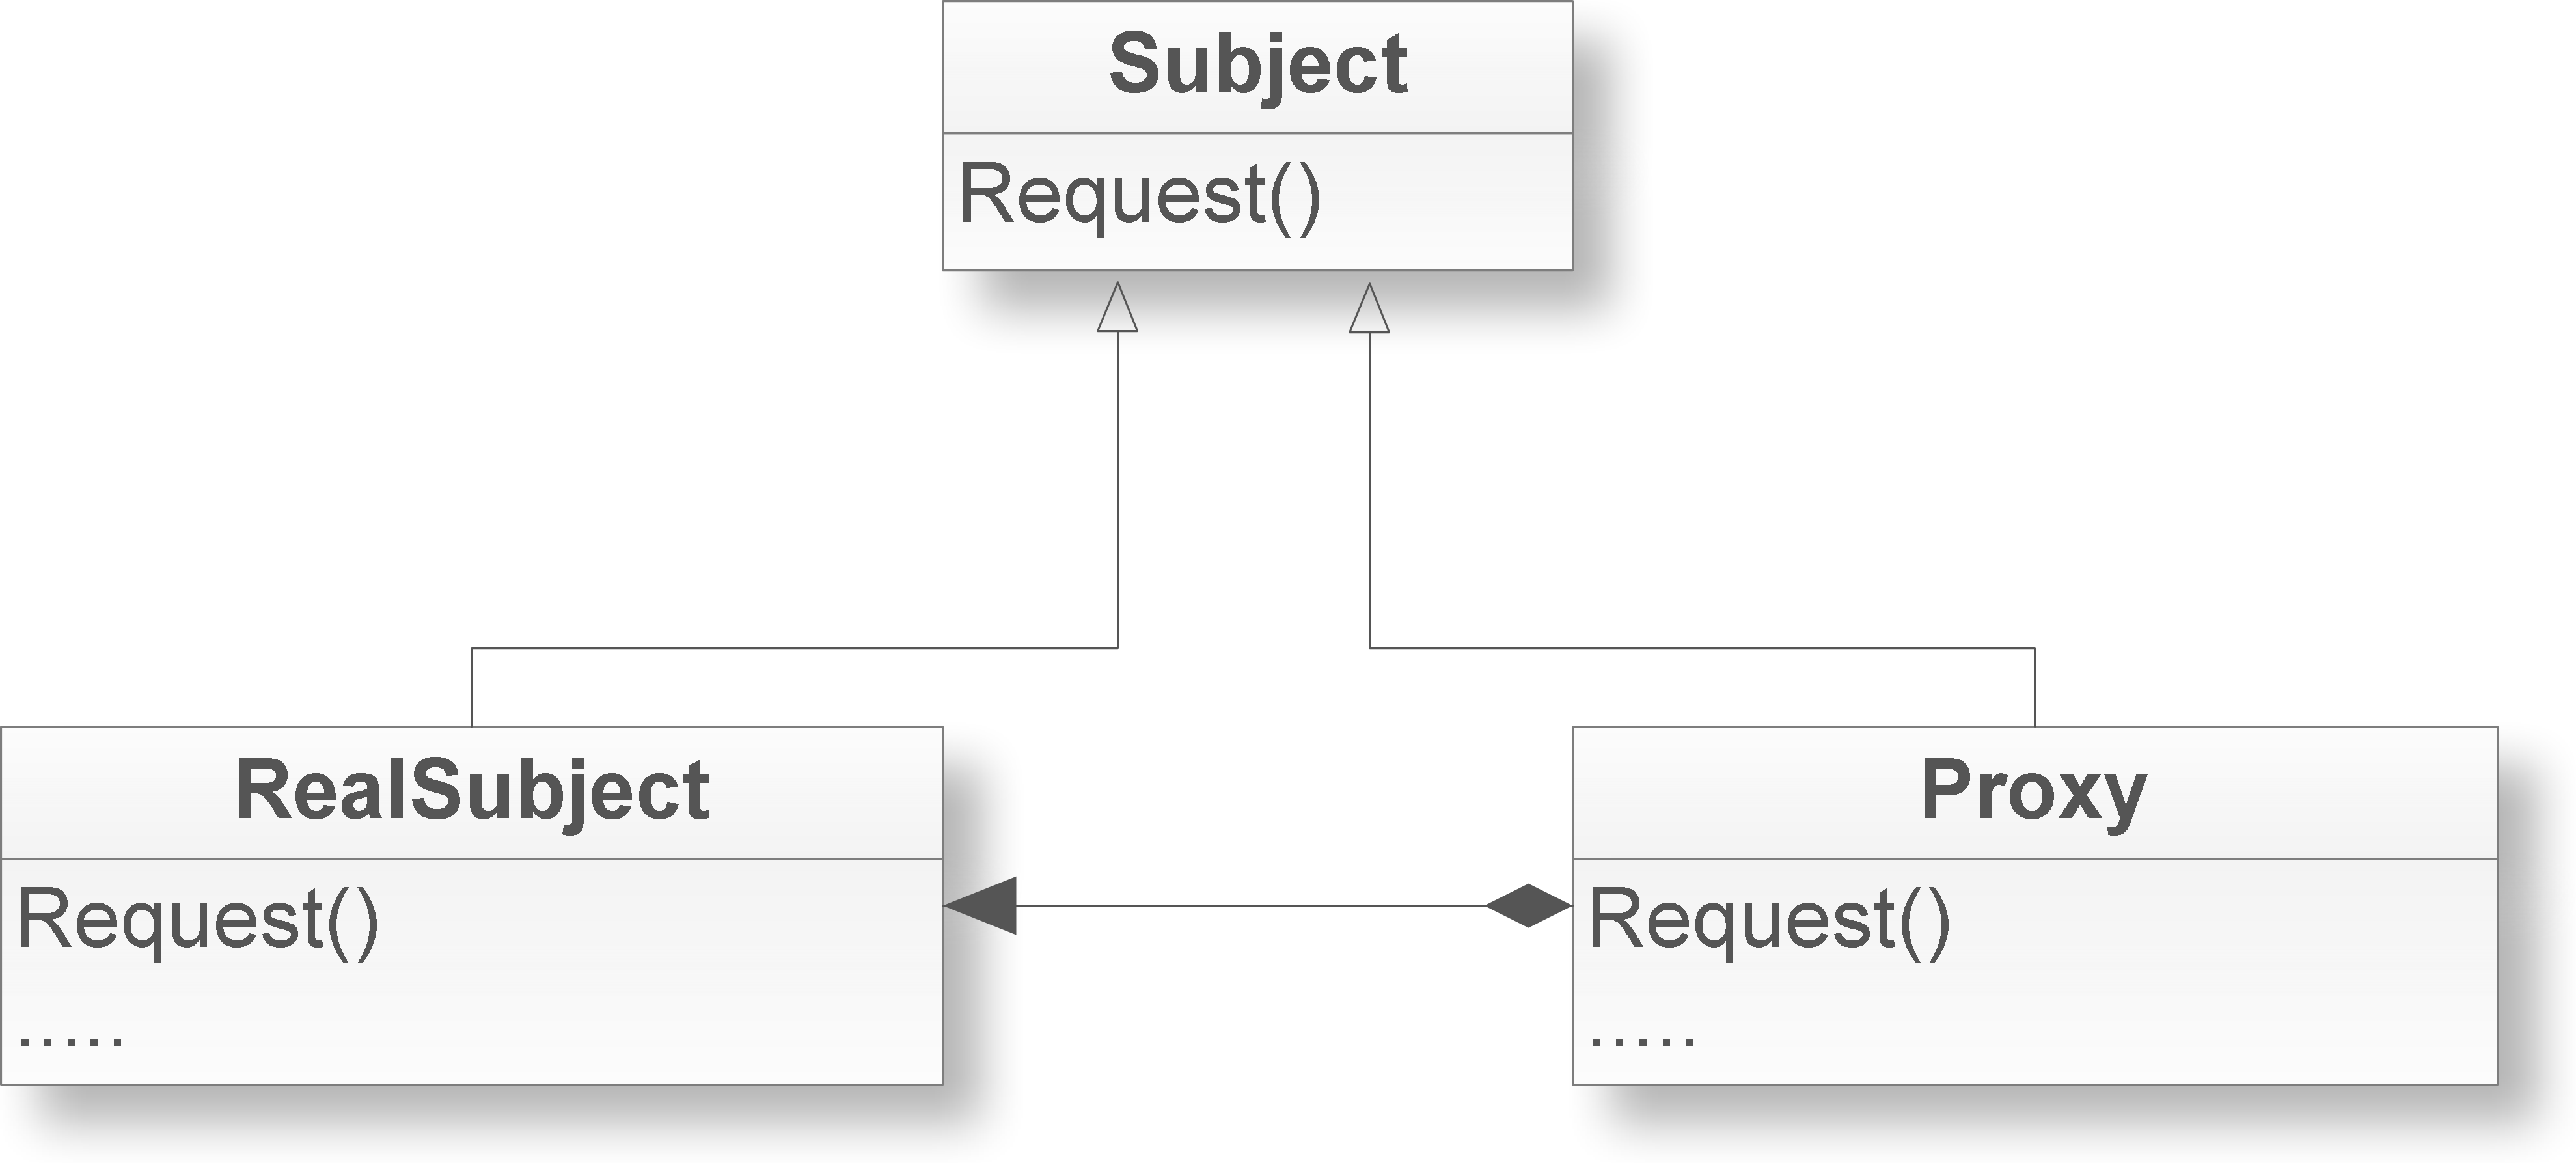
\includegraphics[width=.8\textwidth]{proxy}
\caption{Diagramma ad alto livello del pattern Proxy}\label{fig:proxy}
\end{figure}

\subsubsection{Componenti che lo implementano}
\begin{description}
  \item{\bfseries\scshape Gestione rubrica}\\
L'utilizzo di un proxy al posto di un utente permette di raggiungere una maggiore efficienza limitando l'utilizzo della rete evitando all'utente di percepire una eccessiva lentezza che comprometterebbe la sua esperienza.

Inoltre, tramite un proxy è possibile controllare l'accesso ai dati (che risiedono nel server) garantendo dunque un migliore livello di protezione.
  \item{\bfseries\scshape Gestione segreteria}\\
Poiché i messaggi audio e, soprattutto, i messaggi audio/video possono essere di grandi dimensioni, i proxy permettono di ottimizzare il consumo della memoria e di evitare l'attesa da parte dell'utente se non strettamente necessario.
\end{description}

\subsection{Singleton}

\subsubsection{Scopo}
Il pattern creazionale Singleton, garantisce che una determinata classe possa essere istanziata una sola volta, e di fornirne un punto di accesso globale. Questo pattern va utilizzato negli ambiti in cui si ha la necessità che l'accesso ad una determinata entità sia unico, in modo da permettere la gestione ottimale della risorsa stessa.

\subsubsection{Diagramma esemplificativo}
\begin{figure}[H]
\centering
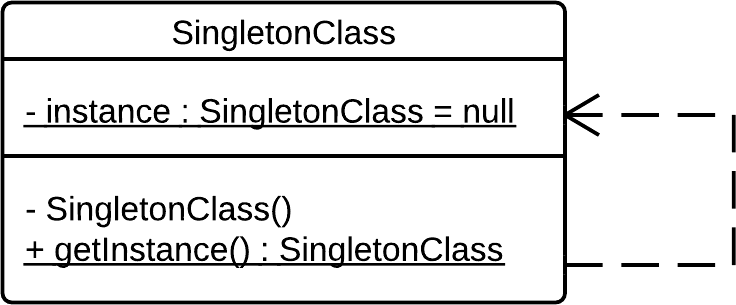
\includegraphics[width=.5\textwidth]{singleton}
\caption{Diagramma ad alto livello del pattern Singleton}\label{fig:singleton}
\end{figure}

\subsubsection{Componenti che lo implementano}
\begin{description}
  \item{\scshape\bfseries Façade del server}\\
Il pattern Singleton pone un limite superiore stretto al numero di istanze che possono esistere di una determinata classe e perciò è utile utilizzarlo per poter controllare il numero di oggetti \texttt{server.StandardServerFacade} che in questo caso è pari a uno. L'unicità dell'oggetto façade garantisce la presenza di un solo punto di accesso alle funzionalità dell sotto-architettura server.
  \item{\scshape\bfseries Façade del presenter}\\
Il pattern Singleton è altresì utile per controllare il numero di istanze attive della classe \texttt{clientpresenter.StandardPresenterFacade} per gli stessi motivi evidenziati in precedenza, ossia l'unicità del punto di accesso alle funzionalità della sotto-architettura clientpresenter.
  \item{\scshape\bfseries Gestione connessione}\\
La classe \texttt{server.connection.StandardConnectionHandler} è implementata come Singleton in modo da centralizzare la responsabilità di creare nuove connessioni in risposta alle esigenze dei \underline{client}.
  \item{\scshape\bfseries Façade della vista}\\
La classe \texttt{clientview.StandardViewFacade} è progettata in accordo con il \underline{design pattern} Singleton in modo da assicurare che in ogni momento ve ne sia una sola istanza attiva, responsabile di ricevere le richieste che giungono dal presenter.
  \item{\scshape\bfseries Gestione GUI}\\
Anche la classe \texttt{clientview.gui.GUIHandler} è implementata come Singleton in quanto permette di centralizzare la gestione delle collaborazioni fra le varie istanze attive delle classi grafiche.
\end{description}

\subsection{State}

\subsubsection{Scopo}
Permette ad un oggetto di cambiare il suo comportamento al variare del suo stato interno, quindi a run-time. L'oggetto si comporterà come se avesse cambiato la sua classe.

\subsubsection{Diagramma esemplificativo}
\begin{figure}[H]
\centering

\includegraphics[width=.7\textwidth]{state}
\caption{Diagramma ad alto livello del pattern State}\label{fig:state}
\end{figure}

\subsubsection{Componenti che lo implementano}
\begin{description}
\item{\scshape\bfseries Gestione dello Stato}\\
Il pattern State permette di gestire gli utenti del sistema determinando un comportamento diverso per questi ultimi a seconda del loro stato.

È stata definita un'apposita gerarchia di stati che permette quindi di specializzare nella maniera più adatta alle necessità del sistema le operazioni sugli utenti senza bisogno di condizionali annidati.
\end{description}
\clearpage

\section{Introduzione all'architettura di sistema}
Per introdurre l'architettura proposta è essenziale mettere in evidenza le seguenti considerazioni:
\begin{itemize}
	\item il sistema poggia su un \underline{database} nel quale sono contenuti i dati d'interesse per gli utenti (dati anagrafici, lista dei messaggi audio, lista dei messaggi audio e video, e la rubrica dei contatti);
	\item il sistema proposto dal team è dotato di una parte \underline{server} ed una parte \underline{client};
	\item dopo un'analisi preliminare il team ha stabilito che la progettazione del \underline{server} non deve essere vincolata da quella del \underline{client} in modo tale da evitare che il progetto dell'applicativo lato \underline{server} abbia la cognizione di come funziona il \underline{client}. Ciò permetterà un futuro riutilizzo del codice (e.g. se si desiderasse creare un nuovo applicativo di tipo \underline{VoIP} si potrà riutilizzare il \underline{server} già creato);
	\item per quanto riguarda il lato \underline{client}, al fine di garantire un alto livello di riutilizzo del codice e la possibilità di eseguire manutenzioni nel minor tempo possibile, si vuole che la logica d'implementazione del \underline{client} sia svincolata dalla rappresentazione grafica del medesimo.
\end{itemize}

Tali considerazioni di base, hanno portato il team a suddividere l'architettura in tre sotto-architetture, intese anche come package, più una quarta architettura inerente la struttura del \underline{database}:
\begin{itemize}
	\item il \underline{database};
	\item il \underline{server} (org.softwaresynthesis.mytalk.server);
	\item il clientpresenter (org.softwaresynthesis.mytalk.clientpresenter);
	\item il clientview (org.softwaresynthesis.mytalk.clientview).
\end{itemize}

Le specifiche di ogni sotto-architettura saranno definite in seguito, nelle relative sezioni.

Inoltre si fa presente che l'architettura generale, intesa come agglomerato delle tre sotto-architetture precedentemente elencate, fa uso del pattern MVP\@.

Sotto tale ottica la sotto-architettura \underline{server} ricopre il ruolo di model, il clientpresenter costituisce invece il presenter, mentre clientview è la vista definita per questo progetto. Tra le considerazioni più interessanti che hanno portato alla scelta di questo pattern, va messa in evidenza la seguente.

Assegnando ad ogni sotto-architettura un ruolo specifico, si garantisce un alto livello di riutilizzo del codice (e.g. clientview comunica con il presenter poiché non conosce la logica di business del sistema).

Quindi in un futuro di potrebbe riprendere la vista oggi definita, e riutilizzarla in un altro progetto, andando solo a ridefinire, se necessario, un presente che riproponga una nuovo adattamento della parte logica.

Di seguito verranno proposte le sotto-architetture evidenziate. Di ogni una sarà dato un elenco dettagliato dei componenti che lo interessano. Si sottolinea che per componenti non si intende i sottopackage, ma gli agglomerati di classi (potenzialmente prese da package diversi) che concorrono ad un fine comune: la definizione delle funzionalità del componente trattato.
\begin{figure}[H]
\begin{center}
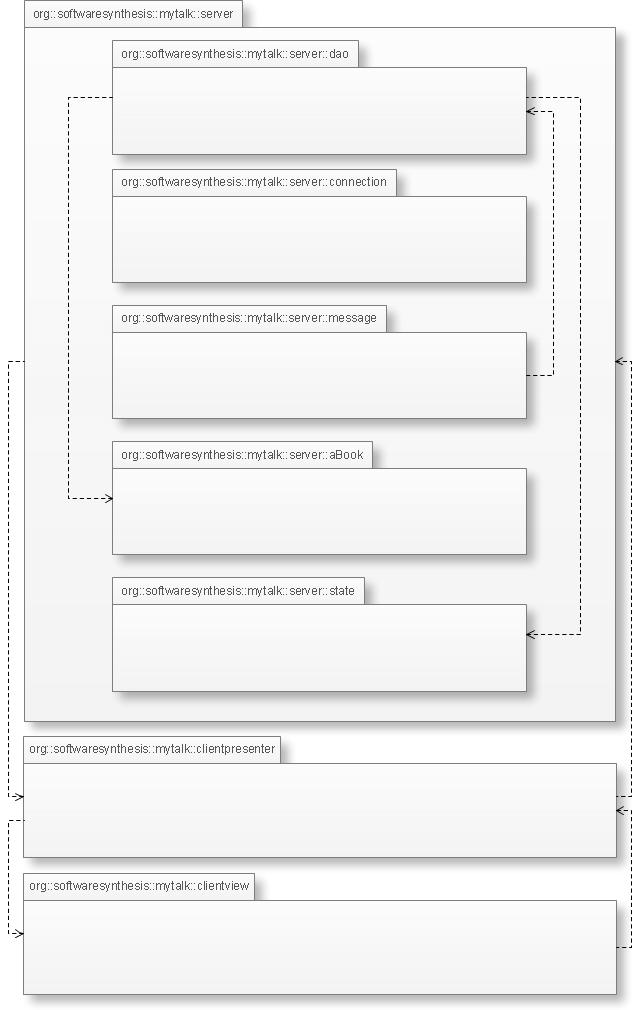
\includegraphics[width=.8\textwidth]{DiagrammaPackage}
\caption{Diagramma dei Package - Generale}\label{fig:package_generale}
\end{center}
\end{figure}


\clearpage

\section{Architettura del database}

Come già citato nella parte introduttiva all'architettura, il \underline{server} si appoggia ad un \underline{database} dove sono registrati i dati del sistema. La progettazione di tale \underline{database} passa per due fasi (come appreso dal manuale ``Sistemi di basi di dati''): la progettazione concettuale e la progettazione logica.

\subsection{Progettazione concettuale}
Con la progettazione concettuale definiremo una struttura ``concettuale'' della base di dati. Tale struttura non rappresenta quella finale pronta per la creazione su DBMS, ma bensì un modello in grado di rappresentare il problema, svincolato da come esso debba essere logicamente rappresentato.

\subsubsection{Lista delle classi}

\begin{description}
	\item{\scshape\bfseries UserData}: è l'entità le cui istanze rappresentano gli utenti registrati nel sistema. UserData è caratterizzata dai seguenti attributi:

\begin{center}
\rowcolors{2}{lightblue}{llightblue}
\begin{tabular}{lccc}
\toprule
Nome attributo & Tipo & Opzionale & Vincoli\\
\midrule % inserire qui il contenuto della tabella
E-Mail & Varchar(100) & NO & PrimaryKey\\
Password & Password & NO &\\
Question & Varchar(100) & NO &\\
Answer & Varchar(100) & NO &\\
Name & Varchar(100) & SI &\\
Cognome & Varchar(100) & SI &\\
Picture & Varchar(150) & SI &\\
\bottomrule
\end{tabular}
\end{center}

	\item{\scshape\bfseries Calls}: è l'entità le cui istanze rappresentano le chiamate effettuate attraverso il sistema software \caName. Calls è caratterizzata dai seguenti attributi:

\begin{center}
\rowcolors{2}{lightblue}{llightblue}
\begin{tabular}{lccc}
\toprule
Nome attributo & Tipo & Opzionale & Vincoli\\
\midrule % inserire qui il contenuto della tabella
ID & int & NO & PrimaryKey\\
Start\_date & Datetime & NO & \\
End\_date & Datetime & SI & \\
\bottomrule
\end{tabular}
\end{center}

	\item{\scshape\bfseries Groups}: è l'entità le cui istanze rappresentano un gruppo della rubrica di un utente. Tale entità è costituita dagli attributi:

\begin{center}
\rowcolors{2}{lightblue}{llightblue}
\begin{tabular}{lccc}
\toprule
Nome attributo & Tipo & Opzionale & Vincoli\\
\midrule % inserire qui il contenuto della tabella
Group\_ID & int & NO & PrimaryKey\\
Name & Varchar(100) & NO &\\
\bottomrule
\end{tabular}
\end{center}	
	
	\item{\scshape\bfseries Messages}: è l'entità che rappresenta le informazioni basilari di un messaggio della segreteria dell'utente. Gli attributi che la compongono sono:

\begin{center}
\rowcolors{2}{lightblue}{llightblue}
\begin{tabular}{lccc}
\toprule
Nome attributo & Tipo & Opzionale & Vincoli\\
\midrule % inserire qui il contenuto della tabella
Path & Varchar(150) & NO & PrimaryKey\\
Sender & Varchar(100) & NO & \\
Receiver & Varchar(100) & NO & \\
New & Boolean & NO & \\
\bottomrule
\end{tabular}
\end{center}	
	
	\item{\scshape\bfseries AudioMessages}: è un entità che specializza Messages e rappresenta i messaggi audio lasciati nella segreteria di un utente. L'entità non è caratterizzata da alcun attributo proprio.
	
	\item{\scshape\bfseries AudioVideoMessages}: è un entità che specializza Messages e rappresenta i messaggi audio/video lasciati nella segreteria di un utente.  L'entità non è caratterizzata da alcun attributo proprio.	
	
\end{description}

\subsubsection{Gerarchia tra classi}

\begin{description}
	\item{\scshape\bfseries Messages(AudioMessages e AudioVideoMessages)}: i messaggi si suddividono logicamente in due categorie, i messaggi dotati solamente di traccia audio e quelli aventi anche una traccia video. Gli attributi contenuti in queste entità sono gli stessi. Infatti la necessità di mostrare la separazione deriva dalla volontà del team di evidenziare la distinzione tra i due oggetti, motivata dalla possibilità di gestire le istanze delle due entità in modo diverso.
\end{description}

\subsubsection{Associazione tra classi}

\begin{description}
	\item{\scshape\bfseries UserData - Calls (molti a molti)}: tale associazione rappresenta il legame che intercorre tra gli utenti e le chiamate. Tale associazione è del tipo molti a molti, con totalità parziale verso Calls e totalità totale verso UserData.
	\item{\scshape\bfseries UserData - Groups (molti a molti)}: tale associazione rappresenta il legame che intercorre tra gli utenti ed i gruppi, per la quale si è deciso di usare un associazione molti a molti con totalità parziale solo da Groups a UserData. Ciò significa che: un utente può comparire in zero o più gruppi (in ragione del fatto che potrebbe esserci più di qualcuno che registra un dato utente nella propria rubrica), ed un utente può possedere uno o più gruppi.
	\item{\scshape\bfseries UserData - Groups (uno a molti)}: tale associazione rappresenta il legame che intercorre tra il proprietario del gruppo e il gruppo stesso. L'associazione è del tipo uno a molti, a rappresentare come un gruppo sia visualizzabile unicamente dal proprietario, mentre un utente può avere (e di conseguenza visualizzare) più gruppi.
	\item{\scshape\bfseries UserData - Messages (uno a molti)}: tale associazione rappresenta il legame che intercorre tra gli utenti ed i messaggi registrati nella sua segreteria. L'associazione è del tipo uno a molti verso Messages, con totalità parziale verso Messages e totalità totale verso UserData. L'idea alla base è che un utente può avere nella propria segreteria uno o più messaggi, così come può non averne nessuno, mentre ogni messaggio della segreteria è ``visionabile'' da un unico utente, il destinatario del messaggio.
\end{description}

\subsection{Progettazione logica}
Con la progettazione logica intendiamo costruire la struttura definitiva del \underline{database} sulla base della progettazione concettuale. Quindi si deciderà come trasformare le gerarchie e in seguito le associazioni, al fine di restituire una struttura chiara e pronta per la creazione sul DBMS\@. La lista delle classi proposta, e lo schema associato, rappresentano tale struttura.

\subsubsection{Rappresentazione delle gerarchie}

\begin{description}
	\item{\scshape\bfseries Messages(AudioMessages e AudioVideoMessages)}: al fine di evidenziare la suddivisione logica tra le due tipologie di messaggi, è stato deciso di trasformare la specializzazione di Messages con una tabella unica contenente un discriminante. È rimasta esclusivamente l'entità Messages a cui è stato aggiunto l'attributo ``Audio'' con la funzione di discriminare le due tipologie di messaggi.
\end{description}

\subsubsection{Rappresentazione delle associazioni}

\begin{description}
	\item{\scshape\bfseries UserData - Calls}: tale associazione si è risolta attraverso l'introduzione dell'entità CallLists. Tale entità contiene l'attributo User come chiave esterna verso l'entità UserData e l'attributo Call\_ID come chiave esterna verso l'entità Calls. È dotata inoltre dell'attributo Caller che identifica colui che ha per primo avviato la chiamata; per ogni gruppo di ennuple aventi lo stesso Call\_ID si avrà soltanto una ennupla contrassegnata con il campo Caller a vero.
	\item{\scshape\bfseries UserData - Groups}: tale associazione si è risolta con la creazione di una terza entità denominata AddressBooks, che contiene una chiave esterna verso UserData e una chiave esterna verso Groups.
	\item{\scshape\bfseries UserData - Groups}: tale associazione si è risolta trasformando l'attributo Owner in una chiave esterna verso UserData.
	\item{\scshape\bfseries UserData - Messages}: tale associazione si è risolta inserendo una chiave esterna verso UserData, all'interno dell'entità Messages.
\end{description}

\subsubsection{Lista delle classi}

\begin{center}

UserData

\rowcolors{2}{lightblue}{llightblue}
\begin{center}
\begin{tabular}{lccc}
\toprule
Nome attributo & Tipo & Opzionale & Vincoli\\
\midrule % inserire qui il contenuto della tabella
E-Mail & Varchar(100) & NO & PrimaryKey\\
Password & Password & NO &\\
Question & Varchar(100) & NO &\\
Answer & Varchar(100) & NO &\\
Name & Varchar(100) & SI &\\
Surname & Varchar(100) & SI &\\
Picture & Varchar(150) & SI &\\
\bottomrule
\end{tabular}
\end{center}

Calls

\begin{center}
\rowcolors{2}{lightblue}{llightblue}
\begin{tabular}{lccc}
\toprule
Nome attributo & Tipo & Opzionale & Vincoli\\
\midrule % inserire qui il contenuto della tabella
ID & int & NO & PrimaryKey\\
Start\_date & Datetime & NO & \\
End\_date & Datetime & SI &\\
\bottomrule
\end{tabular}
\end{center}

CallLists

\begin{center}
\rowcolors{2}{lightblue}{llightblue}
\begin{tabular}{lccc}
\toprule
Nome attributo & Tipo & Opzionale & Vincoli\\
\midrule % inserire qui il contenuto della tabella
Call\_ID & int & NO & PrimaryKey e ForeignKey verso Calls\\
User & Varchar(100) & NO & PrimaryKey e ForeignKey verso UserData \\
Caller & Boolean & NO &\\
\bottomrule
\end{tabular}
\end{center}

AddressBooks

\begin{center}
\rowcolors{2}{lightblue}{llightblue}
\begin{tabular}{lccc}
\toprule
Nome attributo & Tipo & Opzionale & Vincoli\\
\midrule % inserire qui il contenuto della tabella
User\_ID & Varchar(100) & NO & PrimaryKey e ForeignKey verso UserData\\
Group\_ID & int & NO & PrimaryKey e ForeignKey verso Groups\\
\bottomrule
\end{tabular}
\end{center}

Groups

\begin{center}
\rowcolors{2}{lightblue}{llightblue}
\begin{tabular}{lccc}
\toprule
Nome attributo & Tipo & Opzionale & Vincoli\\
\midrule % inserire qui il contenuto della tabella
Group\_ID & int & NO & PrimaryKey\\
Name & Varchar(100) & NO & \\
Owner & Varchar(100) & NO & ForeignKey verso UserData\\
\bottomrule
\end{tabular}
\end{center}	

Messages

\begin{center}
\rowcolors{2}{lightblue}{llightblue}
\begin{tabular}{lccc}
\toprule
Nome attributo & Tipo & Opzionale & Vincoli\\
\midrule % inserire qui il contenuto della tabella
Path & Varchar(150) & NO & PrimaryKey\\
Sender & Varchar(100) & NO & ForeignKey verso UserData \\
Receiver & Varchar(100) & NO & ForeignKey verso UserData\\
New & Boolean & NO & \\
Audio & Boolean & NO & \\
\bottomrule
\end{tabular}	
\end{center}

\end{center}

\subsubsection{Diagramma delle classi}
\begin{figure}[H]
\begin{center}
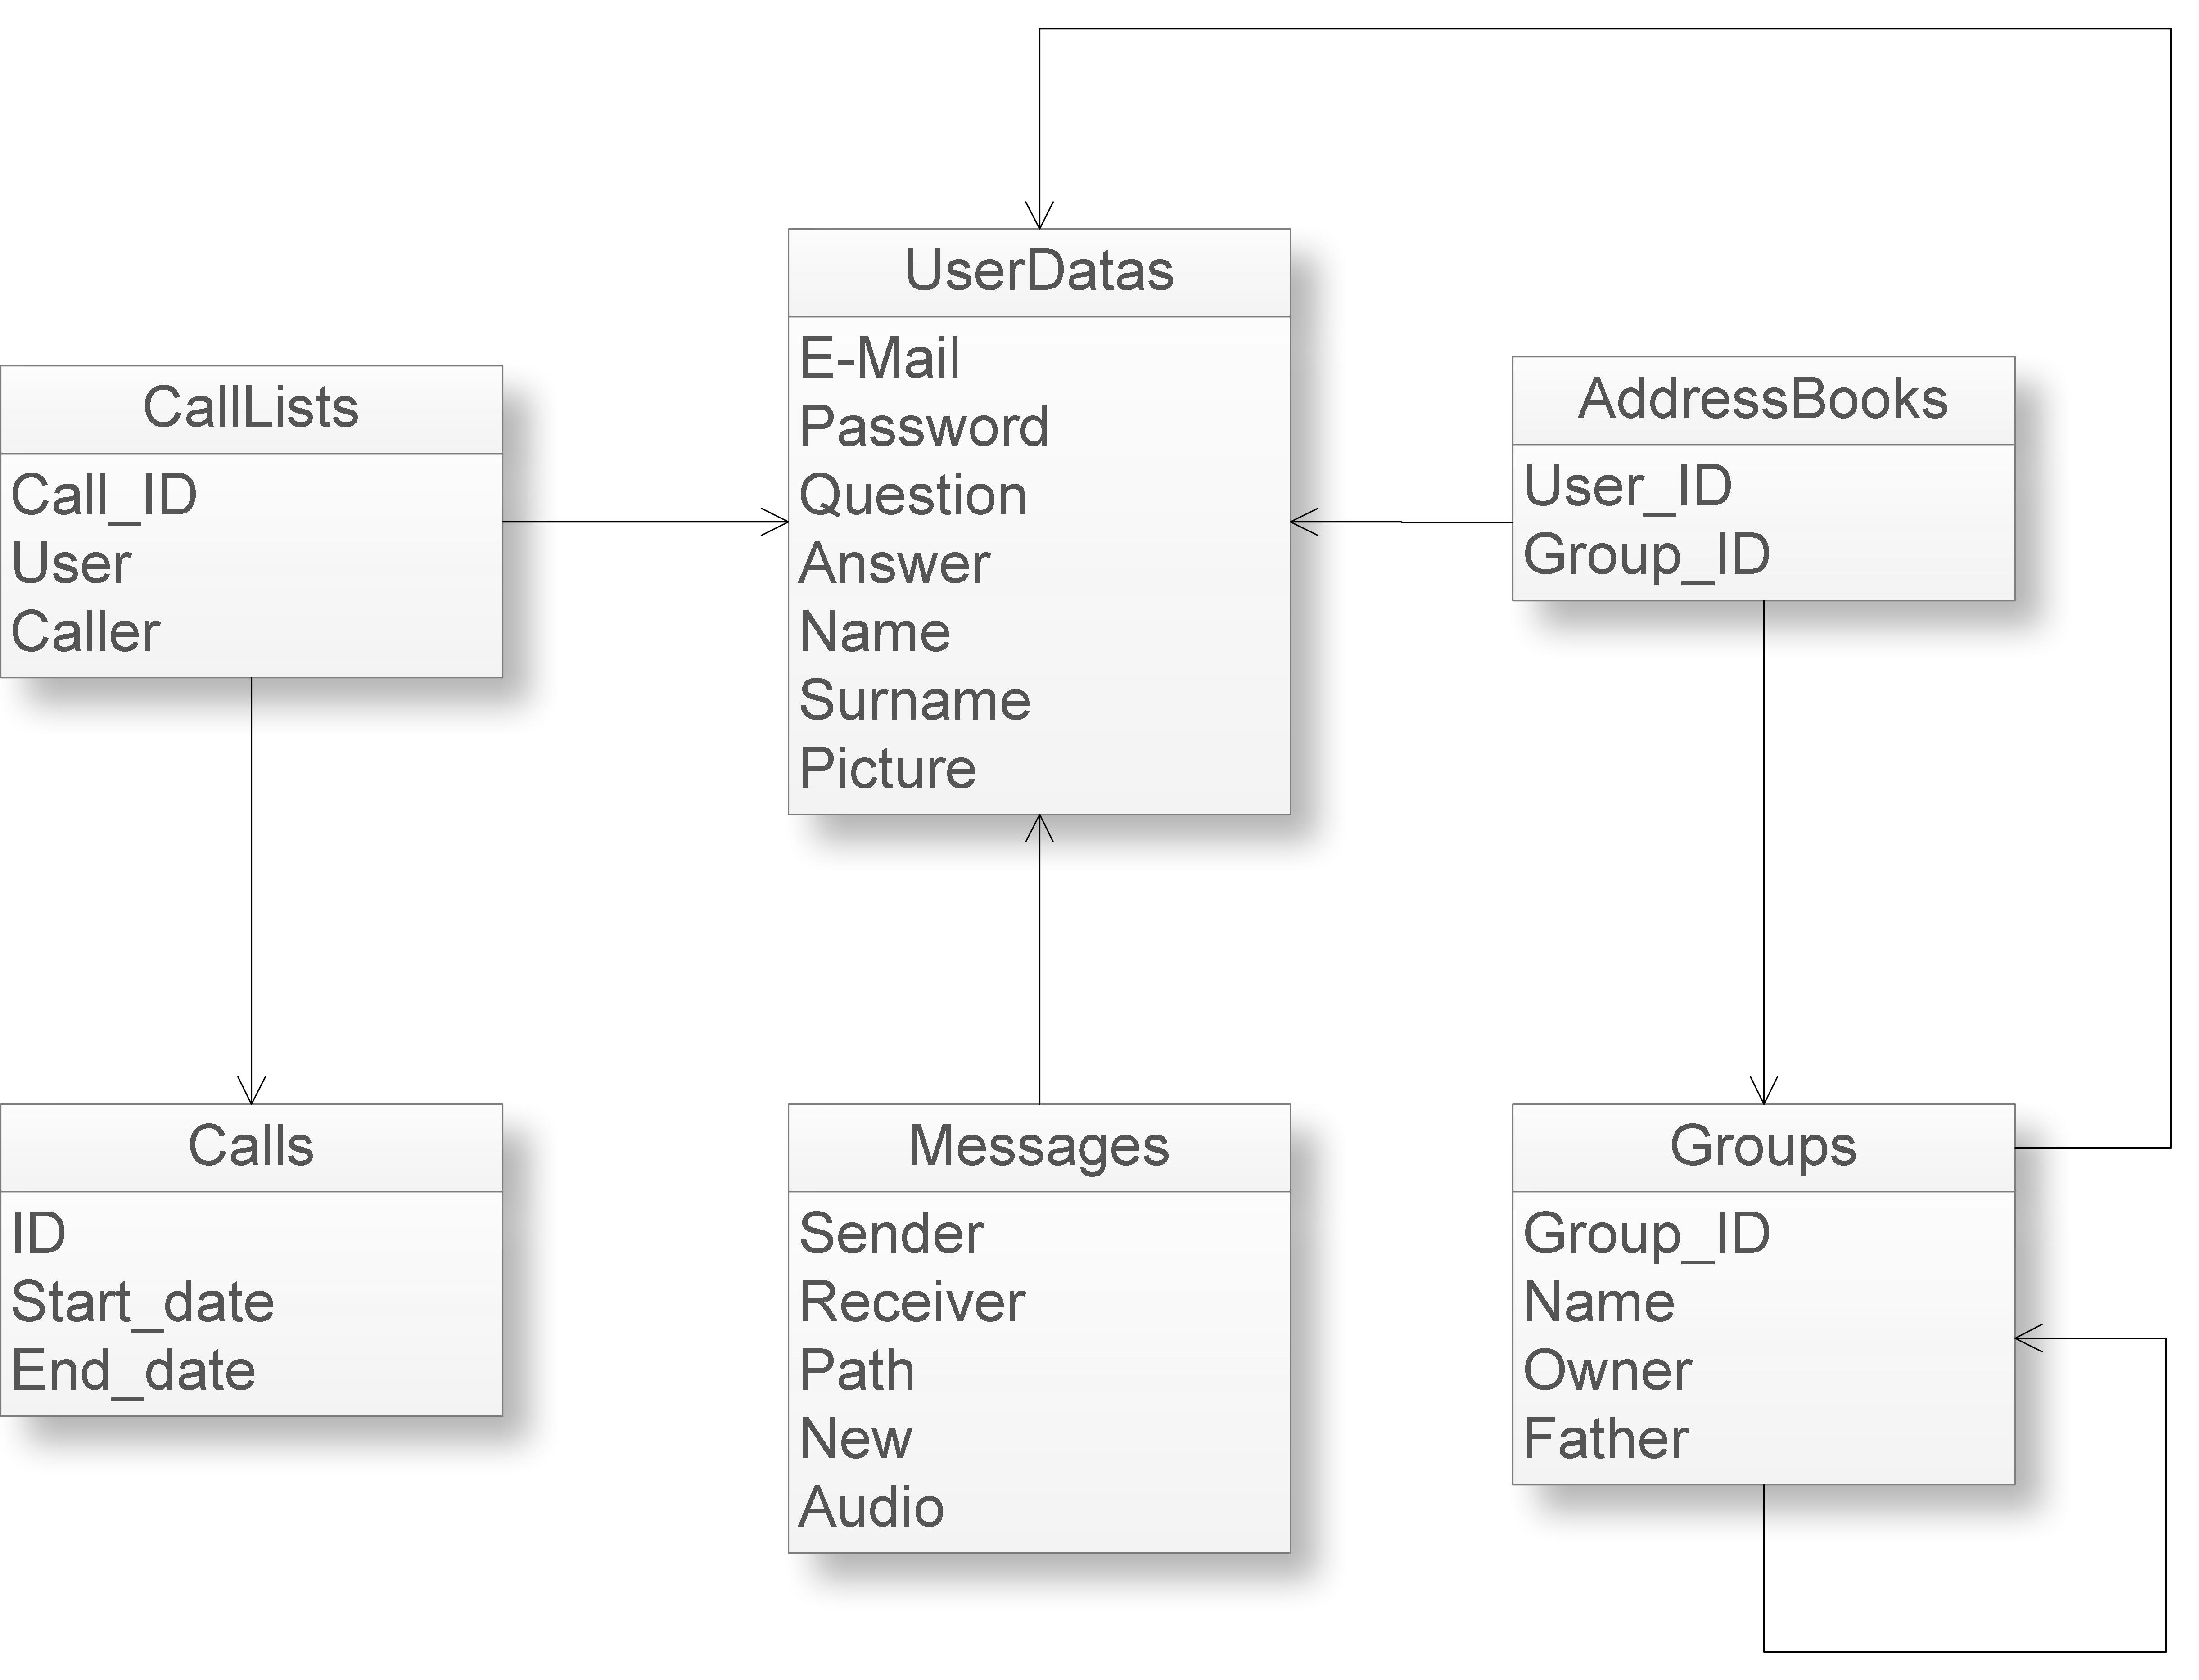
\includegraphics[width=.9\textwidth]{Database_logico}
\caption{Diagramma delle classi - Schema logico Database}\label{fig:database_logico}
\end{center}
\end{figure}

\clearpage

\section{Architettura mytalk.server}
Tale sotto-architettura definisce le specifiche e le funzionalità dell'applicativo lato \underline{server}. In esso saranno definiti i seguenti componenti:
\begin{itemize}[noitemsep,nolistsep]
	\item[-] Gestione Database.
	\item[-] Gestione connessione.
	\item[-] Gestione rubrica.
	\item[-] Gestione stato.
	\item[-] Gestione segreteria.
	\item[-] Façade del server.
\end{itemize}

I componenti sopracitati verranno definiti di seguito. Si sottolinea sin da ora che il \underline{server} è l'unico in grado di comunicare con il \underline{database} su cui regge l'applicativo.

Infine, si fa notare che i nomi di tutte le classi riportate nella sezione sono implicitamente parte del package \texttt{org.softwaresynthesis.mytalk.server} pertanto tale prefisso sarà omesso nella loro denominazione.

\subsection{Componenti evidenziati}

\subsubsection{Gestione database}
\begin{description}
\item{\scshape\bfseries Descrizione:}\\
Gestione Database è il componente che si occupa di rappresentare la struttura del \underline{database} relazionale su cui poggia l'applicativo. Le singole classi in esso definite rappresentano quindi le tabelle del \underline{database}. In termini tecnici le classi interne al componente Gestione database implementa il \underline{design pattern} DAO\@.

Tramite questo componente, il sistema potrà quindi effettuare operazione di lettura e scrittura di entità all'interno del \underline{database}. Le classi che costituiscono il componente dovranno quindi essere dotate di:

\begin{itemize}
	\item metodi get per restituire i singoli attributi dell'istanza;
	\item metodi set per garantire un corretto inserimento dei dati prima di registrare l'istanza nel \underline{database}.
\end{itemize}

Si informa inoltre che le classi di tale componente dovranno interagire con il \underline{framework} Hibernate, al fine di ottenere lo scopo precisato.

\item{\scshape\bfseries Diagramma delle classi:}
\begin{figure}[H]
\begin{center}
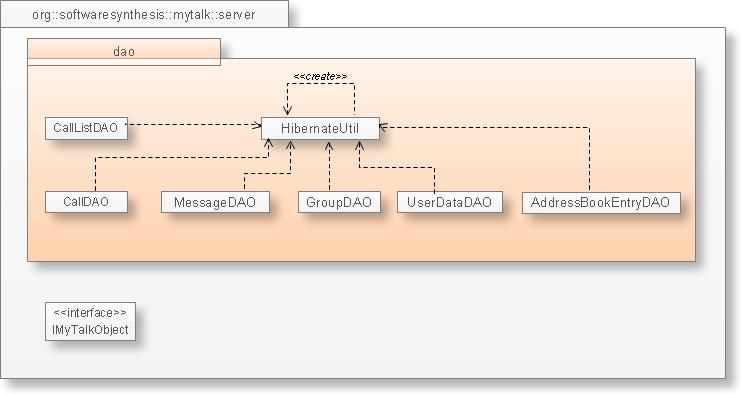
\includegraphics[width=.5\textwidth]{class_gestione_database}
\caption{Diagramma delle classi - Gestione database}\label{fig:gestione_database}
\end{center}
\end{figure}
	
	\item{\scshape\bfseries Classi utilizzate:}
	\begin{itemize}[nolistsep, noitemsep]
	  \item[-] \texttt{dao.AudioMessage}
	  \item[-] \texttt{dao.AudioVideoMessage}
	  \item[-] \texttt{dao.IAudioMessage}
	  \item[-] \texttt{dao.IAudioVideoMessage}
	  \item[-] \texttt{dao.IGroup}
	  \item[-] \texttt{dao.IUserData}
	  \item[-] \texttt{dao.StandardGroup}
	  \item[-] \texttt{dao.StandardUserData}
	\end{itemize}
\end{description}

\subsubsection{Gestione connessione}
\begin{description}
	\item{\scshape\bfseries Descrizione:}\\
Tale componente ingloba le classi destinate a stabilire le routine di connessione. A tal fine è stata definita l'interfaccia di una classe Singleton \texttt{connection.ICommunicationHandler}, implementata da \texttt{connection.StandardCommunicationHandler} che ha il compito di creare oggetti connessione.

Le specifiche di tali oggetti sono descritte dall'interfaccia \texttt{connection.IConnection}, con la relativa implementazione \texttt{connection.WebRTCInfo}.
	\item{\scshape\bfseries Diagramma delle classi:}
	\begin{figure}[H]
\begin{center}
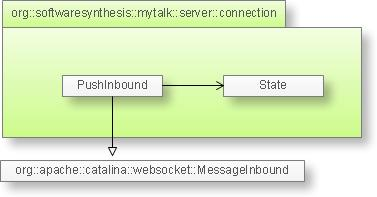
\includegraphics[width=.8\textwidth]{class_gestione_connessione}
\caption{Diagramma delle classi - Gestione connessione}\label{fig:gestione_connessione}
\end{center}
\end{figure}
	
	\item{\scshape\bfseries Classi utilizzate:}
	\begin{itemize}[nolistsep, noitemsep]
	  \item[-] \texttt{connection.ICommunicationHandler}
	  \item[-] \texttt{connection.StandardCommunicationHandler}
	  \item[-] \texttt{connection.IConnection}
	  \item[-] \texttt{connection.WebRTCInfo}
	\end{itemize}
\end{description}

\subsubsection{Gestione rubrica}
\begin{description}
	\item{\scshape\bfseries Descrizione:}\\
La rubrica è organizzata in gruppi e sono previste due categorie di default: la \textit{blacklist} e la \textit{whitelist}.

L'utente può aggiungere ulteriori gruppi in base alle sue esigenze ma esclusivamente all'interno della \textit{whitelist}. Per trattare in maniera omogenea i gruppi di contatti e i singoli contatti si è utilizzato il \underline{design pattern} Composite.

In particolare, \texttt{abook.IContact} rappresenta l'interfaccia principale comune a ogni tipologia di contatto e viene estesa dalle due interfacce \texttt{dao.IUserData} e \texttt{dao.IGroup}.

Il componente comprende anche l'interfaccia \texttt{abook.IAddressBook} e la relativa implementazione \texttt{abook.AddressBook}. Nell'implementazione specificata \texttt{abook.Addressbook} vincola il sistema a garantire che ogni utente abbia i due gruppi di default sopra descritti, come richiesto dai requisiti.

Infine, la classe \texttt{abook.UserDataProxy} viene utilizzata come proxy per lo scambio di dati fra la sotto-architettura \underline{server} e la sotto-architettura clientpresenter.
	\item{\scshape\bfseries Diagramma delle classi:}
	\begin{figure}[H]
\begin{center}
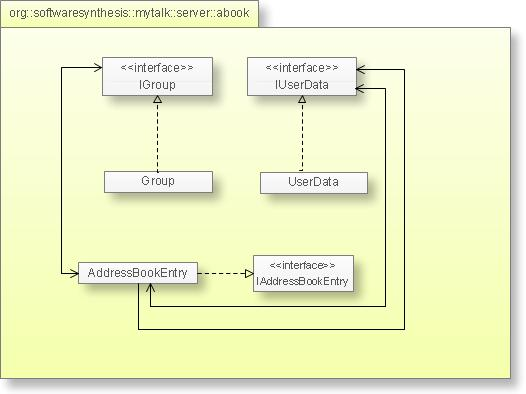
\includegraphics[width=.8\textwidth]{class_gestione_rubrica}
\caption{Diagramma delle classi - Gestione rubrica}\label{fig:gestione_rubrica}
\end{center}
\end{figure}
	
	\item{\scshape\bfseries Classi utilizzate:}\\
	\begin{itemize}[nolistsep, noitemsep]
	  \item[-] \texttt{abook.AddressBook}
	  \item[-] \texttt{abook.IAddressBook}
	  \item[-] \texttt{abook.IContact}
	  \item[-] \texttt{abook.UserDataProxy}
	  \item[-] \texttt{dao.IGroup}
	  \item[-] \texttt{dao.IUserData}
	\end{itemize}
\end{description}

\subsubsection{Gestione stato}
\begin{description}
	\item{\scshape\bfseries Descrizione:}\\
Le classi di tale componente sono utilizzate per gestire lo stato degli utenti, permettendo un comportamento diverso delle istanze di \texttt{dao.StandardUserData} a seconda dello stato in cui si trova l'utente corrispondente. Gli stati possibili sono in prima istanza ``online'' e ``offline'', rappresentati dalle classi \texttt{state.StateOnline} e \texttt{state.StateOffline} rispettivamente.

Gli utenti che si trovano nello stato online possono trovarsi in due situazioni: ``occupato'' o ``disponibile'', rappresentati a loro volta dalle classi \texttt{state.StateOccupied} e \texttt{state.StateAvailable}.

Se l'utente è impegnato in una conversazione con uno o più utenti, allora lo stato in cui si trova è ``occupato''. Tuttavia, un utente può anche impostare manualmente il proprio stato ad ``occupato'' anche per segnalare di non essere disponibile a ricevere chiamate in ingresso.
	
La chiamata viene inoltre trattata in modo differente a seconda che l'utente si trovi nello stato ``disponibile'' o ``occupato''/``offline'', dal momento che nel primo caso la chiamata va a buon fine mentre nel secondo verrà attivato il meccanismo di segreteria telefonica.
	
Inoltre, i cambiamenti di stato vengono notificati a tutti gli utenti presenti in rubrica tali che si trovano nello stato online.
	\item{\scshape\bfseries Diagramma delle classi:}
	\begin{figure}[H]
\begin{center}
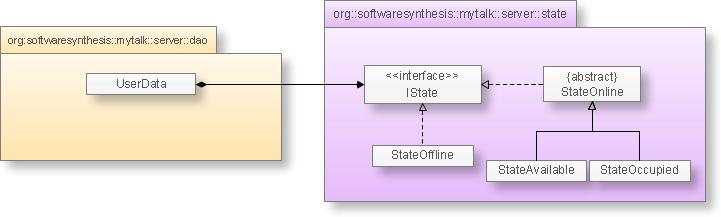
\includegraphics[width=.9\textwidth]{class_gestione_stato}
\caption{Diagramma delle classi - Gestione stato}\label{fig:gestione_stato}
\end{center}
\end{figure}
	
	\item{\scshape\bfseries Classi utilizzate:}\\ 
	\begin{itemize}[noitemsep,nolistsep]
		\item[-] \texttt{dao.StandardUserData}
	    \item[-] \texttt{state.IState}
	    \item[-] \texttt{state.StateAvailable}
	    \item[-] \texttt{state.StateOccupied}
	    \item[-] \texttt{state.StateOffline}
	    \item[-] \texttt{state.StateOnline}
	\end{itemize}
\end{description}

\subsubsection{Gestione segreteria}
\begin{description}
	\item{\scshape\bfseries Descrizione:}\\
Il sistema di segreteria telefonica corrisponde all'interfaccia \texttt{message.IMessageBox} e alla relativa implementazione \texttt{message.StandardMessageBox} che permettono un accesso centralizzato all'insieme di messaggi che un determinato utente ha ricevuto.

I messaggi audio e audio/video sul \underline{server} sono rappresentati dalle classi \texttt{dao.IAudioMessage} (implementata da \texttt{dao.AudioMessage}) e \texttt{dao.IAudioVideoMessage} (implementata da \texttt{dao.AudioVideoMessage}) rispettivamente.

L'onere di caricare in memoria e gestire l'interno contenuto del messaggio è posticipato al momento di effettiva necessità mediante l'utilizzo dei \textit{virtual proxy} corrispondenti alle classi \texttt{message.AudioMessageProxy} e \texttt{message.AudioVideoMessageProxy}.
	\item{\scshape\bfseries Diagramma delle classi:}
\begin{figure}[H]
\begin{center}
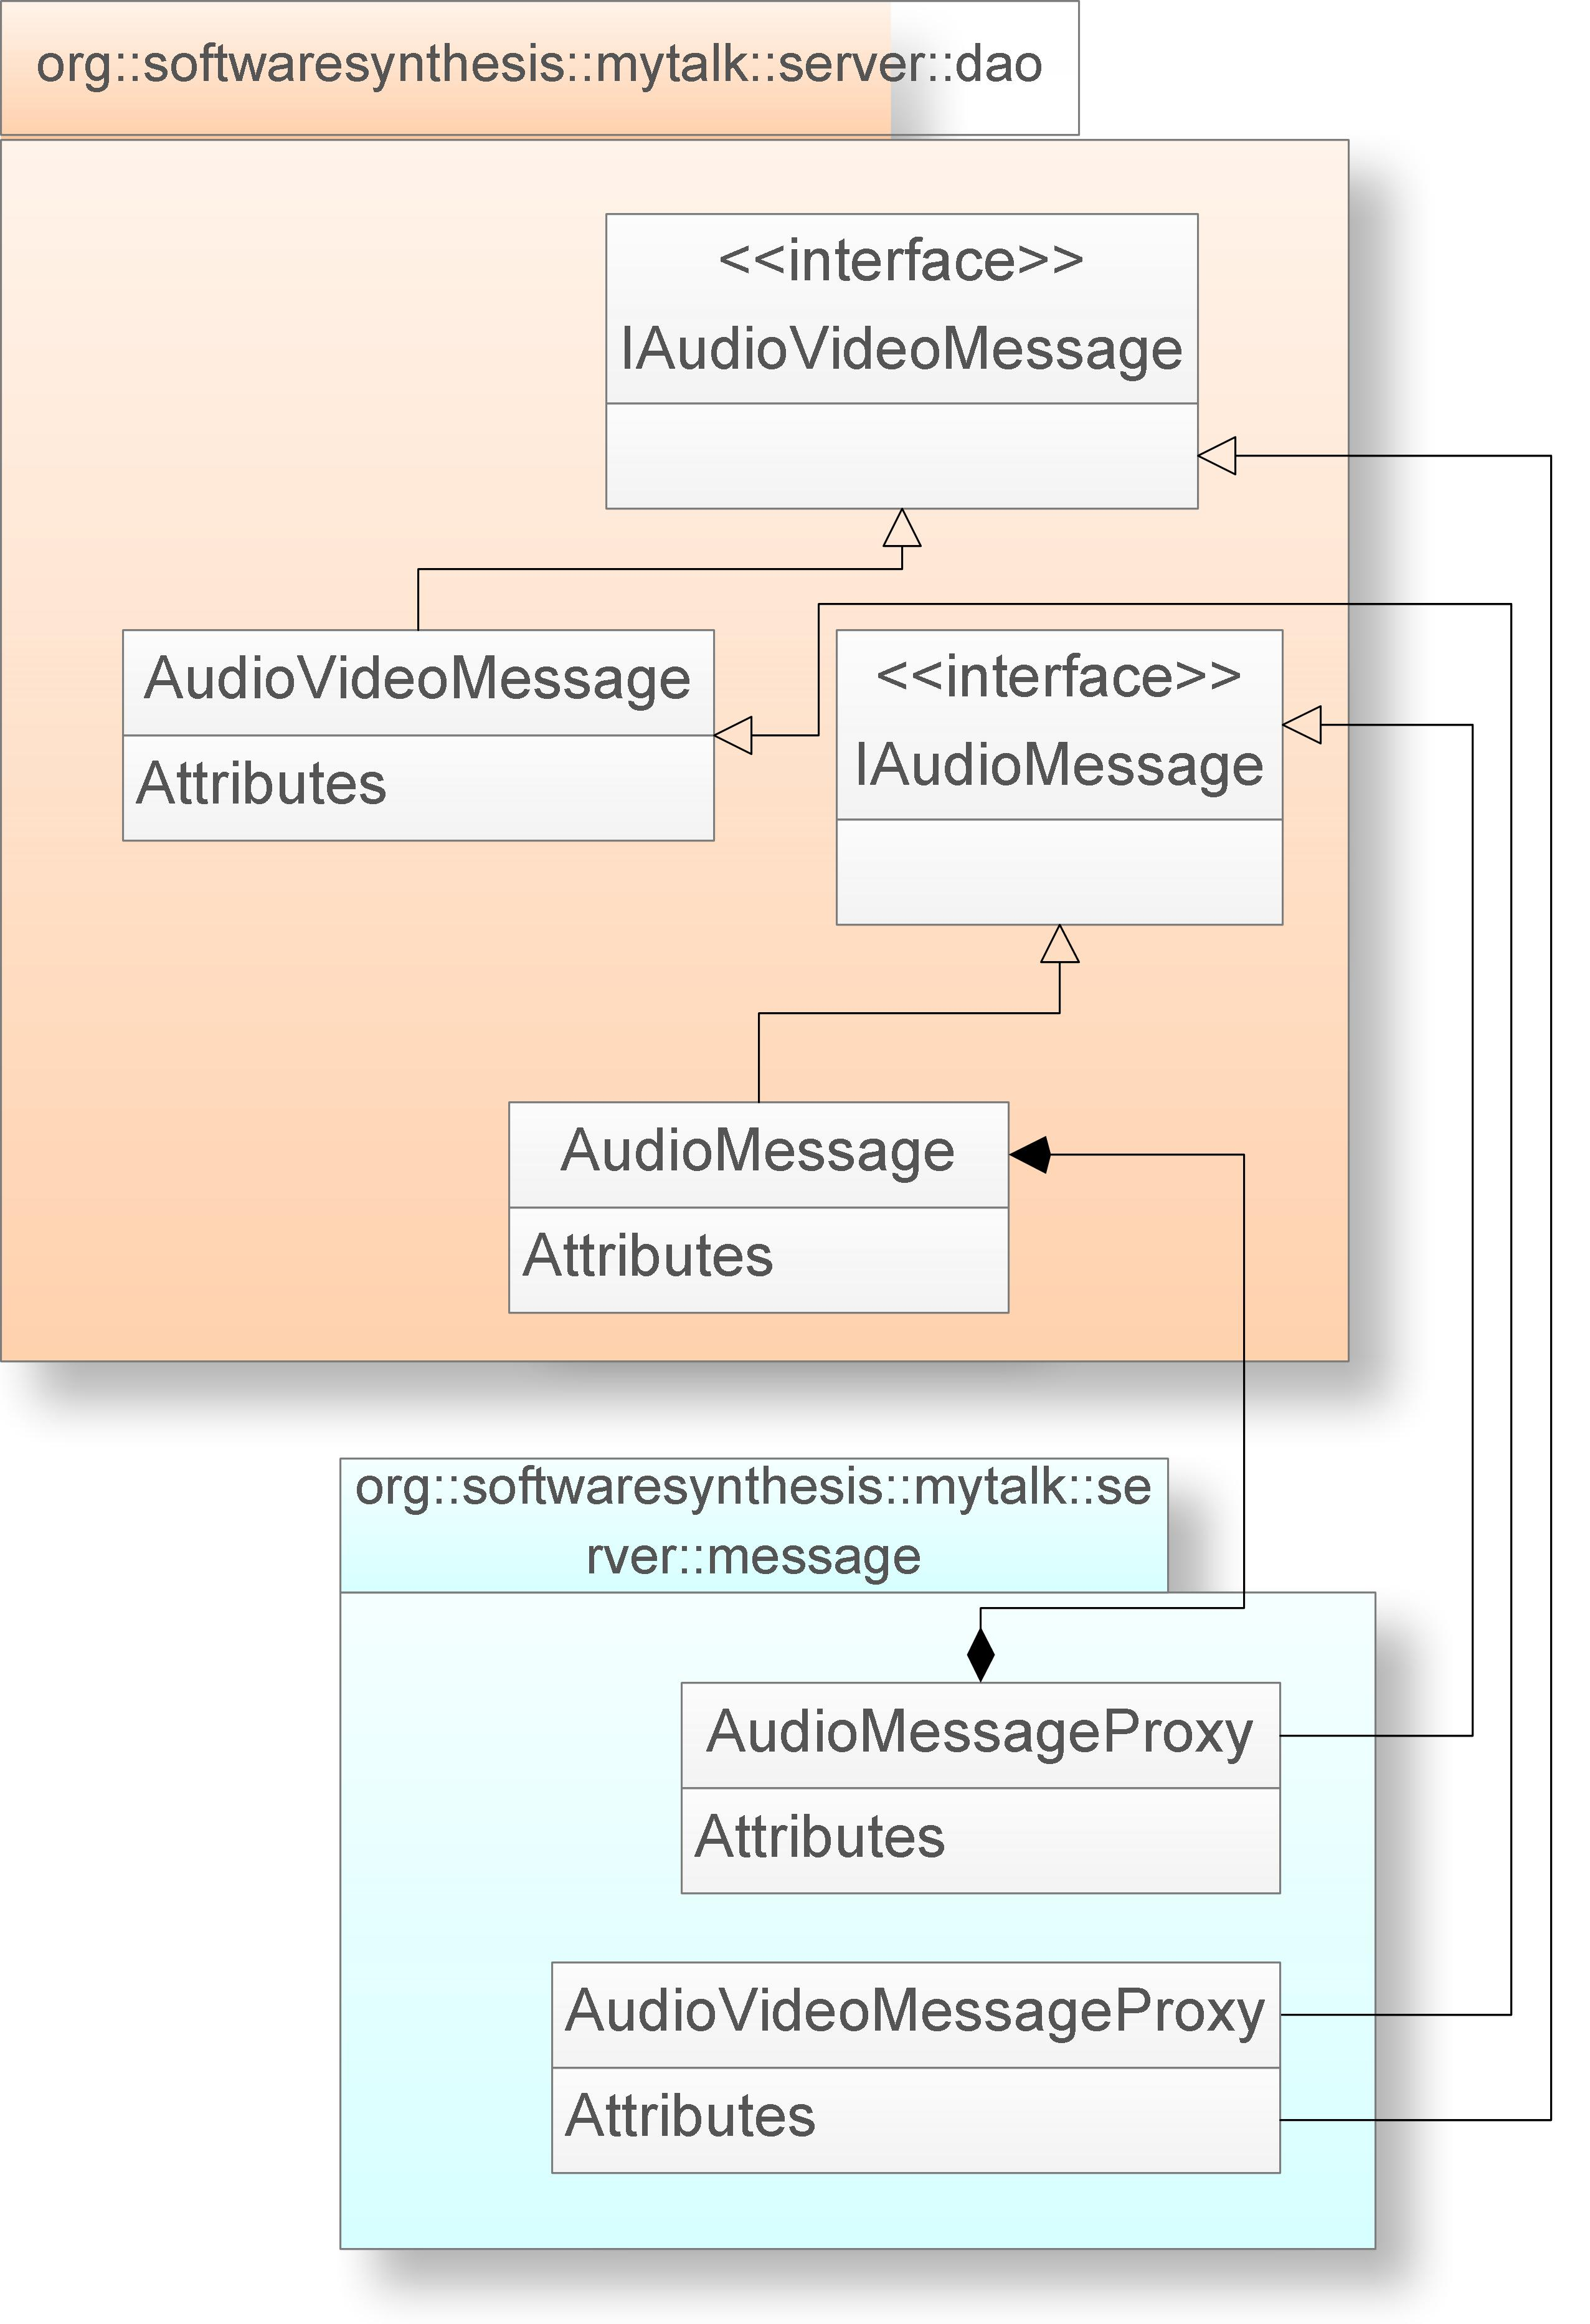
\includegraphics[width=.6\textwidth]{class_gestione_segreteria}
\caption{Diagramma delle classi - Gestione segreteria}\label{fig:gestione_segreteria}
\end{center}
\end{figure}	
	
	\item{\scshape\bfseries Classi utilizzate:}
	\begin{itemize}[noitemsep,nolistsep]
	  \item[-] \texttt{dao.AudioMessage}
	  \item[-] \texttt{dao.AudioVideoMessage}
	  \item[-] \texttt{dao.IAudioMessage}
	  \item[-] \texttt{dao.IAudioVideoMessage}
	  \item[-] \texttt{message.AudioMessageProxy}
	  \item[-] \texttt{message.AudioVideoMessageProxy}
	\end{itemize}
\end{description}

\subsubsection{Façade del server}
\begin{description}
	\item{\scshape\bfseries Descrizione:}\\
L'interfaccia \texttt{IServerFacade} e la relativa implementazione \texttt{StandardServerFacade}, nella quale si è scelto di applicare il \underline{design pattern} Singleton, forniscono una sorta di interfaccia alle funzionalità offerte dalla sotto-architettura \underline{server} ai componenti che risiedono nel \underline{client}.

Le funzionalità esposte consentono di gestire i messaggi presenti in segreteria, le richieste di comunicazione con altri utenti il login/registrazione degli utenti.
	\item{\scshape\bfseries Diagramma delle classi:}
\begin{figure}[H]
\begin{center}
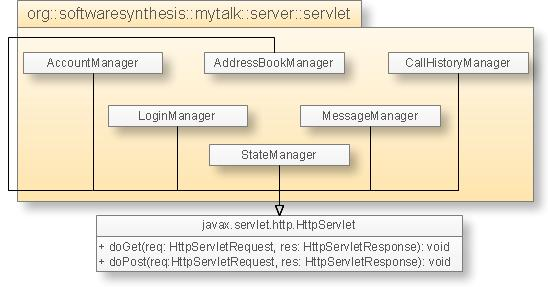
\includegraphics[width=.8\textwidth]{class_facade_server}
\caption{Diagramma delle classi - Façade del server}\label{fig:facade_server}
\end{center}
\end{figure}	
	
	\item{\scshape\bfseries Classi utilizzate:}\\
	\begin{itemize}[noitemsep,nolistsep]
	  \item[-] \texttt{IServerFacade}
	  \item[-] \texttt{StandardServerFacade}
	\end{itemize}
\end{description}


\subsection{Diagramma delle classi}
\begin{figure}[H]
\begin{center}
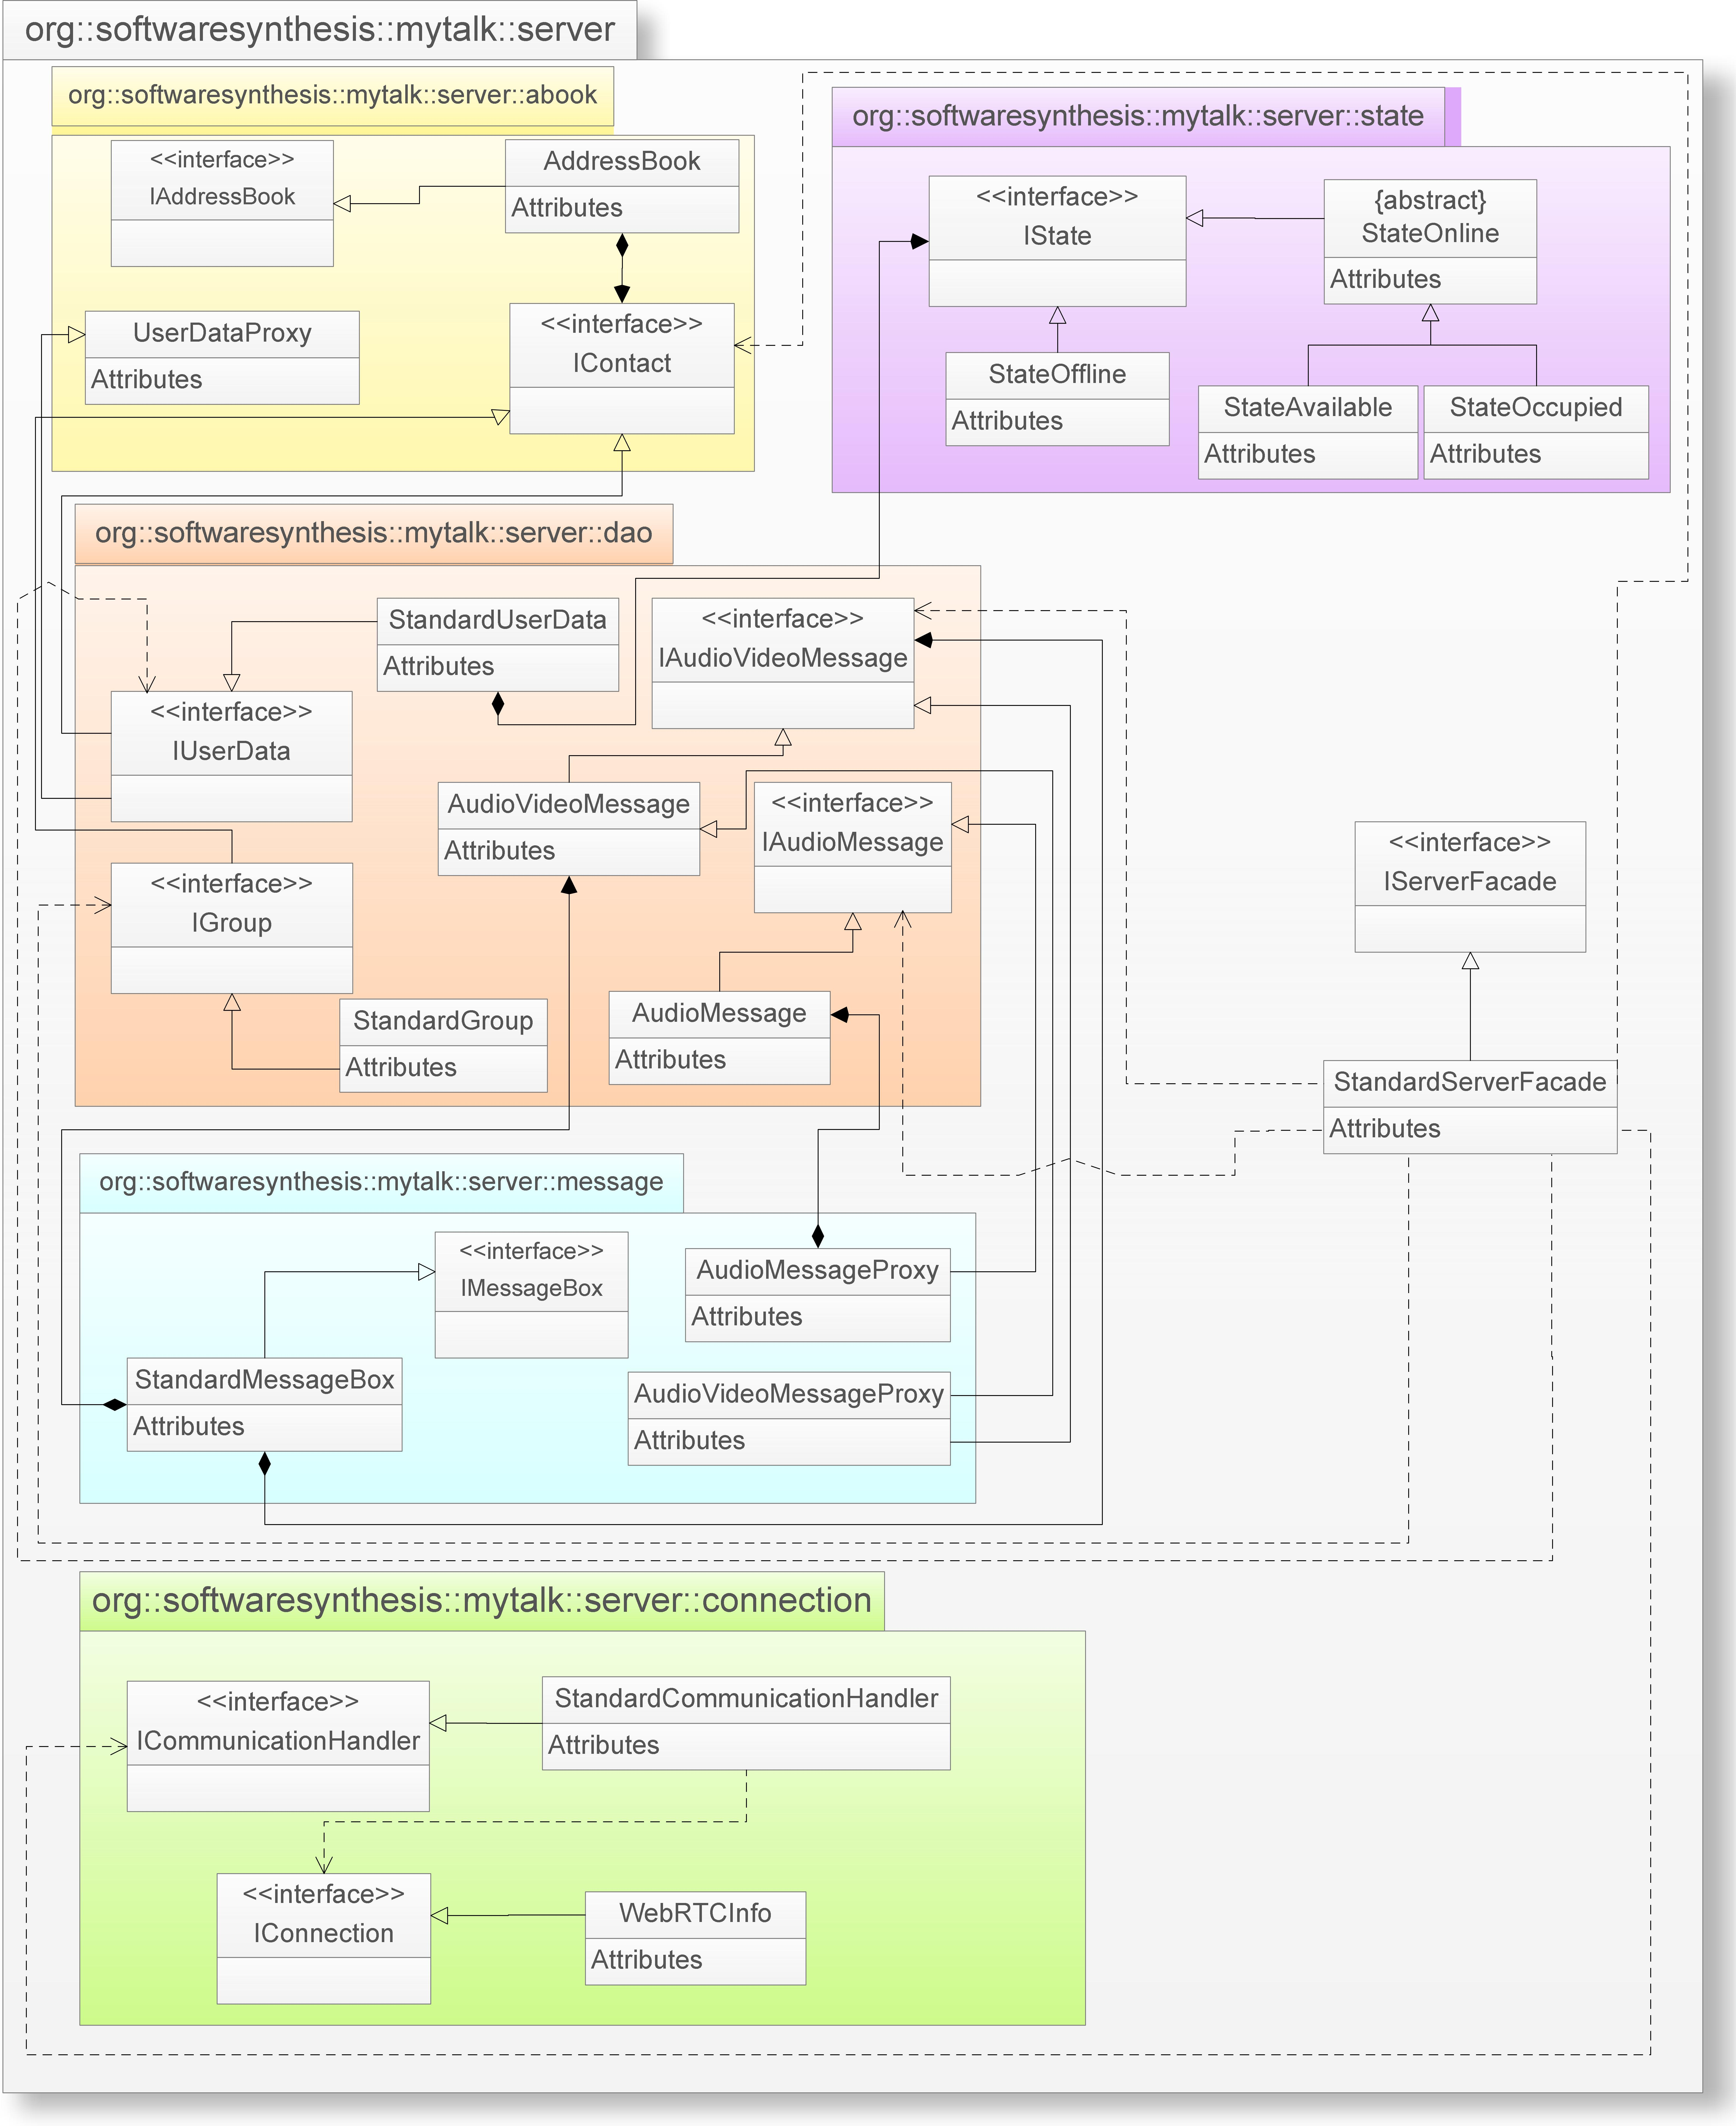
\includegraphics[width=1\textwidth]{server_generale}
\caption{Diagramma delle classi - Architettura mytalk.server}\label{fig:server_generale}
\end{center}
\end{figure}
\clearpage

\section{Architettura mytalk.clientpresenter}
La sotto-architettura clientpresenter, nasce con lo scopo di imporre una separazione tra la logica di gestione di un \underline{client} e l'interfaccia grafica usata da quest'ultimo.

Tale considerazione è conforme a l'utilizzo del \underline{design pattern} MVP, già citato nella sezione ``Design pattern'', e alla quale rimandiamo per le specifiche tecniche del medesimo.

La sotto-architettura clientpresenter è per l'appunto la parte ``presenter'' dell'applicativo. I componenti che lo costituiscono devono quindi garantire una logica stabile di comunicazione con il \underline{server}. Essi dovranno anche stabilire le procedure per interrogare il \underline{server} (attraverso il suo façade) al fine di ottenere:
\begin{itemize}
	\item i vari dati contenuti nel \underline{database};
	\item le ``informazioni'' necessarie per stabilire una connessione \underline{client}-\underline{client}.
\end{itemize}

In sintesi la sotto-architettura clientpresenter dispone dei seguenti componenti:
\begin{itemize}[noitemsep,nolistsep]
	\item[-] Gestione comunicazione;
	\item[-] Façade del presenter.
\end{itemize}
Si rimanda alla sottosezione successiva per maggiori dettagli.

Si fa notare che i nomi di tutte le classi riportate nella sezione sono implicitamente parte del package \texttt{org.softwaresynthesis.mytalk.clientpresenter} pertanto tale prefisso sarà omesso nella loro denominazione.

\subsection{Logica di rete}
La rete che viene a crearsi sotto l'architettura di \caName{} è suddivisa in ``comunicazioni'', ovvero gruppi di due o più utenti che comunicano tra di loro. Ogni comunicazione è formata dalle singole ``connessioni'' tra i vari \underline{client}.

Questo capitolo serve a spiegare quale è la logica che governa la rete. Iniziamo definendo i tipi di \underline{client} che la popolano.
\begin{description}
	\item{\scshape\bfseries Nodo}\\
	Il Nodo è rappresentato da un semplice \underline{client} che si trova all'interno di una comunicazione e che ha una unica connessione attiva verso un altro \underline{client}.
	\item{\scshape\bfseries Supernodo}\\
	Il Supernodo è un \underline{client} con funzione di \underline{server}. È usato nelle comunicazioni tra tre o più utenti per smistare le connessioni di tutti facendosi carico del traffico dei \underline{client}.
\end{description}

Vediamo nel dettaglio come avviene una comunicazione. Essa nasce sempre tra due utenti, nel momento in cui uno desidera iniziarla effettua una richiesta verso il \underline{server} che la inoltra al destinatario.
La comunicazione nasce così come un'unica connessione tra due \underline{client} in modalità \underline{peer-to-peer} dove entrambi gli utenti hanno il ruolo di Nodo. Una comunicazione potrà iniziare solo attraverso tale metodologia, in quanto non vengono aperte comunicazioni iniziali tra più di due utenti.

Da questa situazione uno dei due utenti può richiederne l'aggiunta di un ulteriore soggetto. Dopo questa richiesta, il Nodo che la ha eseguita diventa un Supernodo con attive sia la connessione con il vecchio Nodo sia quella con il nuovo Nodo appena aggiunto.

Questa operazione crea una connessione fra tre Nodi estendibile dal Supernodo e dagli altri Nodi attraverso una richiesta al Supernodo stesso. 
%Solo il Supernodo può richiedere nuove connessioni al Server. Con ulteriori richieste i nuovi nodi si collegano al Supernodo con una connessione estendendo la comunicazione.

Ogni Nodo può togliersi dalla comunicazione chiudendo la connessione con il Supernodo. Se è il Supernodo stesso a volersi togliere dalla comunicazione, l'intera comunicazione cade e tutti gli utenti vendono disconnessi.

\subsubsection{L'idea iniziale}
La logica di gestione della rete scelta dal team può rendere poco stabile le comunicazioni. Tale problematica è stata analizzata a lungo, e al fine di rendere le comunicazioni più stabili e solide era stata presa in considerazione un ulteriore soluzione alternativa sempre basata sul modello concettuale di Nodi e Supernodi, tuttavia è stata scartata dopo una breve analisi preliminare.

La differenza principale di tale soluzione rispetto a quella adottata è nella gestione dinamica del Supernodo, che viene scelto in base alla sua capacità di banda e alla possibilità di mantenere attive, con la massima qualità, tutte le connessioni con i Nodi della comunicazione.

Questa soluzione avrebbe richiesto un test di qualità della rete per ogni Nodo verso il nuovo possibile Supernodo, operazione di difficile progettazione e con complessità elevata, pari a $\omega(n-1)$ con n Nodi attivi nella comunicazione.

Al fine di garantire sempre la migliore qualità di connessione era stata presa inoltre in considerazione l'idea di controllare periodicamente la qualità del Supernodo e degli altri Nodi in modo da sostituire il Supernodo se necessario. Purtroppo anche questa soluzione richiederebbe dei calcoli di complessità $\omega(n*n-1)$ con n Nodi attivi nella comunicazione.

Con una corretta implementazione questa soluzione avrebbe permesso una migliore qualità del prodotto \caName, il gruppo ha tuttavia optato per la prima implementazione presentata in quanto le risorse disponibili non erano sufficienti per terminare la seconda.

\subsection{Componenti evidenziati}

\subsubsection{Gestione comunicazione}
\begin{description}
	\item{\scshape\bfseries Descrizione:}\\
È il componente che definisce i \underline{client} con cui sta comunicando o con cui desidera comunicare l'utente. Tale componente è costituito da un'interfaccia \texttt{clientpresenter.IClient} che rappresenta un modello di \underline{client} con cui interagire (possibilità di stabilire una connessione, possibilità di
estendere una comunicazione e possibilità di verificare se il \underline{client} è Supernodo).

In pratica nel momento in cui l'utente A desidera stabilire una comunicazione con l'utente B, questi si farà restituire dal \underline{server} le informazioni necessarie. Con tali informazioni, quindi, sarà creata un istanza di \texttt{clientpresenter.StandardClient} (implementazione dell'interfaccia \texttt{clientpresenter.IClient}), dalla quale potrà essere abilitata la comunicazione.
	\item{\scshape\bfseries Diagramma delle classi:}
	\begin{figure}[H]
\begin{center}
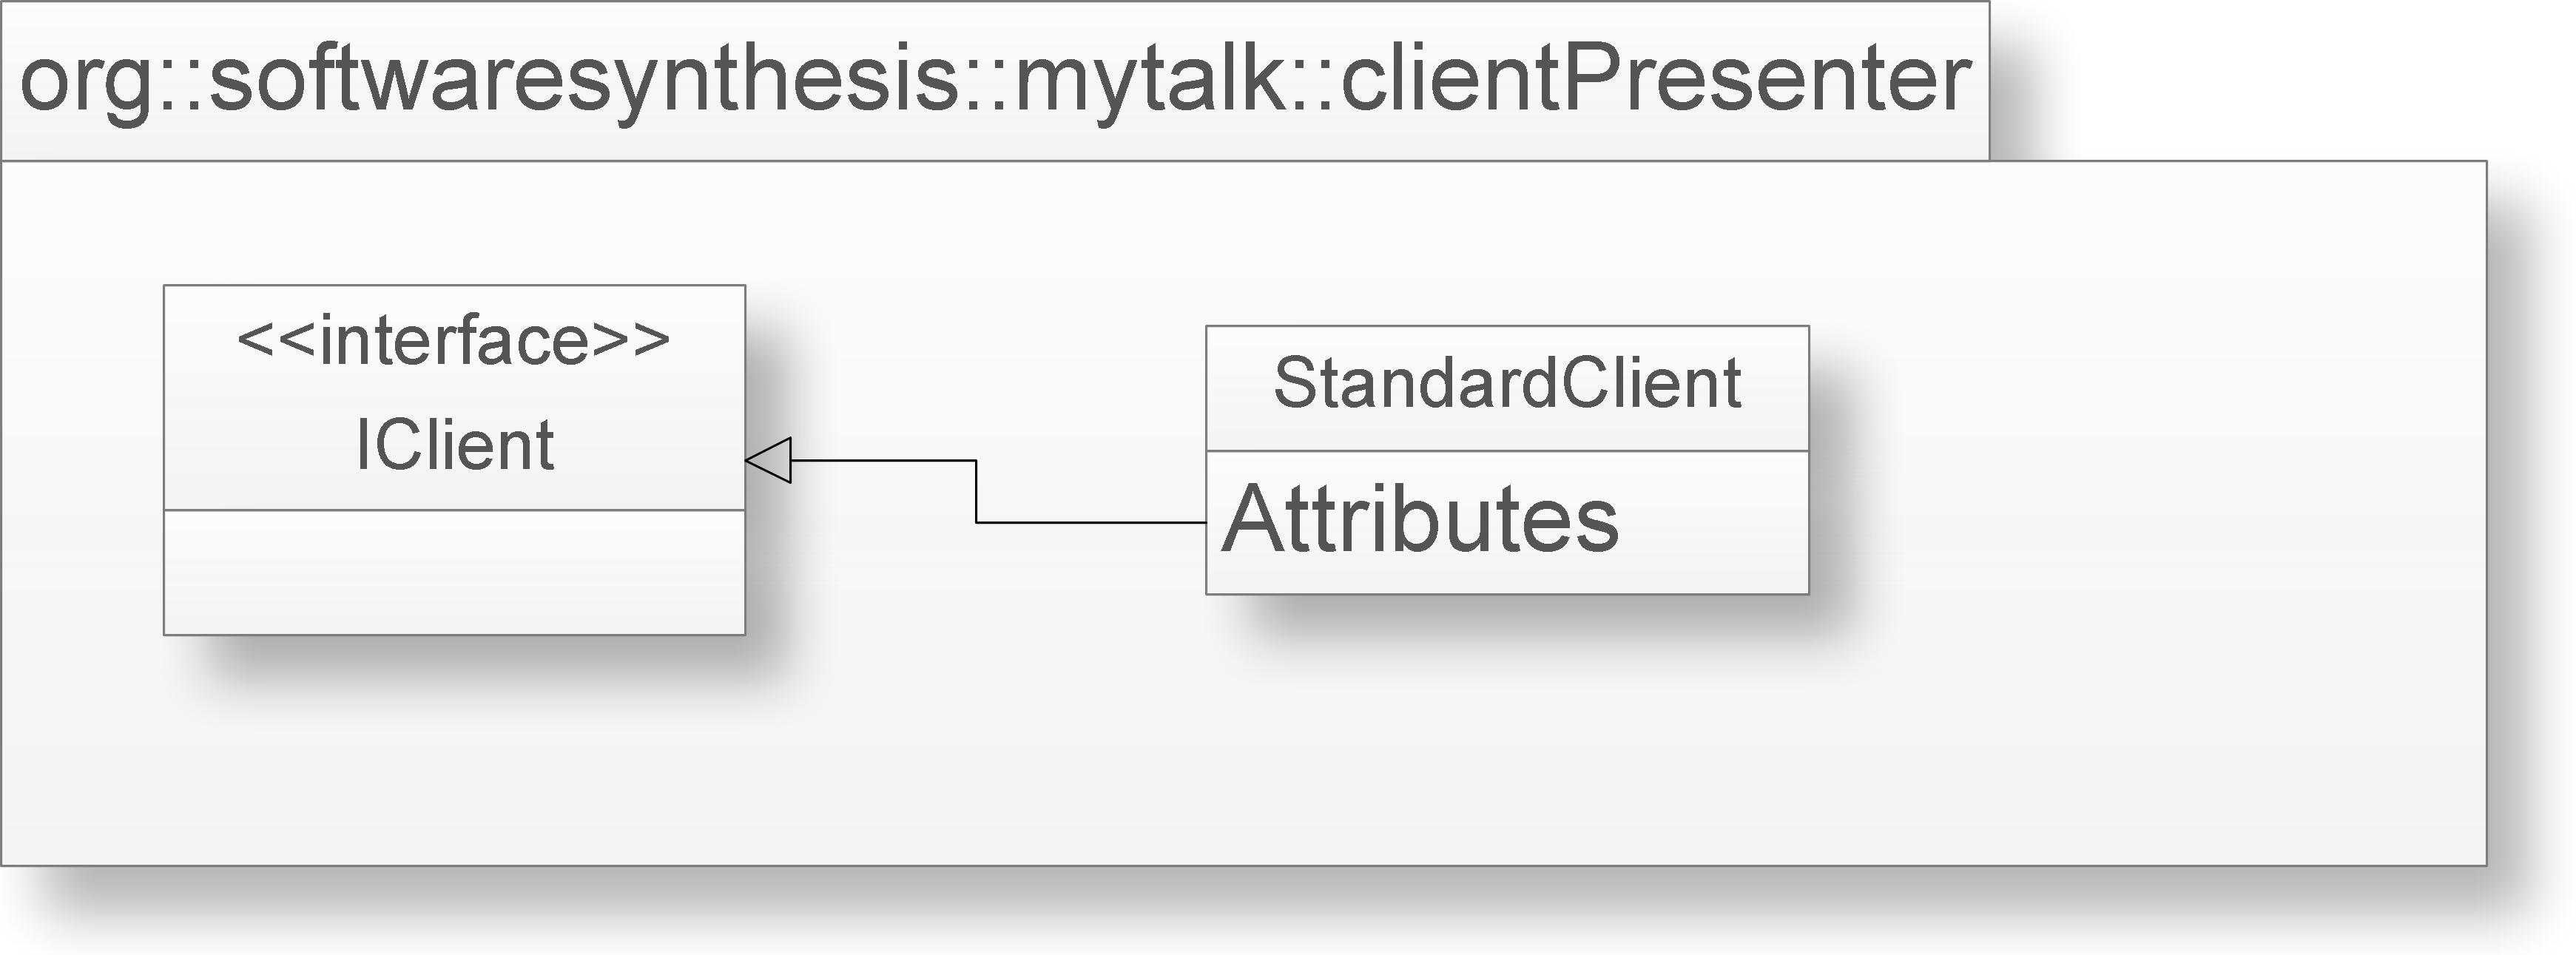
\includegraphics[width=.8\textwidth]{gestione_comunicazione}
\caption{Diagramma delle classi - Gestione comunicazione}\label{fig:gestione_comunicazione}
\end{center}
\end{figure}
	\item{\scshape\bfseries Classi utilizzate:} 
	\begin{itemize}[noitemsep,nolistsep]
		\item[-] \texttt{IClient}
		\item[-] \texttt{StandardClient}
	\end{itemize}  
\end{description}

\subsubsection{Façade del presenter}
\begin{description}
	\item{\scshape\bfseries Descrizione:}\\
Rappresenta l'interfaccia d'accesso verso la sotto-architettura clientpresenter. Tale componente svincola l'interfaccia grafica dal dover conoscere l'esatta sequenza di chiamata dei metodi per portare a conseguimento una determinata procedura.

I metodi del componente Façade del presenter hanno la cognizione dell'iter di chiamate a metodo per portare a termine correttamente la procedura. Il componente in esame richiede la definizione di un'interfaccia e una sua implementazione standard. Rimandiamo a tali classi per un approfondimento sul comportamento da seguire.
	\item{\scshape\bfseries Diagramma delle classi:}
\begin{figure}[H]
\begin{center}
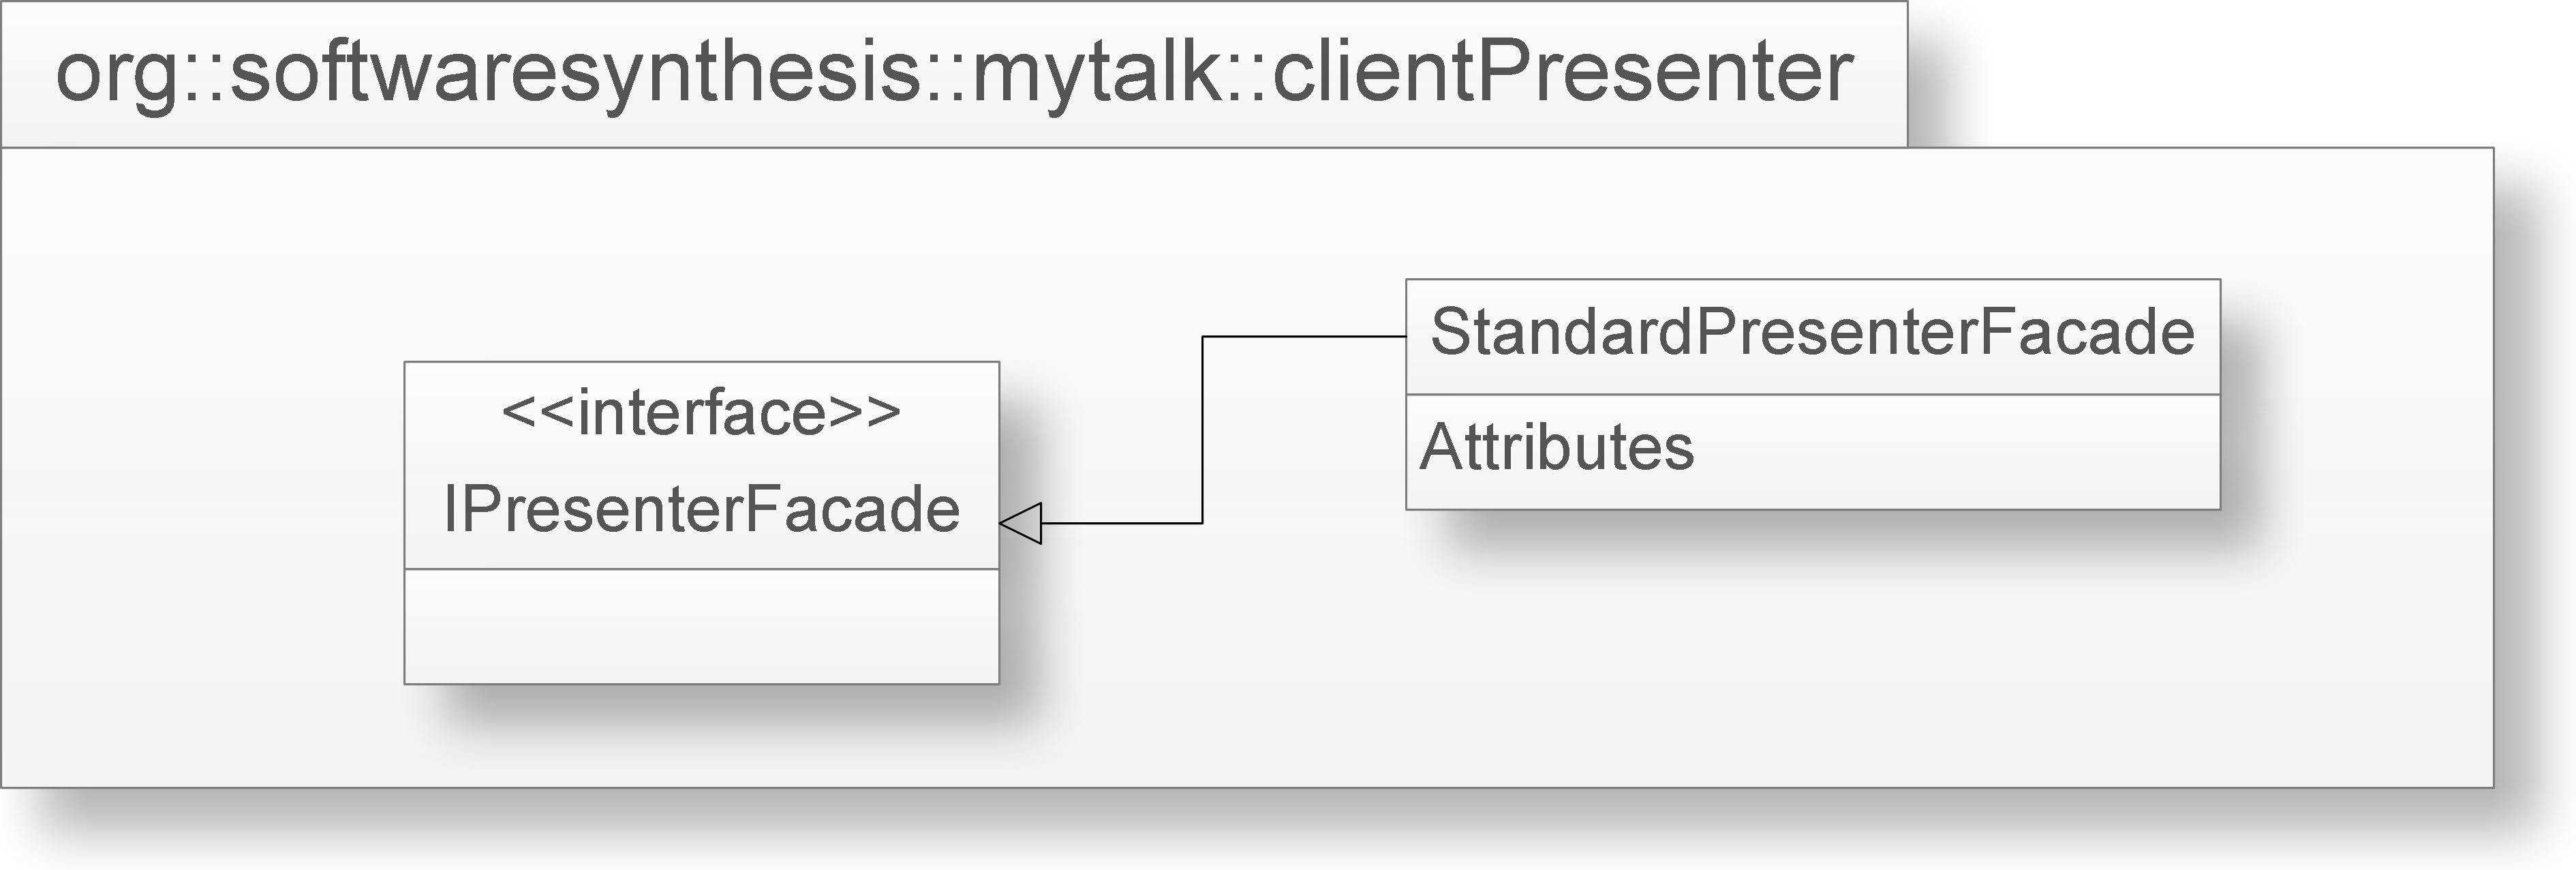
\includegraphics[width=.8\textwidth]{facade_presenter}
\caption{Diagramma delle classi - Façade del presenter}\label{fig:facade_presenter}
\end{center}
\end{figure}
	\item{\scshape\bfseries Classi utilizzate:} 
	\begin{itemize}[noitemsep,nolistsep]
		\item[-] \texttt{IPresenterFacade}
		\item[-] \texttt{StandardPresenterFacade}
	\end{itemize}
\end{description}

\subsection{Diagramma delle classi}
\begin{figure}[H]
\begin{center}
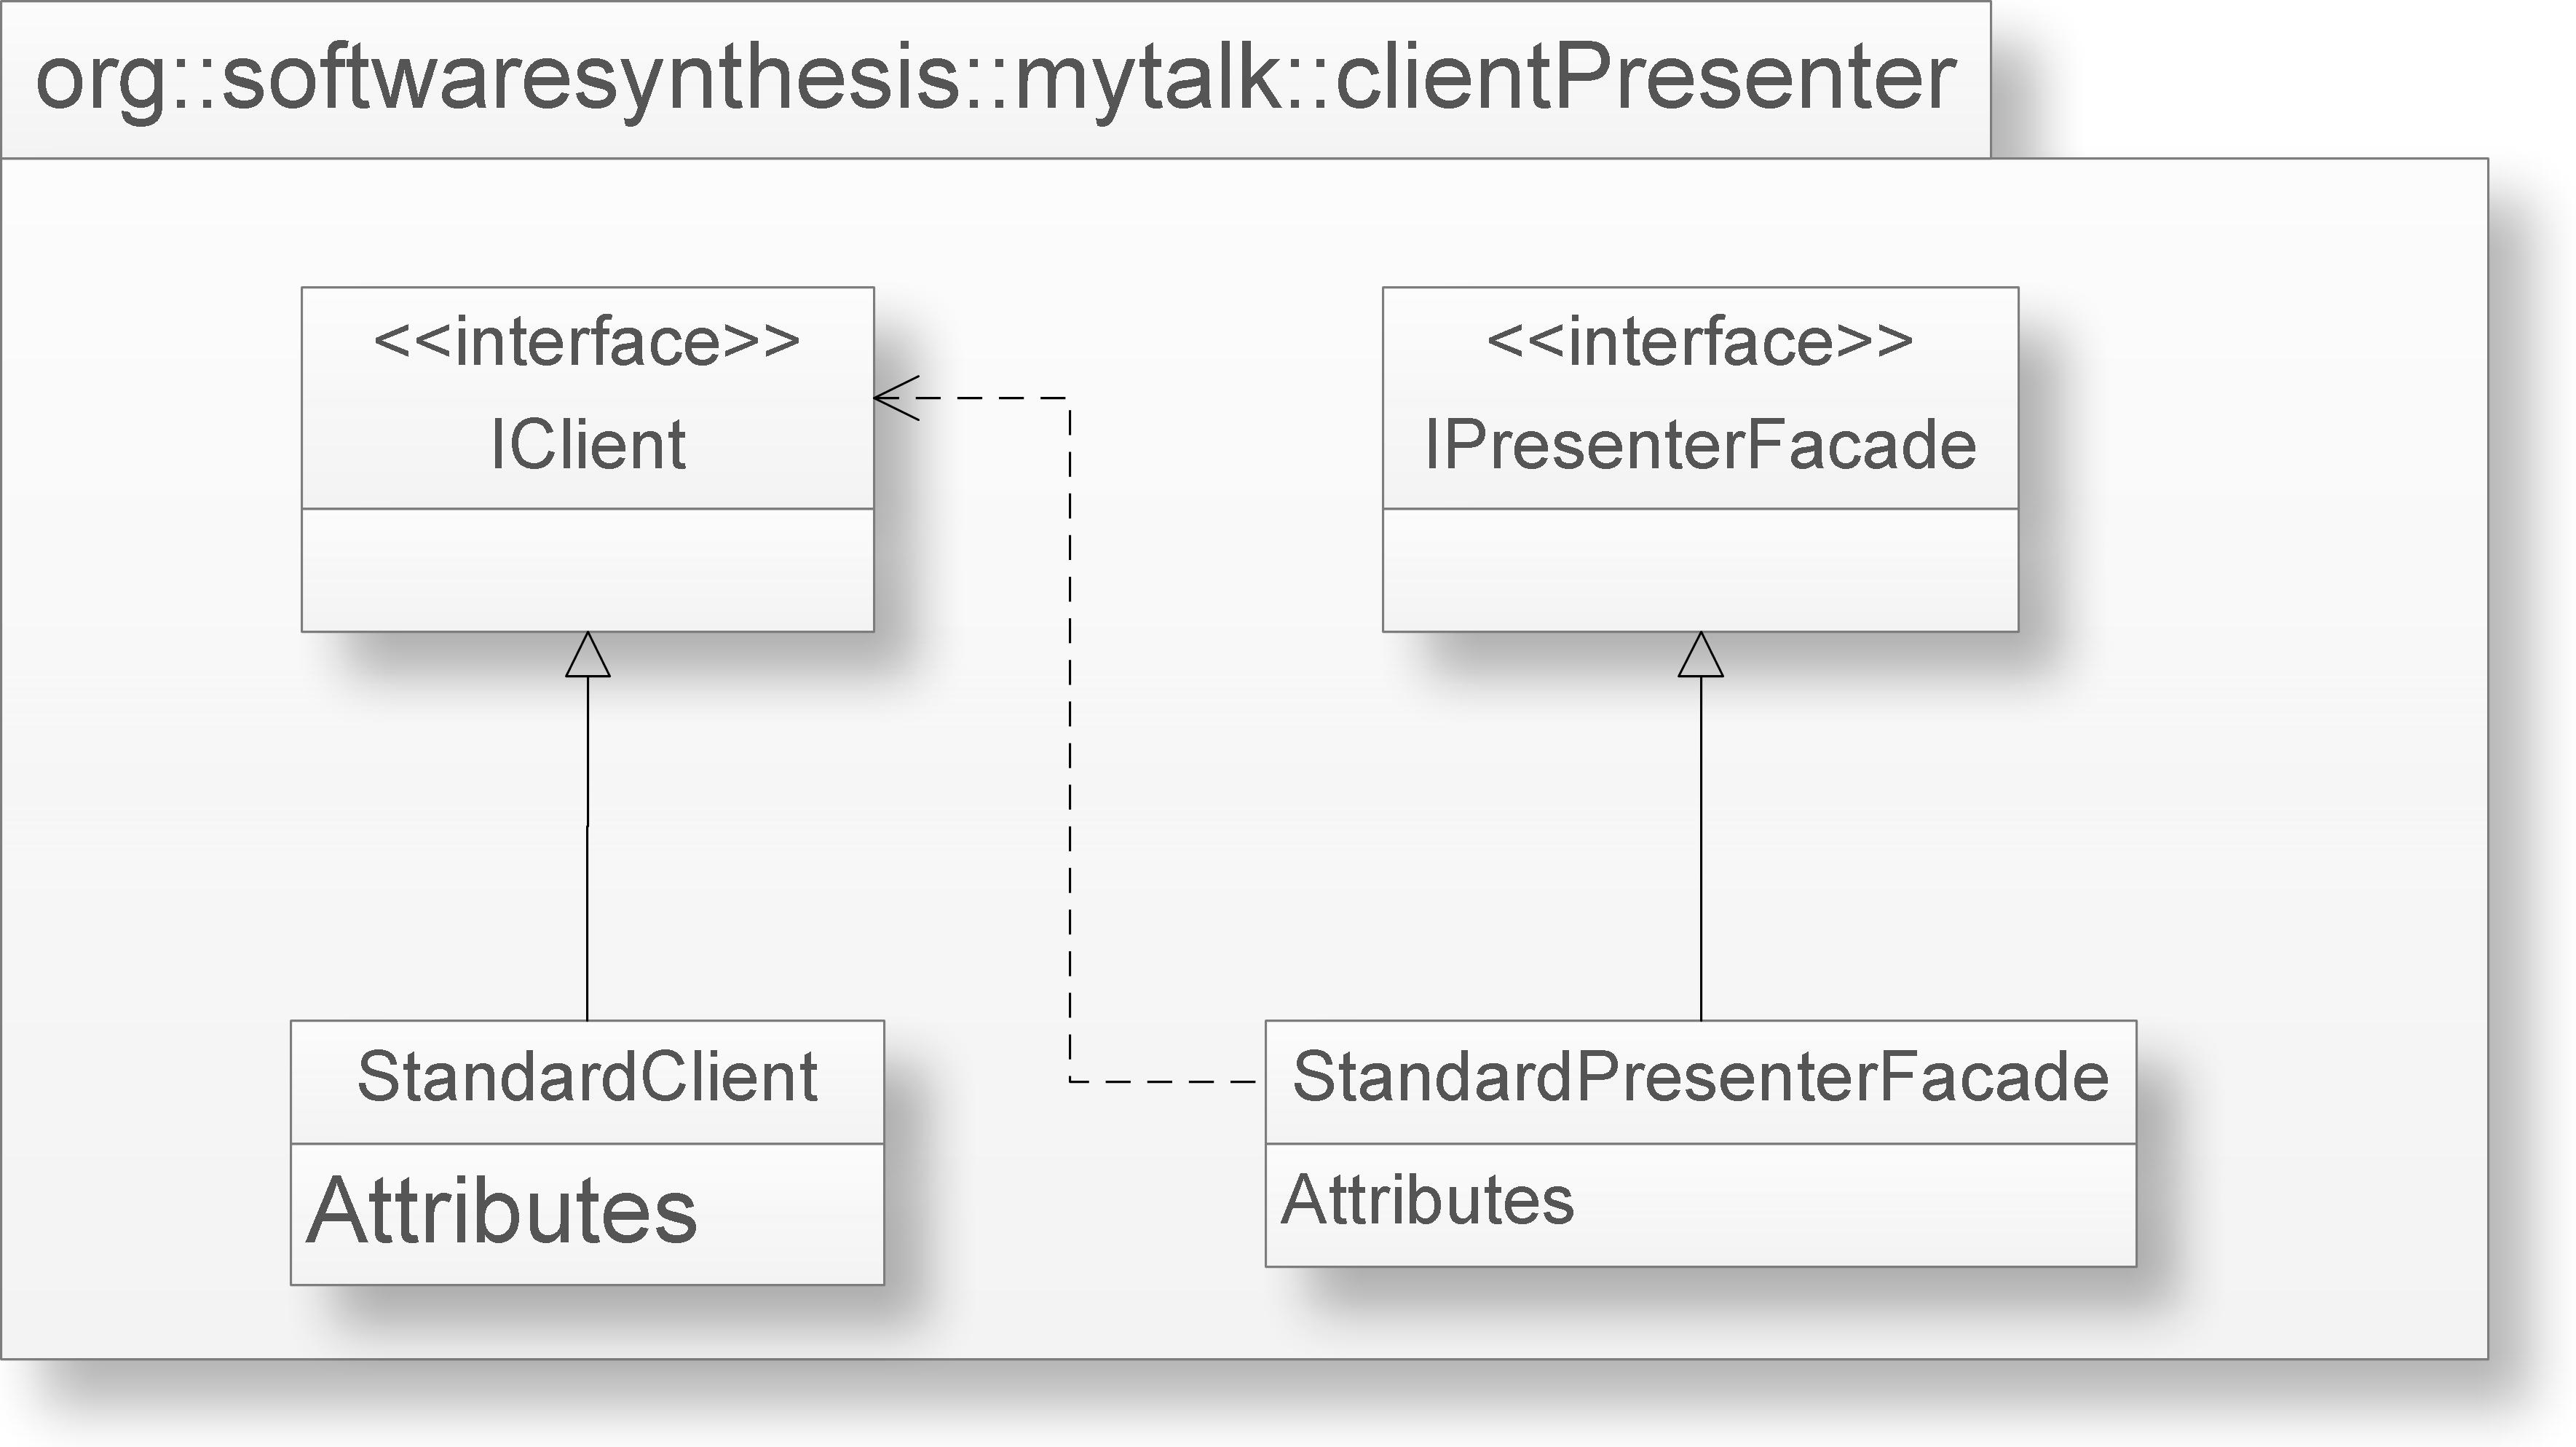
\includegraphics[width=.8\textwidth]{package_presenter}
\caption{Diagramma delle classi - Architettura mytalk.clientpresenter}\label{fig:package_presenter}
\end{center}
\end{figure}
\clearpage

\section{Architettura mytalk.clientview}
Come già accennato in precedenza, nella sezione introduttiva all'architettura e nella sezione del clientpresenter, clientview ha il compito di definire la logica di visualizzazione dei dati costituendo la GUI del sistema lato \underline{client}.

Le motivazioni che hanno portato a separare tale sotto-architettura dalla parte logica sono da ricercare nei vantaggi di riutilizzo del codice e semplificazione della manutenzione:
\begin{itemize}
 	\item \textbf{future espansioni}: innanzitutto tale scelta permetterà ai progettisti di sviluppare (in futuro) molteplici tipologie di ``viste'', implementabili liberamente svincolando i programmatori dal conoscere al dettaglio la logica sottostante per la gestione delle comunicazioni. Va comunque ricordato che in tal caso, gli sviluppatori dovranno avere un idea chiara del significato delle varie funzioni del Façade del presenter.
 	\item \textbf{semplificare la manutenzione}: cosi come scrivere da zero una nuova vista, anche modificare quelle già presenti risulta essere più facile, per gli stessi motivi descritti al punto precedente.
\end{itemize}

La sotto-architettura clientview rappresenta quindi una vista di default fornita dal team, con lo scopo di rappresentare in modo chiaro ed organizzato le possibilità di iterazione, da parte dell'utente finale, con l'applicativo \caName{}.

Nell'utilizzare tale vista l'utente non avrà la percezione di come sia stata progettata l'architettura totale del sistema, svincolandolo cosi dal dover conoscere le procedure necessarie all'esecuzione di una determinata operazione.

Per quanto riguarda la componentistica, la sotto-architettura clientview è dotata di:
\begin{itemize}[noitemsep,nolistsep]
	\item[-] Façade della vista
	\item[-] Gestione GUI
\end{itemize}

Per le specifiche dei componenti sopra citati, si rimanda alla sezione successiva.

Infine si fa notare che i nomi di tutte le classi riportate nella sezione sono implicitamente parte del package \texttt{org.softwaresynthesis.mytalk.clientview} pertanto tale prefisso sarà omesso nella loro denominazione.

\begin{figure}[h]
\centering
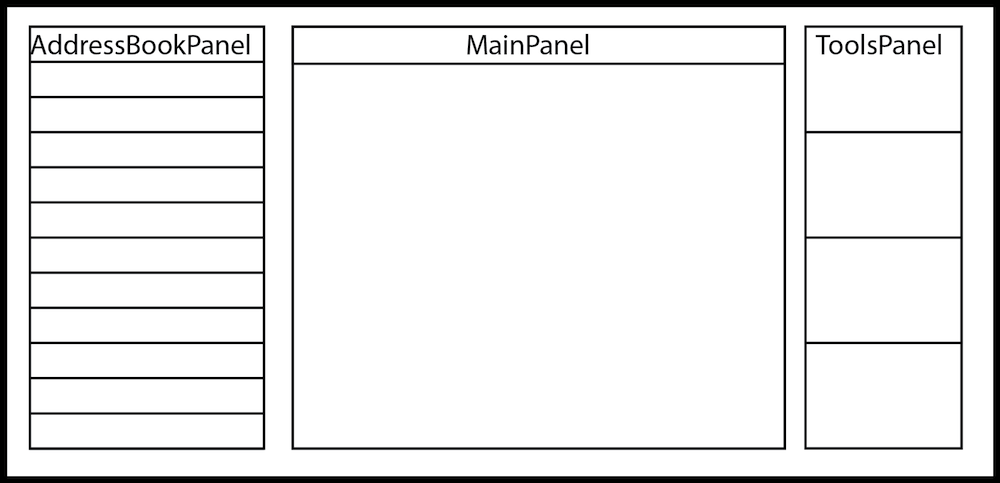
\includegraphics[width=\textwidth]{GUI}
\caption{Rappresentazione ad alto livello della GUI}\label{fig:gui}
\end{figure}

In figura \ref{fig:gui} si riporta un abbozzo dell'interfaccia grafica utente realizzata mediante le classi di questa sotto-architettura. In conformità con quanto stabilito dai requisiti (RSDO10.0.0) l'interfaccia si sviluppa in un'unica pagina.

In particolare, la parte denominata AddressBookPanel conterrà la lista degli utenti nella rubrica, mentre ToolsPanel conterrà i componenti grafici che rappresentano tutte le funzionalità offerte dal sistema. 

Il contenuto del MainPanel, invece, varia in relazione alla funzionalità scelta dall'utente in quel momento. Ad esempio, qualora l'utente selezioni un contatto presente nella rubrica, verrà visualizzato il profilo corrispondente al contatto scelto.

\subsection{Componenti evidenziati}

\subsubsection{Façade della vista}
\begin{description}
	\item{\scshape\bfseries Descrizione:}\\
Il compito di questo componente è rappresentare l'intera sotto-architettura clientview, per come viene vista dalle classi del presenter. In tal modo è possibile rendere indipendenti le classi concrete della sotto-architettura clientview in quanto le dipendenze funzionali provenienti dall'esterno sono accentrate nel Façade.

In particolare, tramite le operazioni che sono dichiarate nell'interfaccia \texttt{IViewFacade} si rende possibile l'aggiornamento dinamico a tempo di esecuzione della vista e, di conseguenza, di quello che viene visualizzato dall'utente finale del sistema.
	\item{\scshape\bfseries Diagramma delle classi:}
\begin{figure}[H]
\begin{center}
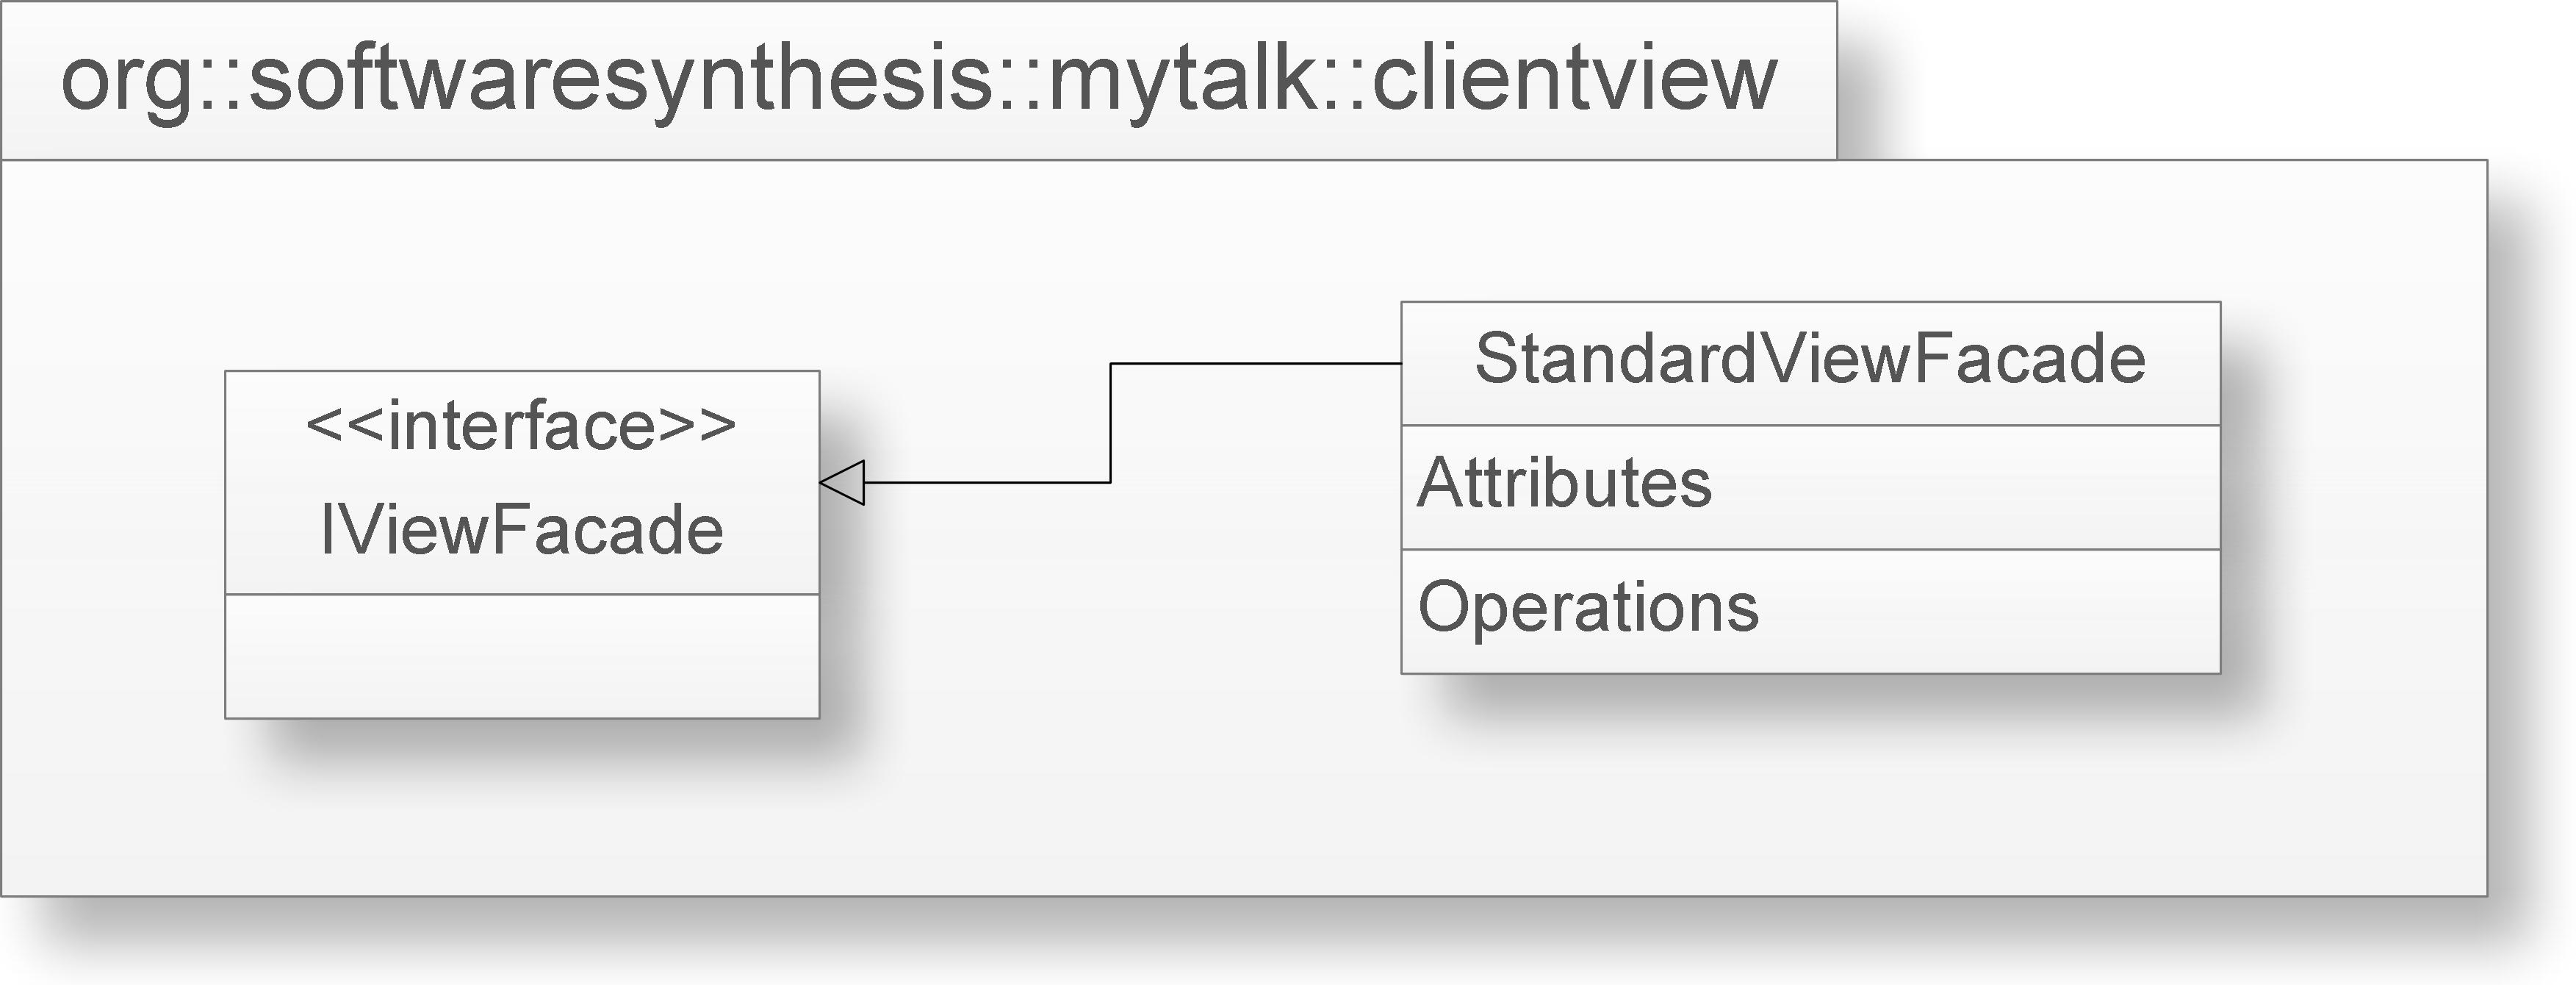
\includegraphics[width=.8\textwidth]{componenti_clientview}
\caption{Diagramma delle classi - Façade della vista}\label{fig:facade_vista}
\end{center}
\end{figure}
	\item{\scshape\bfseries Classi utilizzate:} 
	\begin{itemize}[noitemsep,nolistsep]
		\item[-] \texttt{IViewFacade}
		\item[-] \texttt{StandardViewFacade}
	\end{itemize}  
\end{description}

\subsubsection{Gestione GUI}
\begin{description}
	\item{\scshape\bfseries Descrizione:}\\
Questo componente si occupa della gestione dell'interfaccia grafica presentata all'utente finale. Le classi in esso contenute servono pertanto per la rappresentazione delle funzionalità offerte dal sistema all'utente.

Si noti che questo componente demanda tutta la logica al presenter, tramite il Façade del presenter, e quindi è relativo solo ed esclusivamente alla grafica. Inoltre l'interazione con esso è centralizzata all'interno della classe \texttt{gui.GUIHandler}, ciò significa che tutte le altre classi del package \texttt{gui} non interagiscono direttamente con il presenter.
	\item{\scshape\bfseries Diagramma delle classi:}
	
\begin{figure}[H]
\begin{center}
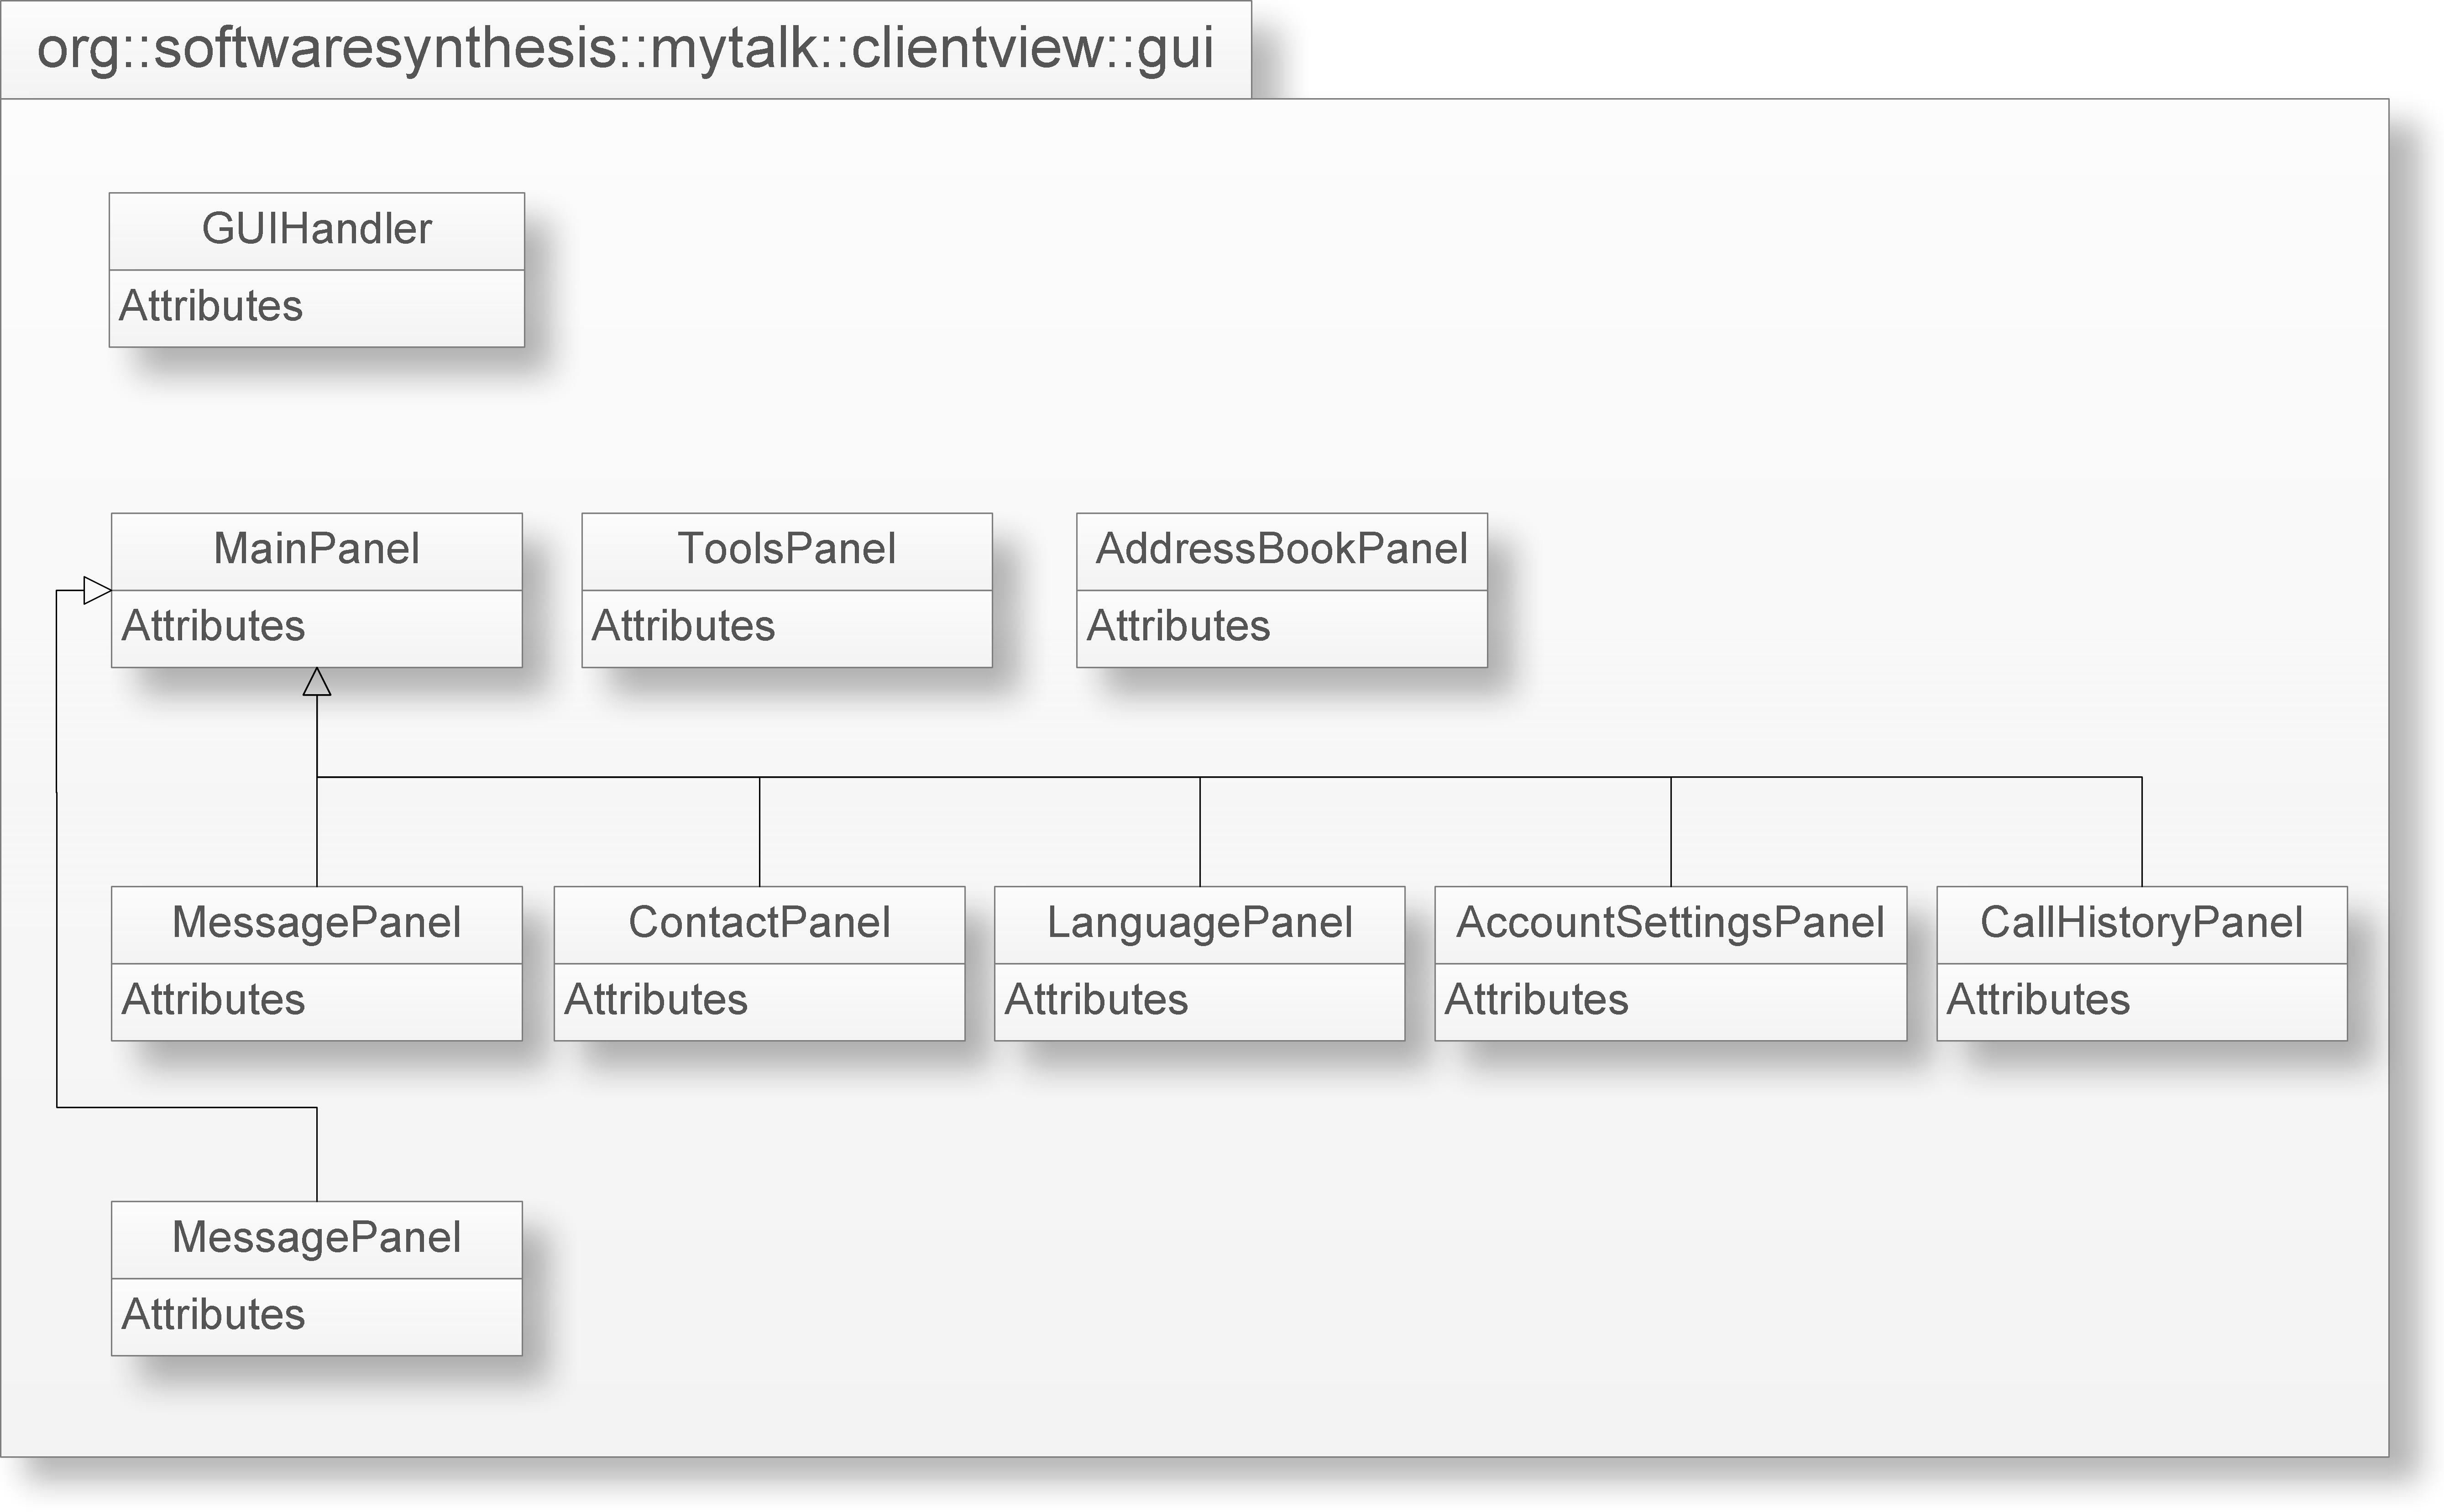
\includegraphics[width=.8\textwidth]{componenti_clientview_gui}
\caption{Diagramma delle classi - Gestione GUI}\label{fig:gestione_gui}
\end{center}
\end{figure}	
	
	\item{\scshape\bfseries Classi utilizzate:} 
	\begin{itemize}[noitemsep,nolistsep]
		\item[-] \texttt{gui.GUIHandler}
		\item[-] \texttt{gui.MainPanel}
		\item[-] \texttt{gui.ToolsPanel}
		\item[-] \texttt{gui.AddressBookPanel}
		\item[-] \texttt{gui.ContactPanel}
		\item[-] \texttt{gui.SearchResultPanel}
		\item[-] \texttt{gui.MessagePanel}
		\item[-] \texttt{gui.LanguagePanel}
		\item[-] \texttt{gui.AccountSettingsPanel}
		\item[-] \texttt{gui.CallHistoryPanel}
	\end{itemize}  
\end{description}

\subsection{Diagramma delle classi}
\begin{figure}[H]
\begin{center}
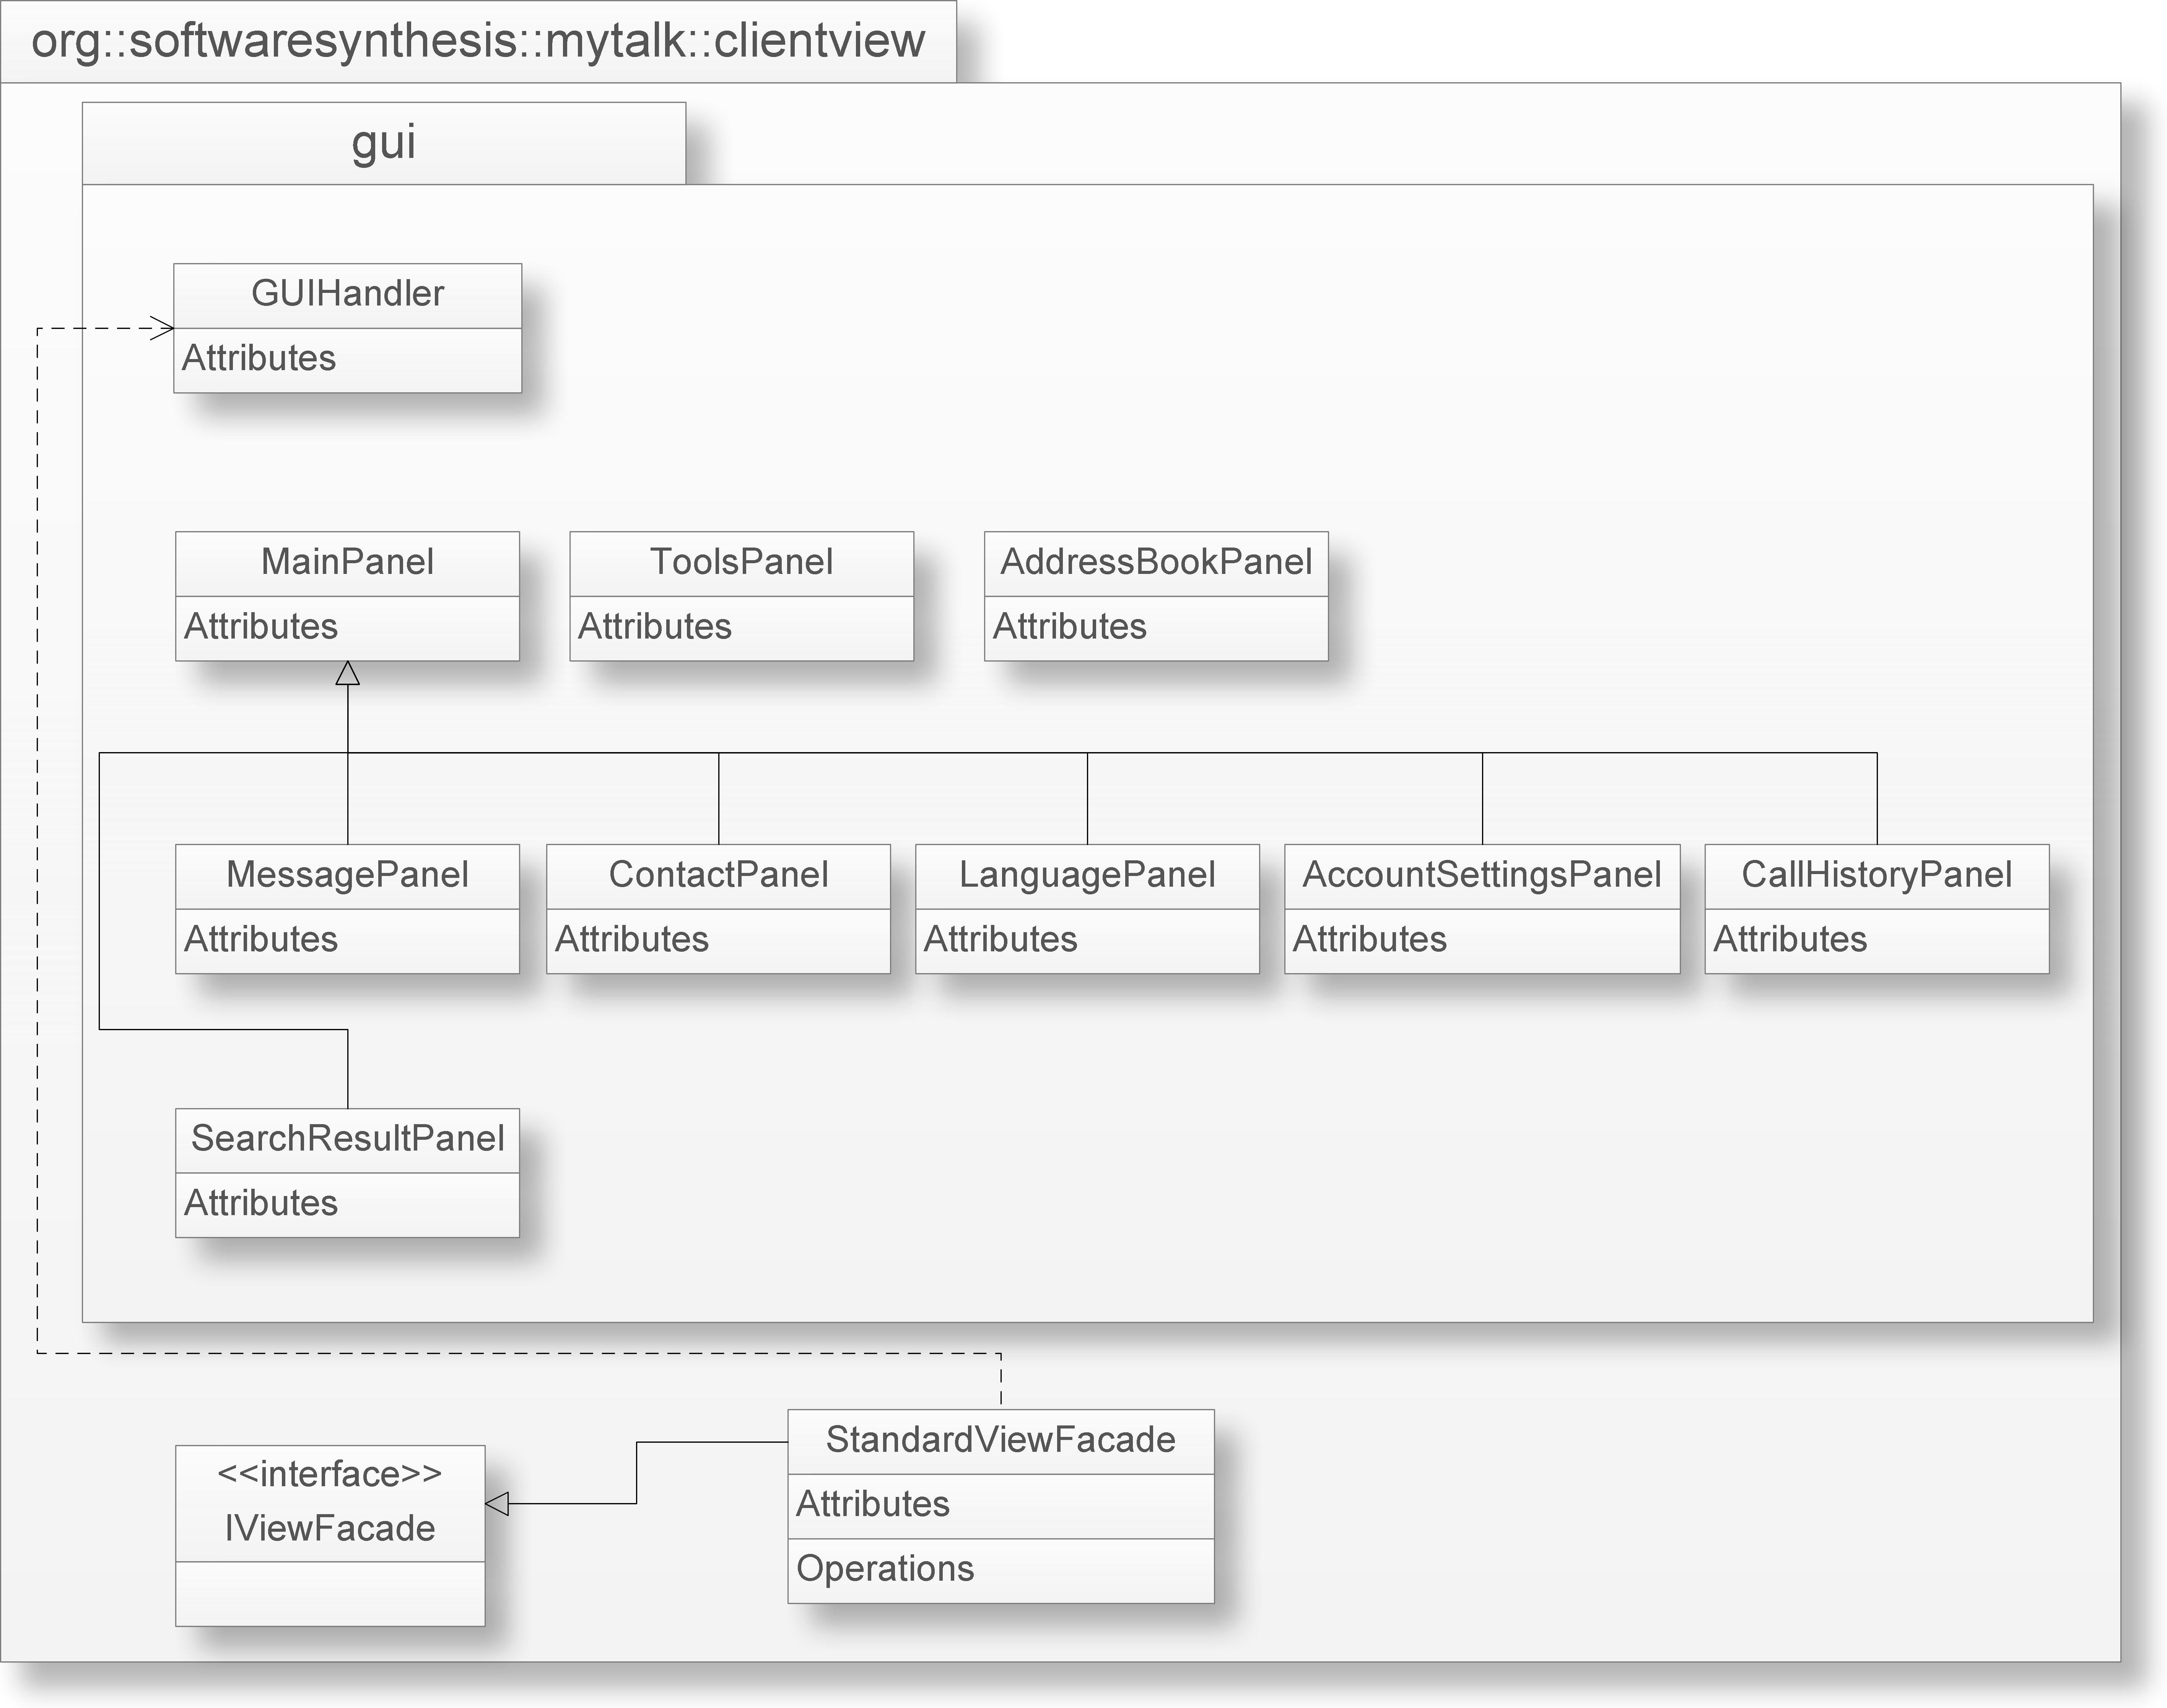
\includegraphics[width=1\textwidth]{Package_view}
\caption{Diagramma delle classi - Architettura mytalk.clientview}\label{fig:package_client_presenterview}
\end{center}
\end{figure}
\clearpage

\section{Descrizione delle classi}

\subsection{Package org.softwaresynthesis.mytalk.server.dao}

\subsubsection{IAudioMessage}
\begin{description}
	\item{\scshape\bfseries Descrizione:}\\
Interfaccia per i messaggi audio della segreteria telefonica che viene implementata dalle classi \texttt{AudioMessage} e dal relativo proxy \texttt{server.message.AudioMessageProxy}.
% contiene operazione astratta play() per riprodurre il messaggio (se presente) o scaricarlo e avviarne la riproduzione
	\item{\scshape\bfseries Componenti che ne fanno uso:}
	  \begin{itemize}[noitemsep,nolistsep]
	  \item[-] Gestione database
	  \item[-] Gestione segreteria
	  \end{itemize}
\end{description}

\subsubsection{IAudioVideoMessage}
\begin{description}
	\item{\scshape\bfseries Descrizione:}\\
Interfaccia per i messaggi audio/video della segreteria telefonica, a sua volta implementata dalle classi \texttt{AudioVideoMessage} e dal suo proxy \texttt{server.message.AudioVideoMessageProxy}.
% contiene operazione astratta play() per riprodurre il messaggio (se presente) o scaricarlo e avviarne la riproduzione
	\item{\scshape\bfseries Componenti che ne fanno uso:} 
	  \begin{itemize}[noitemsep,nolistsep]
	    \item[-] Gestione database
	    \item[-] Gestione segreteria
	  \end{itemize}
\end{description}

\subsubsection{AudioMessage}
\begin{description}
	\item{\scshape\bfseries Descrizione:}\\
Classe che rappresenta un messaggio audio nella segreteria telefonica di un utente, implementa l'interfaccia \texttt{IAudioMessage}.
	\item{\scshape\bfseries Componenti che ne fanno uso:}
	  \begin{itemize}[noitemsep,nolistsep]
	    \item[-] Gestione database
	    \item[-] Gestione segreteria
	  \end{itemize}
\end{description}

\subsubsection{AudioVideoMessage}
\begin{description}
	\item{\scshape\bfseries Descrizione:}\\
Classe che rappresenta un messaggio audio/video nella segreteria telefonica di un utente, implementa l'interfaccia \texttt{IAudioVideoMessage}.
	\item{\scshape\bfseries Componenti che ne fanno uso:}
	  \begin{itemize}[noitemsep,nolistsep]
	    \item[-] Gestione database
	    \item[-] Gestione segreteria
	  \end{itemize}
\end{description}

\subsubsection{IGroup}
\begin{description}
	\item{\scshape\bfseries Descrizione:}\\
Interfaccia per i gruppi interni alla rubrica, prevede un'operazione astratta \texttt{add(IUserData)} per l'aggiunta di un nuovo contatto al gruppo e un'operazione \texttt{remove(IUserData)} per la sua rimozione.

Estende inoltre l'interfaccia \texttt{server.abook.IContact} comune a tutti i contatti della rubrica e richiesta per l'applicazione del \underline{design pattern} Composite.
	\item{\scshape\bfseries Componenti che ne fanno uso:} 
	  \begin{itemize}[noitemsep,nolistsep]
	    \item[-] Gestione database
	    \item[-] Gestione rubrica
	  \end{itemize}
\end{description}

\subsubsection{StandardGroup}
\begin{description}
	\item{\scshape\bfseries Descrizione:}\\
Implementazione dell'interfaccia \texttt{IGroup}, ogni gruppo è dotato di un nome e raccoglie in sé zero o più istanze di classi sottotipo di \texttt{server.abook.IContact}.
	\item{\scshape\bfseries Componenti che ne fanno uso:}
	  \begin{itemize}[noitemsep,nolistsep]
	    \item[-] Gestione database
	  \end{itemize}
\end{description}

\subsubsection{IUserData}
\begin{description}
	\item{\scshape\bfseries Descrizione:}\\
Interfaccia per le classi che rappresentano gli utenti, è dotata di operazioni get/set per accedere ai dati degli utenti registrati sul sistema.
	\item{\scshape\bfseries Componenti che ne fanno uso:}
	\begin{itemize}[noitemsep,nolistsep]
	  \item[-] Gestione database
	  \item[-] Gestione rubrica
	  \item[-] Gestione connessione
	\end{itemize}
\end{description}

\subsubsection{StandardUserData}
\begin{description}
	\item{\scshape\bfseries Descrizione:}\\
Classe che implementa l'interfaccia \texttt{IUserData} le cui istanze corrispondono ai record della tabella degli utenti nel \underline{database}.
	\item{\scshape\bfseries Componenti che ne fanno uso:}
	\begin{itemize}[noitemsep,nolistsep]
	  \item[-] Gestione database
	  \item[-] Gestione stato
	\end{itemize}
\end{description}

\subsection{Package org.softwaresynthesis.mytalk.server.connection}

\subsubsection{ICommunicationHandler}
\begin{description}
	\item{\scshape\bfseries Descrizione:}\\
Interfaccia per la gestione delle richieste per ottenere le informazioni necessarie a un \underline{client} per stabilire una comunicazione con altri \underline{client}. In particolare le operazioni in essa dichiarate dovranno ritornare un istanza di un oggetto che implementa \texttt{IConnection}.
	\item{\scshape\bfseries Componenti che ne fanno uso:}
		\begin{itemize}[noitemsep,nolistsep]
			\item[-] Gestione connessione
		\end{itemize}
\end{description}

\subsubsection{StandardCommunicationHandler}
\begin{description}
	\item{\scshape\bfseries Descrizione:}\\
Implementazione che si fornisce dell'interfaccia \texttt{ICommunicationHandler}. In tale classe, le informazioni ritornate al \underline{client} sono informazioni necessarie a stabilire una connessione di tipo WebRTC (ritorna un istanza di \texttt{WebRTCInfo}).
	\item{\scshape\bfseries Componenti che ne fanno uso:}
		\begin{itemize}[noitemsep,nolistsep]
			\item[-] Gestione connessione
		\end{itemize}
\end{description}

\subsubsection{IConnection}
\begin{description}
	\item{\scshape\bfseries Descrizione:}\\
Interfaccia mediante la quale è possibile recuperare  i dati necessari a un \underline{client} al fine di stabilire una connessione con un altro \underline{client}.
	\item{\scshape\bfseries Componenti che ne fanno uso:}
		\begin{itemize}[noitemsep,nolistsep]
			\item[-] Gestione connessione
			\item[-] Gestione comunicazione
		\end{itemize}
\end{description}

\subsubsection{WebRTCInfo}
\begin{description}
	\item{\scshape\bfseries Descrizione:}\\
Implementazione dell'interfaccia \texttt{IConnection} che rappresenta le informazioni usate da un \underline{client} per stabilire una connessione WebRTC con un altro \underline{client}.
	\item{\scshape\bfseries Componenti che ne fanno uso:}
		\begin{itemize}[noitemsep,nolistsep]
			\item[-] Gestione connessione
		\end{itemize}
\end{description}

\subsection{Package org.softwaresynthesis.mytalk.server.abook}

\subsubsection{IContact}
\begin{description}
	\item{\scshape\bfseries Descrizione:}\\
Interfaccia condivisa da tutti i contatti della rubrica di un utente, permette di trattare in modo uniforme gli utenti singoli e i gruppi secondo quando previsto dal \underline{design pattern} Composite.

Dichiara la presenza di operazioni astratte per recuperare l'accesso alle informazioni sottostanti (ad esempio il nome di un utente o di un gruppo).
	\item{\scshape\bfseries Componenti che ne fanno uso:}
	\begin{itemize}[nolistsep, noitemsep]
	  \item[-] Gestione rubrica
	\end{itemize}
\end{description}

\subsubsection{IAddressBook}
\begin{description}
	\item{\scshape\bfseries Descrizione:}\\
Interfaccia che raccoglie le operazioni sulla rubrica e permette di controllare l'accesso alle strutture dati che la implementano.
	\item{\scshape\bfseries Componenti che ne fanno uso:}
	\begin{itemize}[noitemsep,nolistsep]
	  \item[-] Gestione rubrica
	\end{itemize}
\end{description}

\subsubsection{UserDataProxy}
\begin{description}
  \item{\scshape\bfseries Descrizione:}\\
La classe implementa l'interfaccia \texttt{server.dao.IUserData} e rappresenta un proxy per i dati degli utenti che risiedono sul \underline{server}.

Le istanze di questa classe vengono restituite da un opportuno Factory Method dichiarato nell'interfaccia \texttt{server.ServerFacade} e hanno il ruolo di rappresentare sui \underline{client} degli oggetti che risiedono in un diverso spazio di indirizzamento (sul \underline{server}) nonché di controllare gli accessi per esigenze di protezione.
  \item{\scshape\bfseries Componenti che ne fanno uso:}
  \begin{itemize}[noitemsep,nolistsep]
    \item[-] Gestione rubrica
  \end{itemize}
\end{description}

\subsubsection{AddressBook}
\begin{description}
	\item{\scshape\bfseries Descrizione:}\\
Classe che implementa l'interfaccia \texttt{IAddressBook} e rappresenta quindi la rubrica di un determinato utente. Contiene un riferimento a \texttt{IContact} che corrisponde al nodo padre della struttura dati ad albero contenente la rubrica.
	\item{\scshape\bfseries Componenti che ne fanno uso:}
	\begin{itemize}[noitemsep,nolistsep]
	  \item[-] Gestione rubrica
	\end{itemize}
\end{description}

\subsection{Package org.softwaresynthesis.mytalk.server.state}
\subsubsection{IState}
\begin{description}
	\item{\scshape\bfseries Descrizione:}\\
Interfaccia padre della gerarchia di stati che gli utenti possono assumere nel corso dell'interazione con il sistema. La composizione delle istanze di \texttt{server.dao.StandardUserData} con oggetti sottotipo di \texttt{IState} cui inoltrano le richieste ricevute dall'esterno permette di cambiare dinamicamente il comportamento degli oggetti che rappresentano gli utenti.
	\item{\scshape\bfseries Componenti che ne fanno uso:}
	\begin{itemize}[noitemsep,nolistsep]
	  \item[-] Gestione stato
	  \item[-] Gestione connessione
	\end{itemize}
\end{description}

\subsubsection{StateOnline}
\begin{description}
	\item{\scshape\bfseries Descrizione:}\\
Classe astratta che implementa l'interfaccia \texttt{IState} e viene estesa da tutti gli stati che corrispondono alla presenza ``online'' dell'utente. È ulteriormente specializzata dalle sottoclassi concrete \texttt{StateAvailable} e \texttt{StateOccupied}, le quali hanno facoltà di determinare il reale comportamento degli utenti online.
	\item{\scshape\bfseries Componenti che ne fanno uso:}
	\begin{itemize}[noitemsep,nolistsep]
	  \item[-] Gestione stato
	\end{itemize}
\end{description}

\subsubsection{StateOffline}
\begin{description}
	\item{\scshape\bfseries Descrizione:}\\
Classe concreta della gerarchia degli stati che implementa l'interfaccia \texttt{IState} e corrisponde alla mancata presenza online dell'utente che la possiede. Un utente che si trova nello stato ``offline'' non può essere contattato direttamente ma solo attraverso la segreteria telefonica.
	\item{\scshape\bfseries Componenti che ne fanno uso:}
	\begin{itemize}[noitemsep,nolistsep]
	  \item[-] Gestione stato
	\end{itemize}
\end{description}

\subsubsection{StateAvailable}
\begin{description}
	\item{\scshape\bfseries Descrizione:}\\
Classe concreta della gerarchia degli stati che corrisponde alla presenza online di un utente e alla sua disponibilità ad accettare comunicazioni in ingresso.
	\item{\scshape\bfseries Componenti che ne fanno uso:}
    \begin{itemize}[noitemsep,nolistsep]
      \item[-] Gestione stato
    \end{itemize}
\end{description}

\subsubsection{StateOccupied}
\begin{description}
	\item{\scshape\bfseries Descrizione:}\\
Classe concreta della gerarchia degli stati che corrisponde alla mancata disponibilità di un utente a ricevere ulteriori comunicazioni in ingresso dal momento che si trova impegnato in un'altra conversazione. Gli utenti che si trovano in questo stato non possono essere contattati direttamente ma solo attraverso la possibilità di lasciare un messaggio in segreteria.
	\item{\scshape\bfseries Componenti che ne fanno uso:}
	\begin{itemize}[noitemsep,nolistsep]
	  \item[-] Gestione stato
	\end{itemize}
\end{description}

\subsection{Package org.softwaresynthesis.mytalk.server.message}
\subsubsection{IMessageBox}
\begin{description}
	\item{\scshape\bfseries Descrizione:}\\
Interfaccia che rappresenta, ad alto livello, la segreteria telefonica dell'utente cui è associata. Tramite opportune operazioni permette di accedere all'elenco dei messaggi audio o audio/video che l'utente ha ricevuto nel periodo in cui era in linea o non era disponibile perché impegnato in una conversazione.
	\item{\scshape\bfseries Componenti che ne fanno uso:}
	\begin{itemize}
	  \item[-] Gestione segreteria
	\end{itemize}
\end{description}

\subsubsection{StandardMessageBox}
\begin{description}
	\item{\scshape\bfseries Descrizione:}\\
Classe concreta che implementa l'interfaccia \texttt{IMessageBox} e rappresenta dunque la rubrica associata a un determinato utente.
	\item{\scshape\bfseries Componenti che ne fanno uso:}
	\begin{itemize}[noitemsep,nolistsep]
	  \item[-] Gestione segreteria
	\end{itemize}
\end{description}

\subsubsection{AudioMessageProxy}
\begin{description}
	\item{\scshape\bfseries Descrizione:}\\
Proxy virtuale ad uso dei \underline{client} per i messaggi audio lasciati ad un utente in segreteria. La classe implementa l'interfaccia \texttt{server.dao.IAudioMessage} ogni sua istanza è costruita per composizione con un riferimento a  \texttt{server.dao.AudioMessage}, cui inoltra le richieste dopo aver eventualmente scaricato il messaggio dal \underline{server}.
	\item{\scshape\bfseries Componenti che ne fanno uso:}
	\begin{itemize}[noitemsep,nolistsep]
	  \item[-] Gestione segreteria
	\end{itemize}
\end{description}

\subsubsection{AudioVideoMessageProxy}
\begin{description}
	\item{\scshape\bfseries Descrizione:}\\
Proxy virtuale ad uso dei \underline{client} per i messaggi audio/video in segreteria. La classe implementa l'interfaccia \texttt{server.dao.AudioVideoMessage} ed è costruita, similmente a \texttt{AudioMessageProxy} con un'istanza di \texttt{server.dao.AudioVideoMessage} per limitare il traffico di rete e ottimizzare il consumo di memoria del \underline{client}.
	\item{\scshape\bfseries Componenti che ne fanno uso:}
	\begin{itemize}[noitemsep,nolistsep]
	  \item[-] Gestione segreteria
	\end{itemize}
\end{description}

\subsection{Package org.softwaresynthesis.mytalk.server}
\subsubsection{IServerFacade}
\begin{description}
	\item{\scshape\bfseries Descrizione:}\\
Interfaccia che contiene tutte le operazioni richieste dai componenti della sotto-architettura clientpresenter inerenti alla registrazione, all'autenticazione,  alla gestione della rubrica e della segreteria nonché delle connessioni con altri utenti.

In quest'ultimo caso le operazioni richieste vengono a loro volta inoltrate al componente responsabile della gestione della connessione (\texttt{server.connection.IConnectionHandler}).
	\item{\scshape\bfseries Componenti che ne fanno uso:}
	\begin{itemize}[noitemsep,nolistsep]
	  \item[-] Façade del server
	  \item[-] Façade del presenter
	  \item[-] Gestione comunicazione
	\end{itemize}
\end{description}

\subsubsection{StandardServerFacade}
\begin{description}
	\item{\scshape\bfseries Descrizione:}\\
Questa classe Singleton è l'implementazione dell'interfaccia \texttt{IServerFacade} e contiene, in particolare, i metodi che rendono concrete le operazioni corrispondenti ai Factory Method dichiarati nell'interfaccia citata (per la gestione dei messaggi in segreteria e degli utenti nella rubrica).
	\item{\scshape\bfseries Componenti che ne fanno uso:}
	\begin{itemize}[noitemsep,nolistsep]
	  \item[-] Façade del server
	\end{itemize}
\end{description}

\subsection{Package org.softwaresynthesis.mytalk.clientpresenter}
\subsubsection{IClient}
\begin{description}
	\item{\scshape\bfseries Descrizione:}\\
Interfaccia che raccoglie le operazioni astratte che è possibile invocare su un \underline{client} astratto del sistema corrispondenti, ad esempio, alla ricezione di una chiamata in ingresso oppure all'interrogazione sullo stato (nodo semplice o Supernodo) di un determinato \underline{client}.
	\item{\scshape\bfseries Componenti che ne fanno uso:}
	\begin{itemize}[noitemsep,nolistsep]
	  \item[-] Gestione comunicazione
	\end{itemize}
\end{description}

\subsubsection{StandardClient}
\begin{description}
	\item{\scshape\bfseries Descrizione:}\\
Implementazione dell'interfaccia \texttt{IClient} che incapsula al suo interno la logica di eventuale ritrasmissione dei dati in ingresso (nel caso in cui il \underline{client} sia un Supernodo) e di invio dei dati prodotti in locale ai \underline{client} con cui è stata instaurata una connessione. 
	\item{\scshape\bfseries Componenti che ne fanno uso:}
	\begin{itemize}[noitemsep,nolistsep]
	  \item[-] Gestione comunicazione
	\end{itemize}
\end{description}

\subsubsection{IPresenterFacade}
\begin{description}
	\item{\scshape\bfseries Descrizione:}\\
Interfaccia che raccoglie la dichiarazione di tutte le operazioni astratte con cui si suppone che la vista realizzi lo scambio di messaggi con il presenter. Tramite queste operazioni deve dunque essere possibile, ad esempio, gestire l'autenticazione di un utente, interrogare la segreteria telefonica, modificare lo stato e le informazioni personali e scaricare la rubrica.
	\item{\scshape\bfseries Componenti che ne fanno uso:}
	\begin{itemize}[noitemsep,nolistsep]
	  \item[-] Façade del presenter
	  \item[-] Gestione GUI
	\end{itemize}
\end{description}

\subsubsection{StandardPresenterFacade}
\begin{description}
	\item{\scshape\bfseries Descrizione:}\\
Questa classe rappresenta un'applicazione del \underline{design pattern} Singleton e implementa inoltre l'interfaccia \texttt{IPresenterFacade}. Fornisce pertanto dei metodi concreti utilizzati per la comunicazione fra la vista e il \underline{server}, elaborando qualora necessario i dati ricevuti in input e inoltrando le richieste al componente Façade del server.
	\item{\scshape\bfseries Componenti che ne fanno uso:}
	\begin{itemize}[noitemsep,nolistsep]
	  \item[-] Façade del presenter
	\end{itemize}
\end{description}

\subsection{Package org.softwaresynthesis.mytalk.clientview}
\subsubsection{IViewFacade}
\begin{description}
  \item{\scshape\bfseries Descrizione}\\
Interfaccia che dichiara le operazioni astratte che possono essere richiamate sulla vista a partire dai componenti della sotto-architettura clientpresenter.
  \item{\scshape\bfseries Componenti che ne fanno uso:}
  \begin{itemize}[noitemsep,nolistsep]
    \item[-] Façade della vista
    \item[-] Façade del presenter
  \end{itemize}
\end{description}

\subsubsection{StandardViewFacade}
\begin{description}
  \item{\scshape\bfseries Descrizione}\\
Implementazione dell'interfaccia \texttt{IViewFacade} che contiene la definizione concreta dei metodi in essa dichiarati.
  \item{\scshape\bfseries Componenti che ne fanno uso:}
  \begin{itemize}[noitemsep,nolistsep]
    \item[-] Façade della vista
  \end{itemize}
\end{description}

\subsection{Package org.softwaresynthesis.clientview.gui}
\subsubsection{GUIHandler}
\begin{description}
  \item{\scshape\bfseries Descrizione}\\
L'istanza di questa classe ha il compito di inoltrare ai componenti delle diverse sotto-architetture le richieste provenienti dalle altre classi di questo package, in quanto unico possessore di un riferimento di tipo \texttt{IServerFacade}.

Inoltre, tale classe ha la responsabilità di controllare l'attivazione e gli aggiornamenti dinamici nel corso dell'esecuzione di tutti gli oggetti di classi grafiche istanziate.
  \item{\scshape\bfseries Componenti che ne fanno uso:}
  \begin{itemize}[noitemsep,nolistsep]
    \item[-] Gestione GUI
  \end{itemize}
\end{description}

\subsubsection{AddressBookPanel}
\begin{description}
  \item{\scshape\bfseries Descrizione}\\
Pannello che permette la visualizzazione della rubrica dell'utente connesso al sistema, e di accedere alle funzionalità di amministrazione della rubrica stessa (come l'aggiunta o la rimozione di utenti/gruppi, lo spostamento di un utente da un gruppo a un altro oppure l'ordinamento).
  \item{\scshape\bfseries Componenti che ne fanno uso:}
  \begin{itemize}[noitemsep,nolistsep]
    \item[-] Gestione GUI
  \end{itemize}
\end{description}

\subsubsection{MainPanel}
\begin{description}
  \item{\scshape\bfseries Descrizione}\\
Classe padre della gerarchia di oggetti grafici che possono comparire nella sezione principale dell'interfaccia utente. La parte comune a tutte le sottoclassi permette all'utente di impostare il proprio stato e di uscire dall'applicazione. Ogni sua specializzazione si rivolge a \texttt{GUIHandler} per inoltrare i comandi verso il componente Façade del presenter.
  \item{\scshape\bfseries Componenti che ne fanno uso:}
  \begin{itemize}[noitemsep,nolistsep]
    \item[-] Gestione GUI
  \end{itemize}
\end{description}

\subsubsection{ToolsPanel}
\begin{description}
  \item{\scshape\bfseries Descrizione}\\
Classe che rappresenta il pannello degli strumenti della home screen dell'applicativo, mediante il quale è possibile accedere alle funzionalità di ricerca, di segreteria telefonica, selezione della lingua, modifica dei dati dell'utente e storico delle chiamate.
  \item{\scshape\bfseries Componenti che ne fanno uso:}
  \begin{itemize}[noitemsep,nolistsep]
    \item[-] Gestione GUI
  \end{itemize}
\end{description}

\subsubsection{SearchResultPanel}
\begin{description}
  \item{\scshape\bfseries Descrizione}\\
Componente grafica che estende la classe \texttt{MainPanel} e visualizza i risultati della ricerca di un utente. La sua visualizzazione avviene in seguito all'uso della componente grafica di ricerca presente nel pannello degli strumenti.
  \begin{itemize}[noitemsep,nolistsep]
    \item[-] Gestione GUI
  \end{itemize}
\end{description}

\subsubsection{ContactPanel}
\begin{description}
  \item{\scshape\bfseries Descrizione}\\
Sottoclasse di \texttt{MainPanel} utilizzata per rappresentare il profilo di un utente. Solo accedendo quest'ultimo sarà possibile avviare una comunicazione con l'utente. Il contatto viene visualizzato selezionando l'utente dalla rubrica oppure tra i risultati di una ricerca.
  \item{\scshape\bfseries Componenti che ne fanno uso:}
  \begin{itemize}[noitemsep,nolistsep]
    \item[-] Gestione GUI
  \end{itemize}
\end{description}

\subsubsection{MessagePanel}
\begin{description}
  \item{\scshape\bfseries Descrizione}\\
Questa sottoclasse di \texttt{MainPanel} permette di accedere all'elenco dei messaggi in segreteria di un determinato utente e ne permette la gestione. La visualizzazione si attiva quando viene premuto il relativo pulsante mostrato dall'istanza di \texttt{ToolsPanel}.
  \item{\scshape\bfseries Componenti che ne fanno uso:}
  \begin{itemize}[noitemsep,nolistsep]
    \item[-] Gestione GUI
  \end{itemize}
\end{description}

\subsubsection{LanguagePanel}
\begin{description}
  \item{\scshape\bfseries Descrizione}\\
Questa sottoclasse di \texttt{MainPanel} è impiegata per permettere da parte dell'utente finale la selezione della lingua desiderata. La visualizzazione del pannello avviene in seguito all'attivazione del pulsante corrispondente situato nel pannello degli strumenti.
  \item{\scshape\bfseries Componenti che ne fanno uso:}
  \begin{itemize}[noitemsep,nolistsep]
    \item[-] Gestione GUI
  \end{itemize}
\end{description}

\subsubsection{AccountSettingsPanel}
\begin{description}
  \item{\scshape\bfseries Descrizione}\\
Questa classe è utilizzata per rappresentare il \underline{form} che si presenta all'utente per la modifica dei propri dati. Costituisce inoltre una sottoclasse di \texttt{MainPanel} e viene visualizzata quando l'utente preme il relativo pulsante nel pannello degli strumenti.
  \item{\scshape\bfseries Componenti che ne fanno uso:}
  \begin{itemize}[noitemsep,nolistsep]
    \item[-] Gestione GUI
  \end{itemize}
\end{description}

\subsubsection{CallHistoryPanel}
\begin{description}
  \item{\scshape\bfseries Descrizione}\\
Questa classe estende \texttt{MainPanel} e viene impiegata per rappresentare lo storico delle chiamate visualizzato quando l'utente attiva il pulsante corrispondente presente nel \texttt{ToolsPanel}.
  \item{\scshape\bfseries Componenti che ne fanno uso:}
  \begin{itemize}[noitemsep,nolistsep]
    \item[-] Gestione GUI
  \end{itemize}
\end{description}
\clearpage

\section{Conclusioni sull'architettura}

\subsection{Diagrammi delle attività}
In questa sezione saranno descritti i diagrammi di attività che rappresentano il flusso di utilizzo dei vari servizi messi a disposizione dal prodotto \caName.

\begin{figure}[H]
\centering
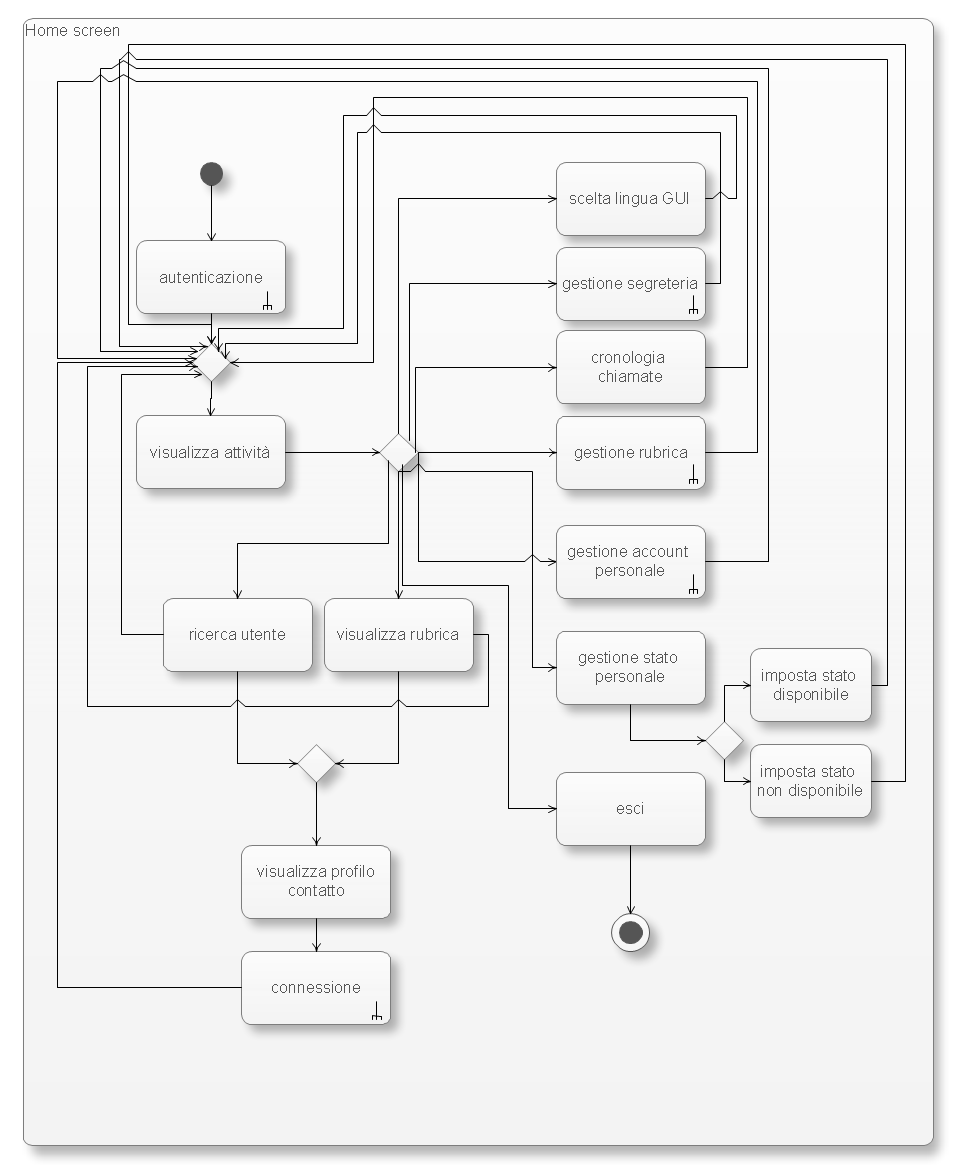
\includegraphics[width=.8\textwidth]{home}
\caption{Diagramma di attività generale che descrive l'interazione con il sistema}\label{fig:ADhome}
\end{figure}

Il diagramma in figura \vref{fig:ADhome} rappresenta il flusso principale dell'applicazione \caName. Da tale punto è possibile autenticarsi al sistema per poi poter usufruire di tutti i servizi messi a disposizione dal prodotto. Nei successivi diagrammi, figura \ref{fig:ADregistrazione} e \ref{fig:ADrecuperopassword}, vengono descritti rispettivamente le specializzazioni delle attività presenti nella schermata di login: registrazione (se non si ha ancora a disposizione un account utente) e recupero password (nel caso la password sia stata smarrita).

\begin{figure}[H]
\centering
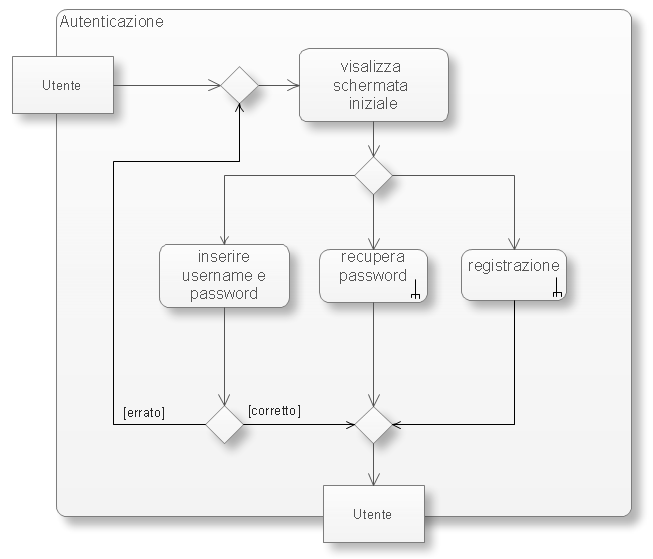
\includegraphics[width=.8\textwidth]{autenticazione}
\caption{Diagramma di attività relativo all'autententicazione}\label{fig:ADautenticazione}
\end{figure}

\begin{figure}[H]
\centering
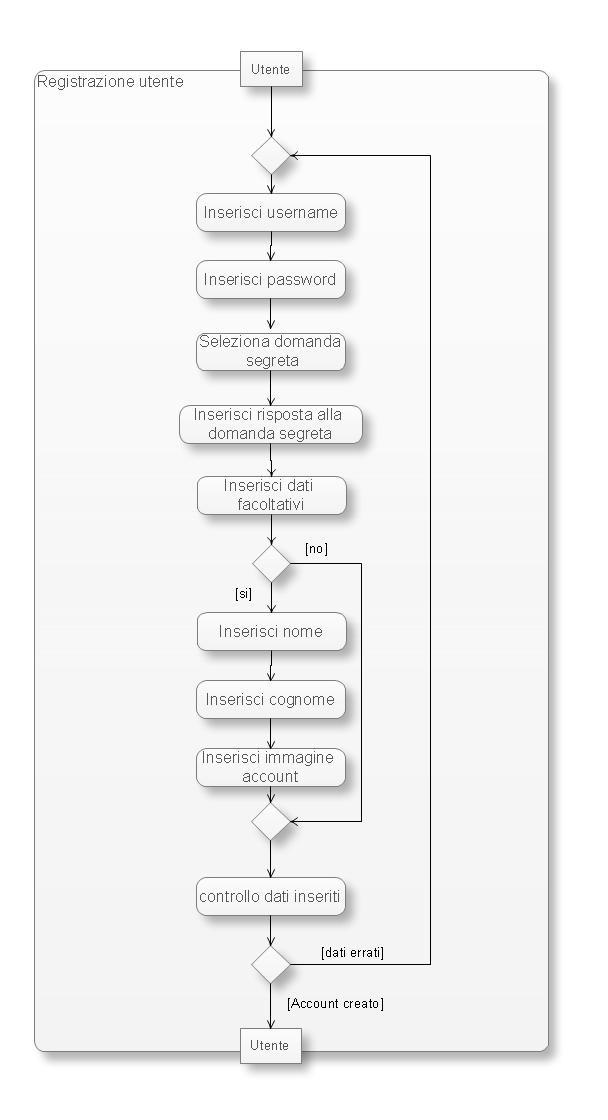
\includegraphics[width=.8\textwidth]{registrazione}
\caption{Diagramma di attività relativo alla registrazione}\label{fig:ADregistrazione}
\end{figure}

\begin{figure}[H]
\centering
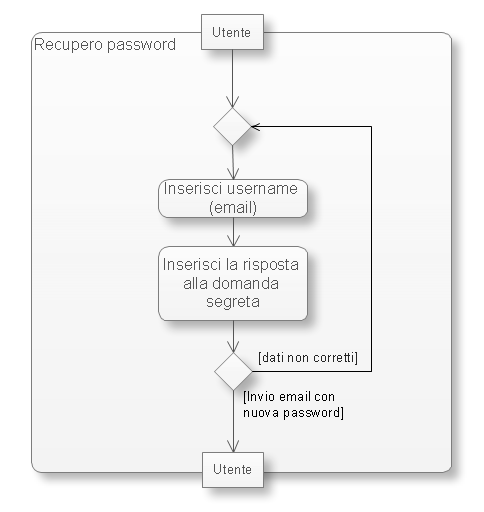
\includegraphics[width=.8\textwidth]{recupero_pass}
\caption{Diagramma di attività relativo al recupero della password}\label{fig:ADrecuperopassword}
\end{figure}


Dal diagramma principale (ricordiamo in figura \vref{fig:ADhome}) una volta autenticati è possibile raggiungere ogni funzionalità del software, come ad esempio la gestione della rubrica (figura \ref{fig:ADgestionerubrica}), la gestione del proprio account(figura \ref{fig:ADgestioneaccount}) o della segreteria (figura \ref{fig:ADgestionesegreteria}).

\begin{figure}[H]
\centering
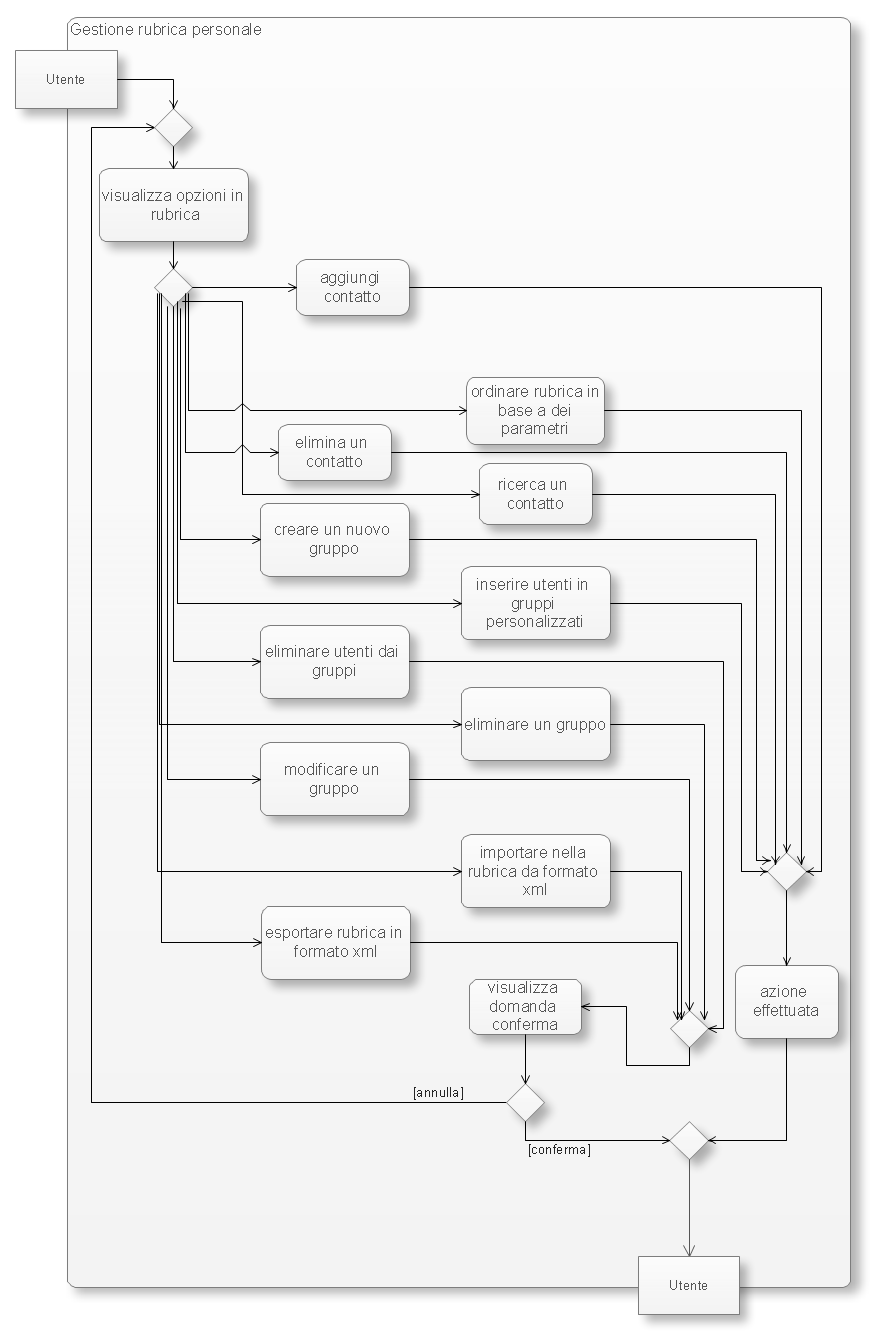
\includegraphics[width=.8\textwidth]{gestione_rub_pers}
\caption{Diagramma di attività relativo alla gestione della rubrica personale}\label{fig:ADgestionerubrica}
\end{figure}

\begin{figure}[H]
\centering
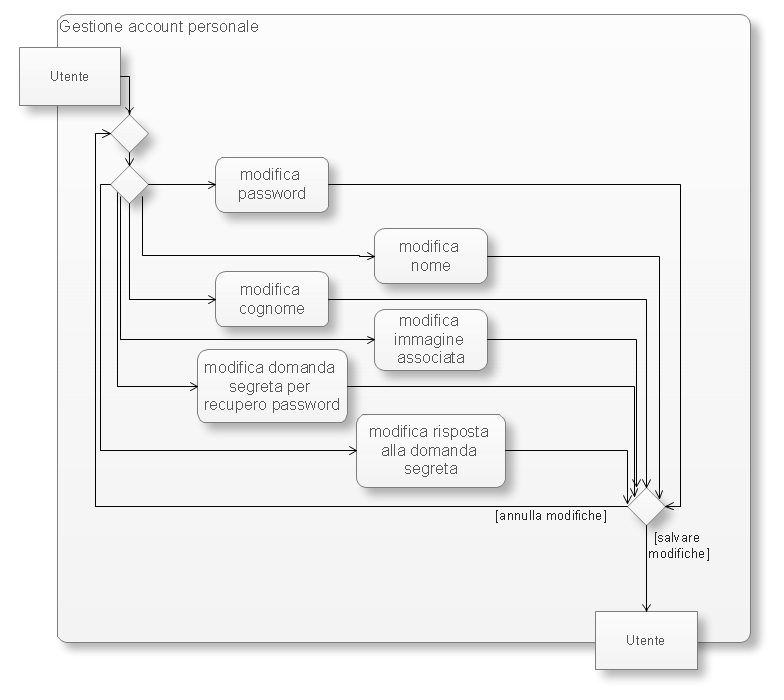
\includegraphics[width=.8\textwidth]{gestione_account_pers}
\caption{Diagramma di attività relativo alla gestione dei dati dell'account personale}\label{fig:ADgestioneaccount}
\end{figure}

\begin{figure}[H]
\centering
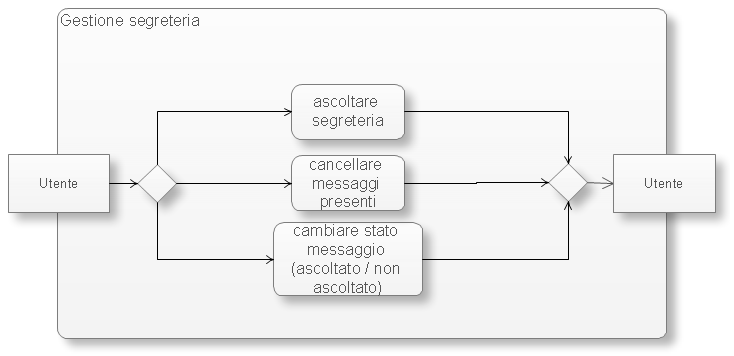
\includegraphics[width=.8\textwidth]{gestione_segreteria}
\caption{Diagramma di attività relativo alla gestione della segretria}\label{fig:ADgestionesegreteria}
\end{figure}


\`{E} infine data la possibilità di connettersi con altri utenti tramite l'attività connessione illustrata nel dettaglio in figura \ref{fig:ADconnessione}.

\begin{figure}[H]
\centering
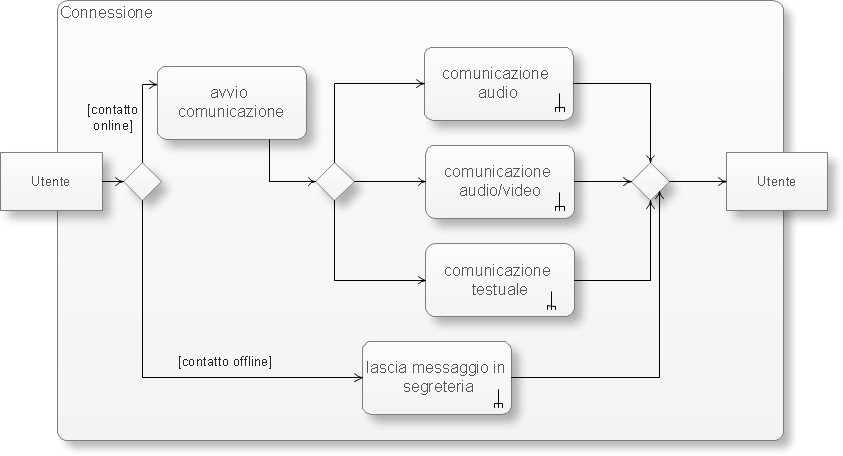
\includegraphics[width=.8\textwidth]{connessione}
\caption{Diagramma di attività relativo alla connessione}\label{fig:ADconnessione}
\end{figure}

La connessione può essere di tipo audio (figura \ref{fig:ADcomaudio}), audio/video (figura \ref{fig:ADcomaudiovideo}) o testuale (figura \ref{fig:ADcomtestuale}). In tutte e tre le tipologie di connessione è possibile effettuare una condivisione di risorse, come specificato in figura \ref{fig:ADcondrisorse}, o registrare una chiamata (tranne nel caso di comunicazione testuale) figura \ref{fig:ADregistrachiamata}.

\begin{figure}[H]
\centering
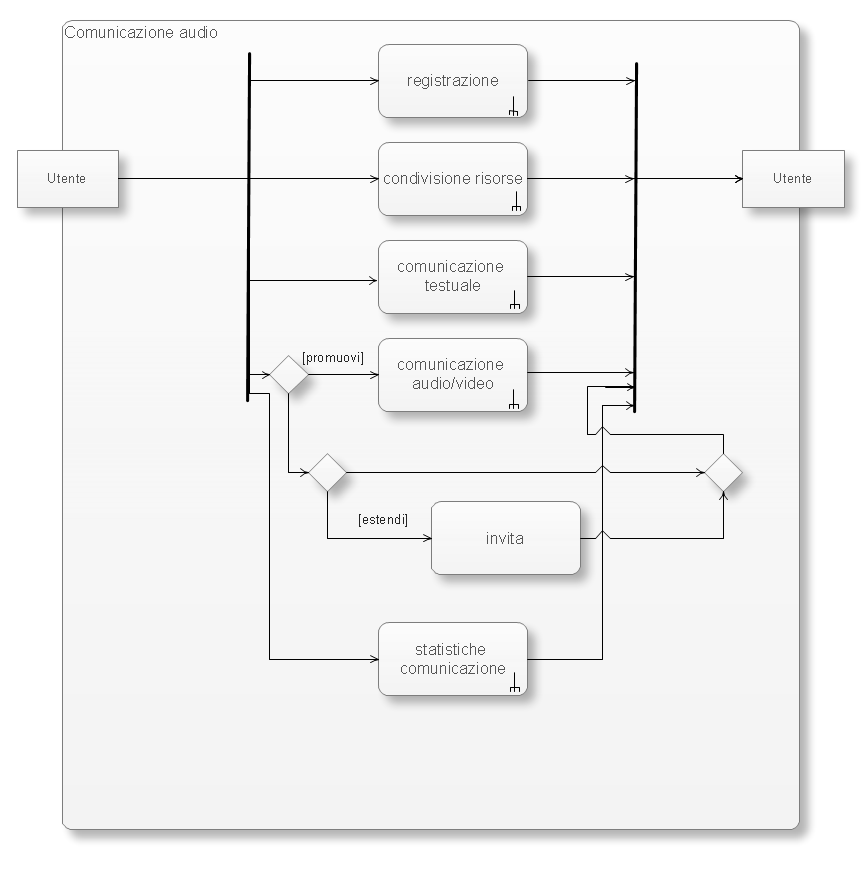
\includegraphics[width=1\textwidth]{com_audio}
\caption{Diagramma di attività relativo alla comunicazione audio}\label{fig:ADcomaudio}
\end{figure}

\begin{figure}[H]
\centering
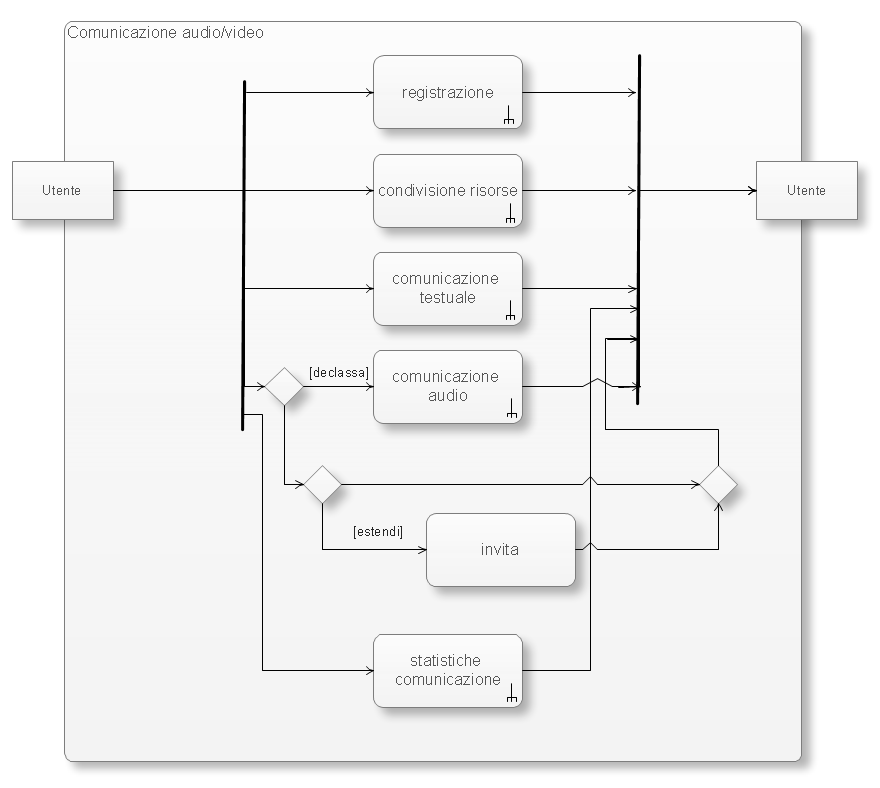
\includegraphics[width=.8\textwidth]{com_audiovideo}
\caption{Diagramma di attività relativo alla comunicazione audio/video}\label{fig:ADcomaudiovideo}
\end{figure}

\begin{figure}[H]
\centering
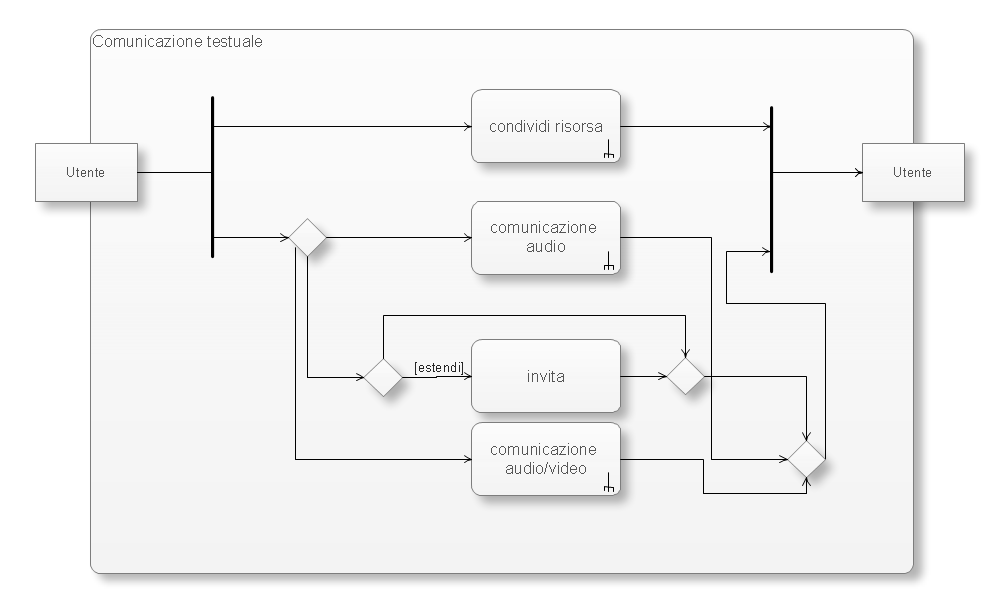
\includegraphics[width=.8\textwidth]{com_testuale}
\caption{Diagramma di attività relativo alla comunicazione testuale}\label{fig:ADcomtestuale}
\end{figure}

\begin{figure}[H]
\centering
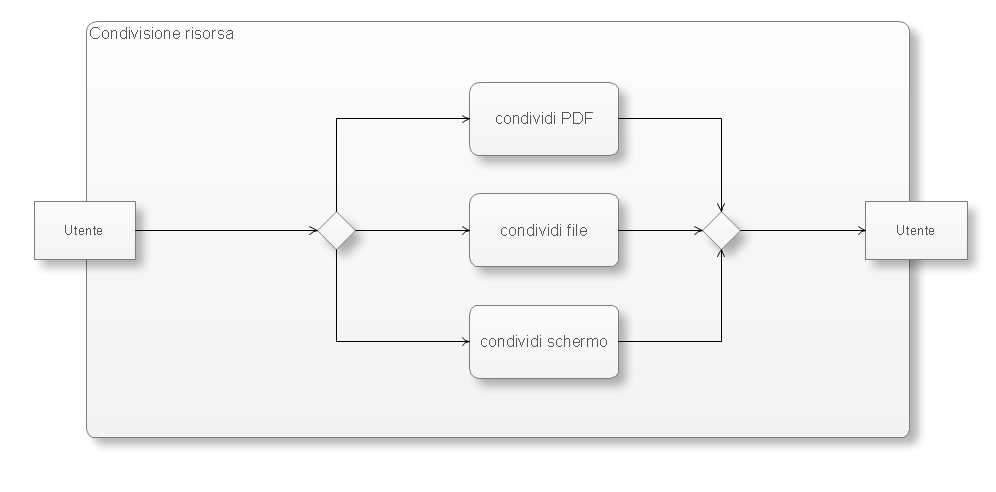
\includegraphics[width=.8\textwidth]{condividi_ris}
\caption{Diagramma di attività relativo alla condivisione di risorse}\label{fig:ADcondrisorse}
\end{figure}

\begin{figure}[H]
\centering
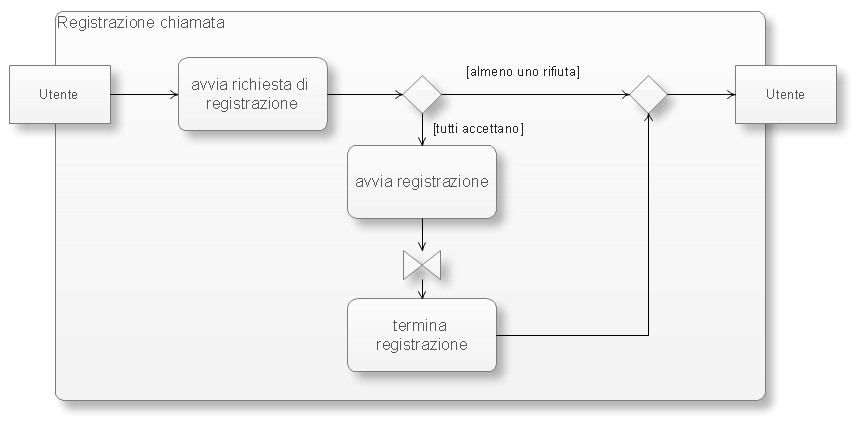
\includegraphics[width=.8\textwidth]{registrazione_chiamata}
\caption{Diagramma di attività relativo alla registrazione della chiamata}\label{fig:ADregistrachiamata}
\end{figure}

In conclusione si ricorda che è possibile lasciare un messaggio nella segreteria di un determinato contatto se non presente in linea nel momento in cui desideriamo comunicare con lui \ref{fig:ADmessegreteria}.

\begin{figure}[H]
\centering
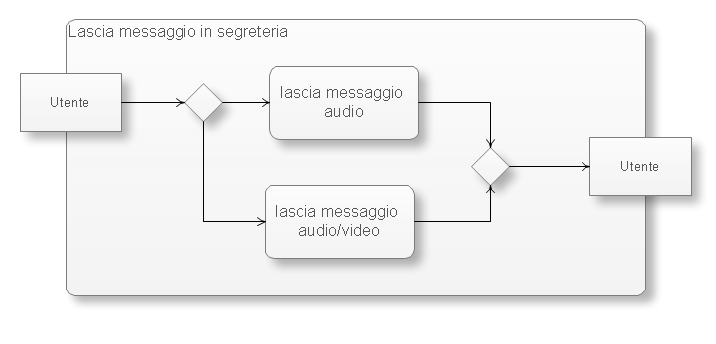
\includegraphics[width=.8\textwidth]{mes_segreteria}
\caption{Diagramma di attività relativo alla memorizzazione di un messaggio in segreteria}\label{fig:ADmessegreteria}
\end{figure}

\clearpage

\section{Tracciamenti}\label{sec:tracciamenti}
Nella seguente sezione vengono proposti tutti i tracciamenti eseguiti mediante il sistema Synthsis Requirment Manager. I tracciamenti proposti sono giustificati dalle seguenti due motivazioni:

\begin{itemize}
	\item Dimostrare il soddisfacimento per necessarietà e sufficienza della corrispondenza tra gli elementi tracciati (e.g. un componente deve rispondere necessariamente alle esigenze di uno o più requisiti, tali insomma che ne giustifichino l'esistenza. D'altro canto è richiesto che ogni requisito definito in fase d'analisi sia soddisfatto e risolto da almeno un componente).
	\item dare una lettura generale delle varie: componenti, requisiti, \underline{design pattern} e classi.
\end{itemize}

\newpage\section{Diagrammi dei casi d'uso}

\subsection{UC1: Login e registrazione}
\begin{figure}[H]
\begin{center}
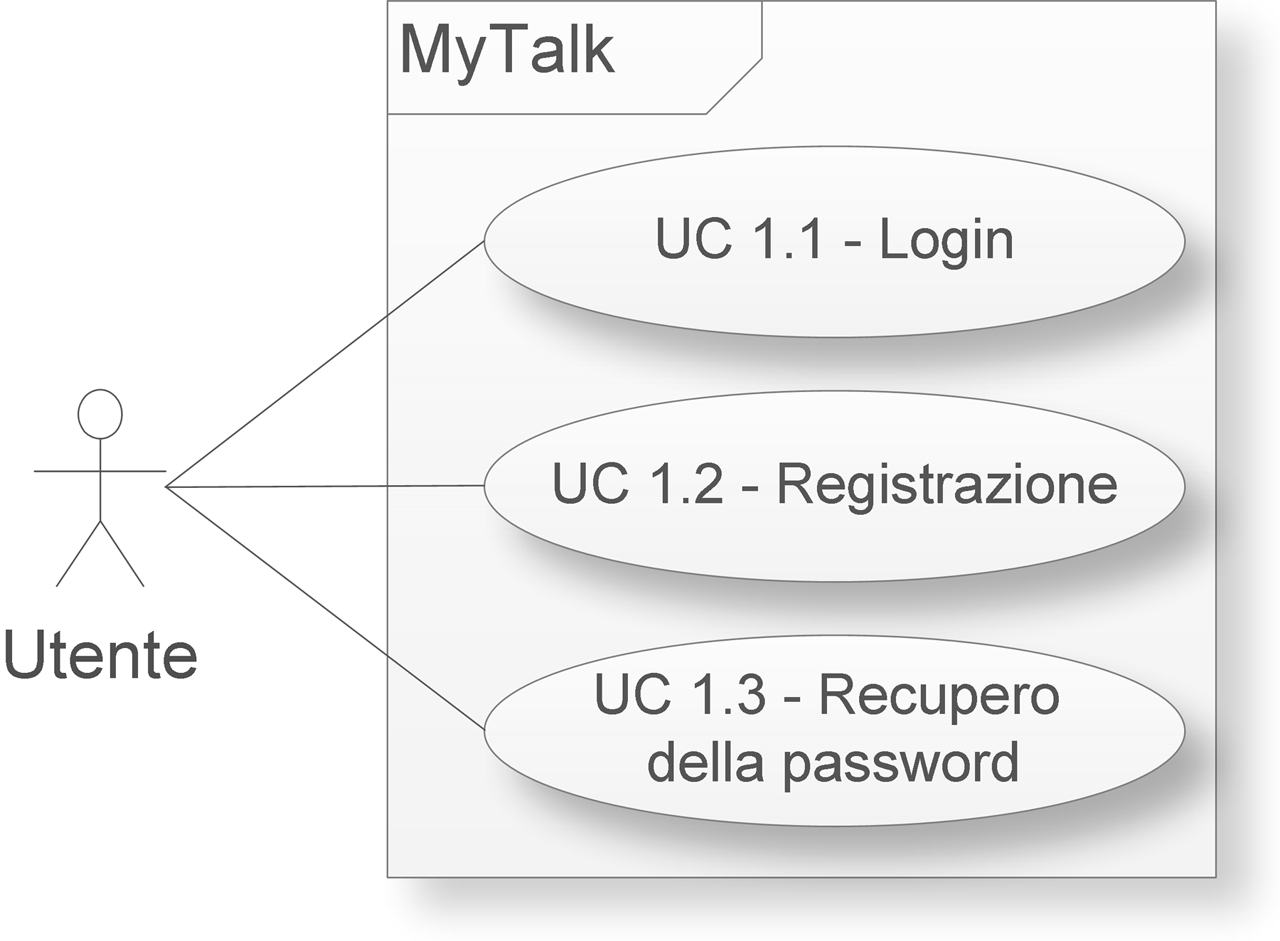
\includegraphics[width=.8\textwidth]{UC1}
\caption{}\label{fig:}
\end{center}
\end{figure}
\begin{description}
\item{\scshape\bfseries Attori principali:}Utente.
\item{\scshape\bfseries Scopo e descrizione:} L'utente può effettuare l'accesso al sistema mediante la procedura di autenticazione se registrato (UC1.1), recuperare la password dimenticata (UC1.3) oppure può provvedere alla propria registrazione (UC1.2), quindi effettuare successivamente l'accesso al sistema (UC1.1).
\item{\scshape\bfseries Precondizione:} Il sistema MyTalk è attivo e funzionante, le infrastrutture di rete sono attive.
\item{\scshape\bfseries Postcondizione:} L'utente si trova in uno di questi casi: ha avviato la procedura per l'autenticazione al sistema (UC1.1), oppure ha avviato la procedura per per la registrazione nel sistema (UC1.2), oppure ha avviato la procedura per il recupero della password dimenticata (UC1.3).
\item{\scshape\bfseries Illustrazione scenario principale:} L'utente può decidere di avviare la procedura di autenticazione al sistema (UC1.1), altrimenti se non ricorda le credenziali, può avviare la procedura per il recupero della password (UC1.3). Invece se l'utente sa di non essere registrato nel sistema, può avviare la procedura di registrazione (UC1.2).
\end{description}

\subsection{UC1.1: Login utente}
\begin{figure}[H]
\begin{center}
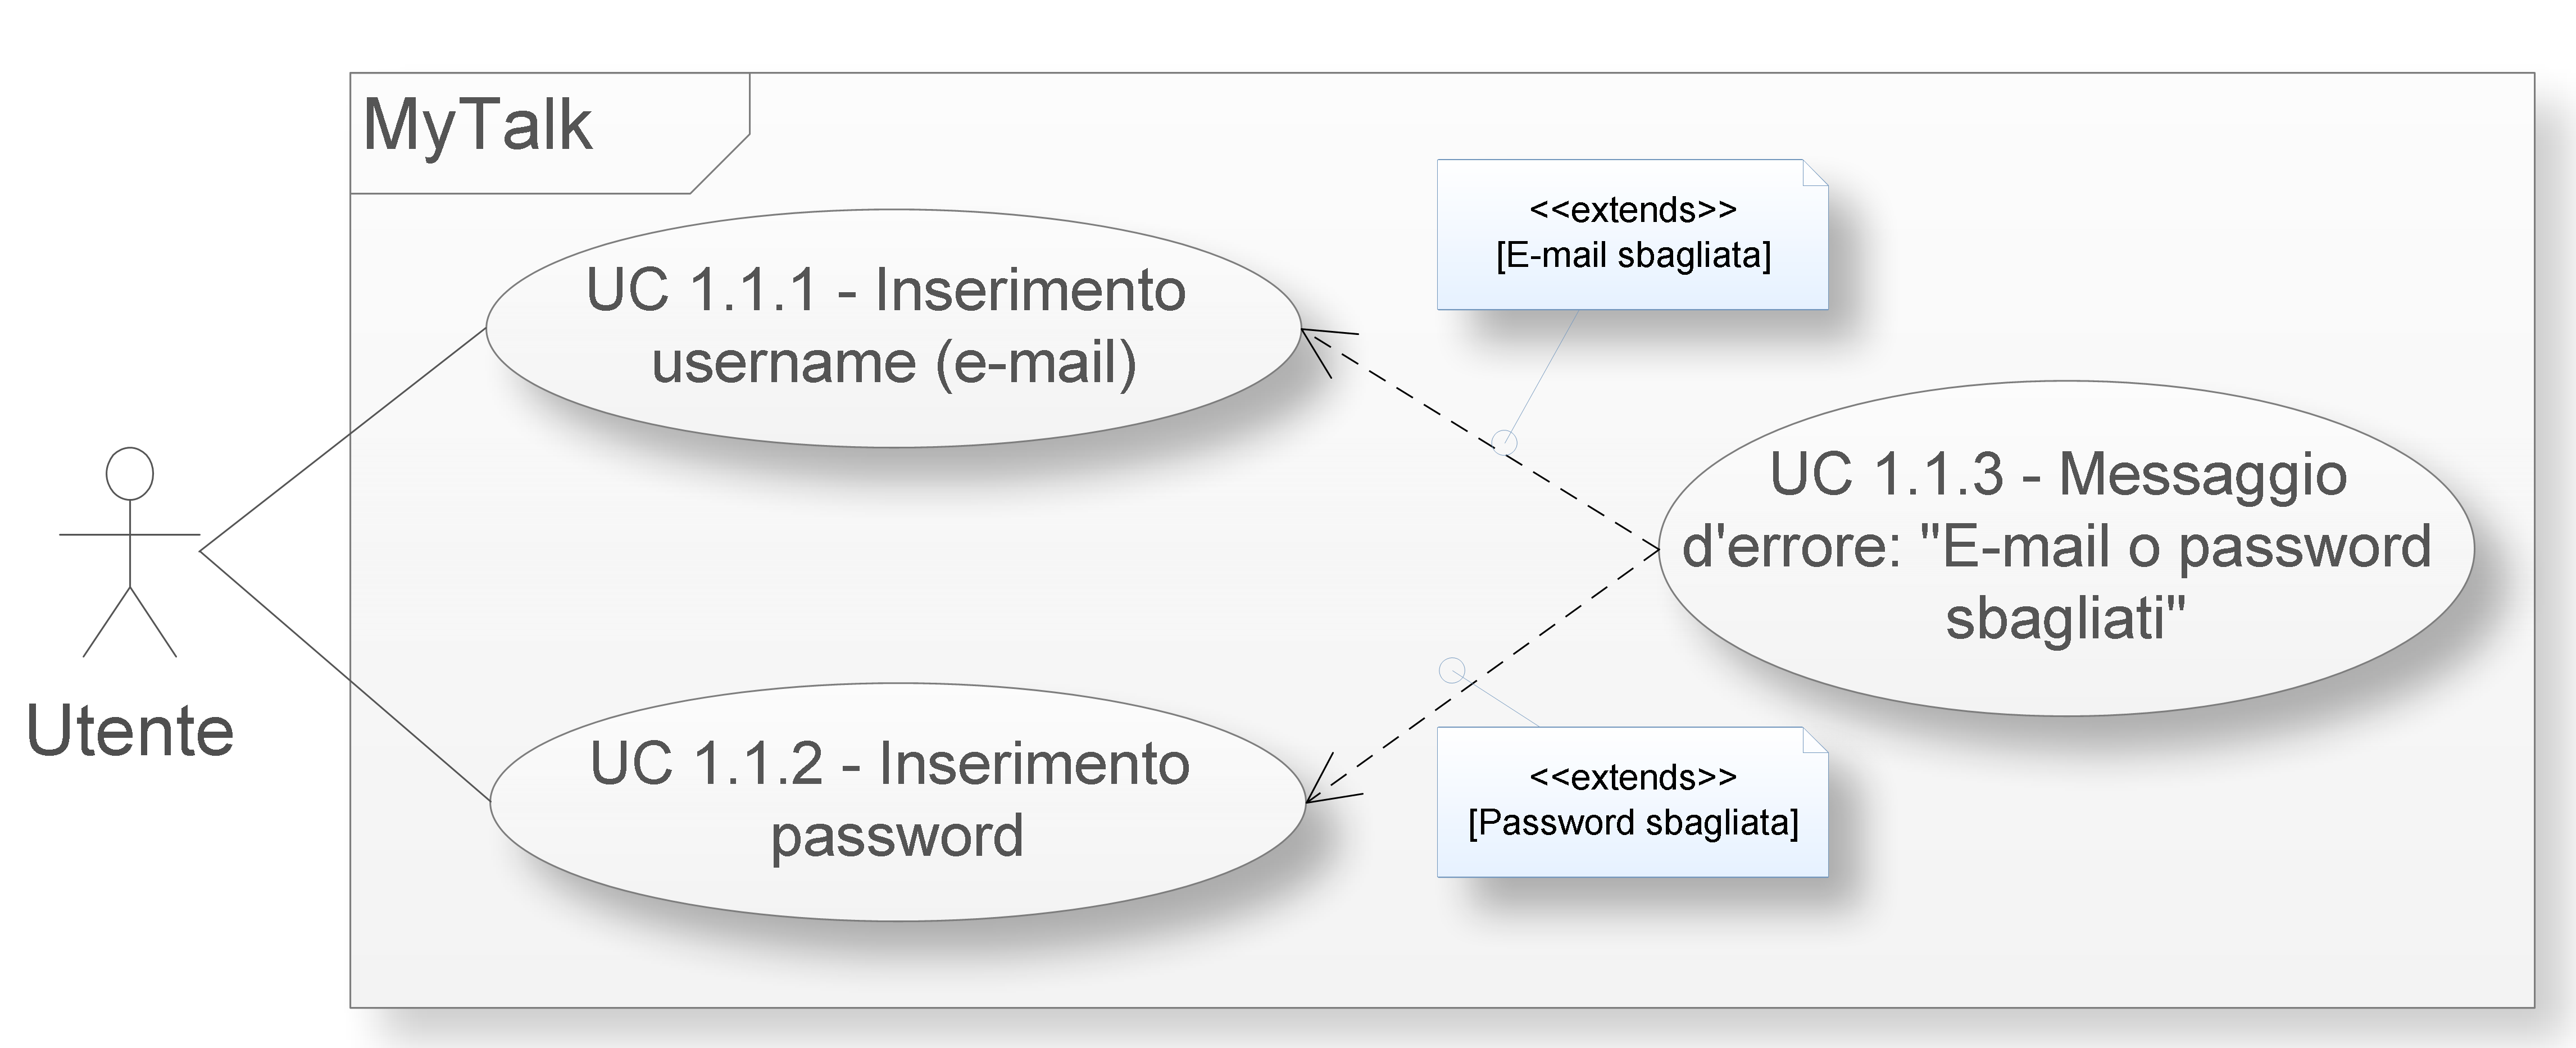
\includegraphics[width=.8\textwidth]{UC1-1}
\caption{}\label{fig:}
\end{center}
\end{figure}
\begin{description}
\item{\scshape\bfseries Attori principali:}Utente.
\item{\scshape\bfseries Scopo e descrizione:} L'utente si autentica per accedere al sistema MyTalk
\item{\scshape\bfseries Precondizione:} L'utente (generico) visualizza la schermata iniziale e il sistema è pronto.
\item{\scshape\bfseries Postcondizione:} L'utente è autenticato nel sistema
\item{\scshape\bfseries Illustrazione scenario principale:} L'utente inserisce username (UC1.1.1) e password (UC1.1.2) corretti e conferma.
\item{\scshape\bfseries Illustrazione scenario alternativo:} L'utente ha inserito dati non corretti: il sistema lo notifica con un errore unico (UC1.1.3) e rimane in attesa di una correzione. (Non vengono visualizzati due errori separati ma un errore unico generico per aumentare la sicurezza).
\end{description}

\subsection{UC1.2: Registrazione}
\begin{figure}[H]
\begin{center}
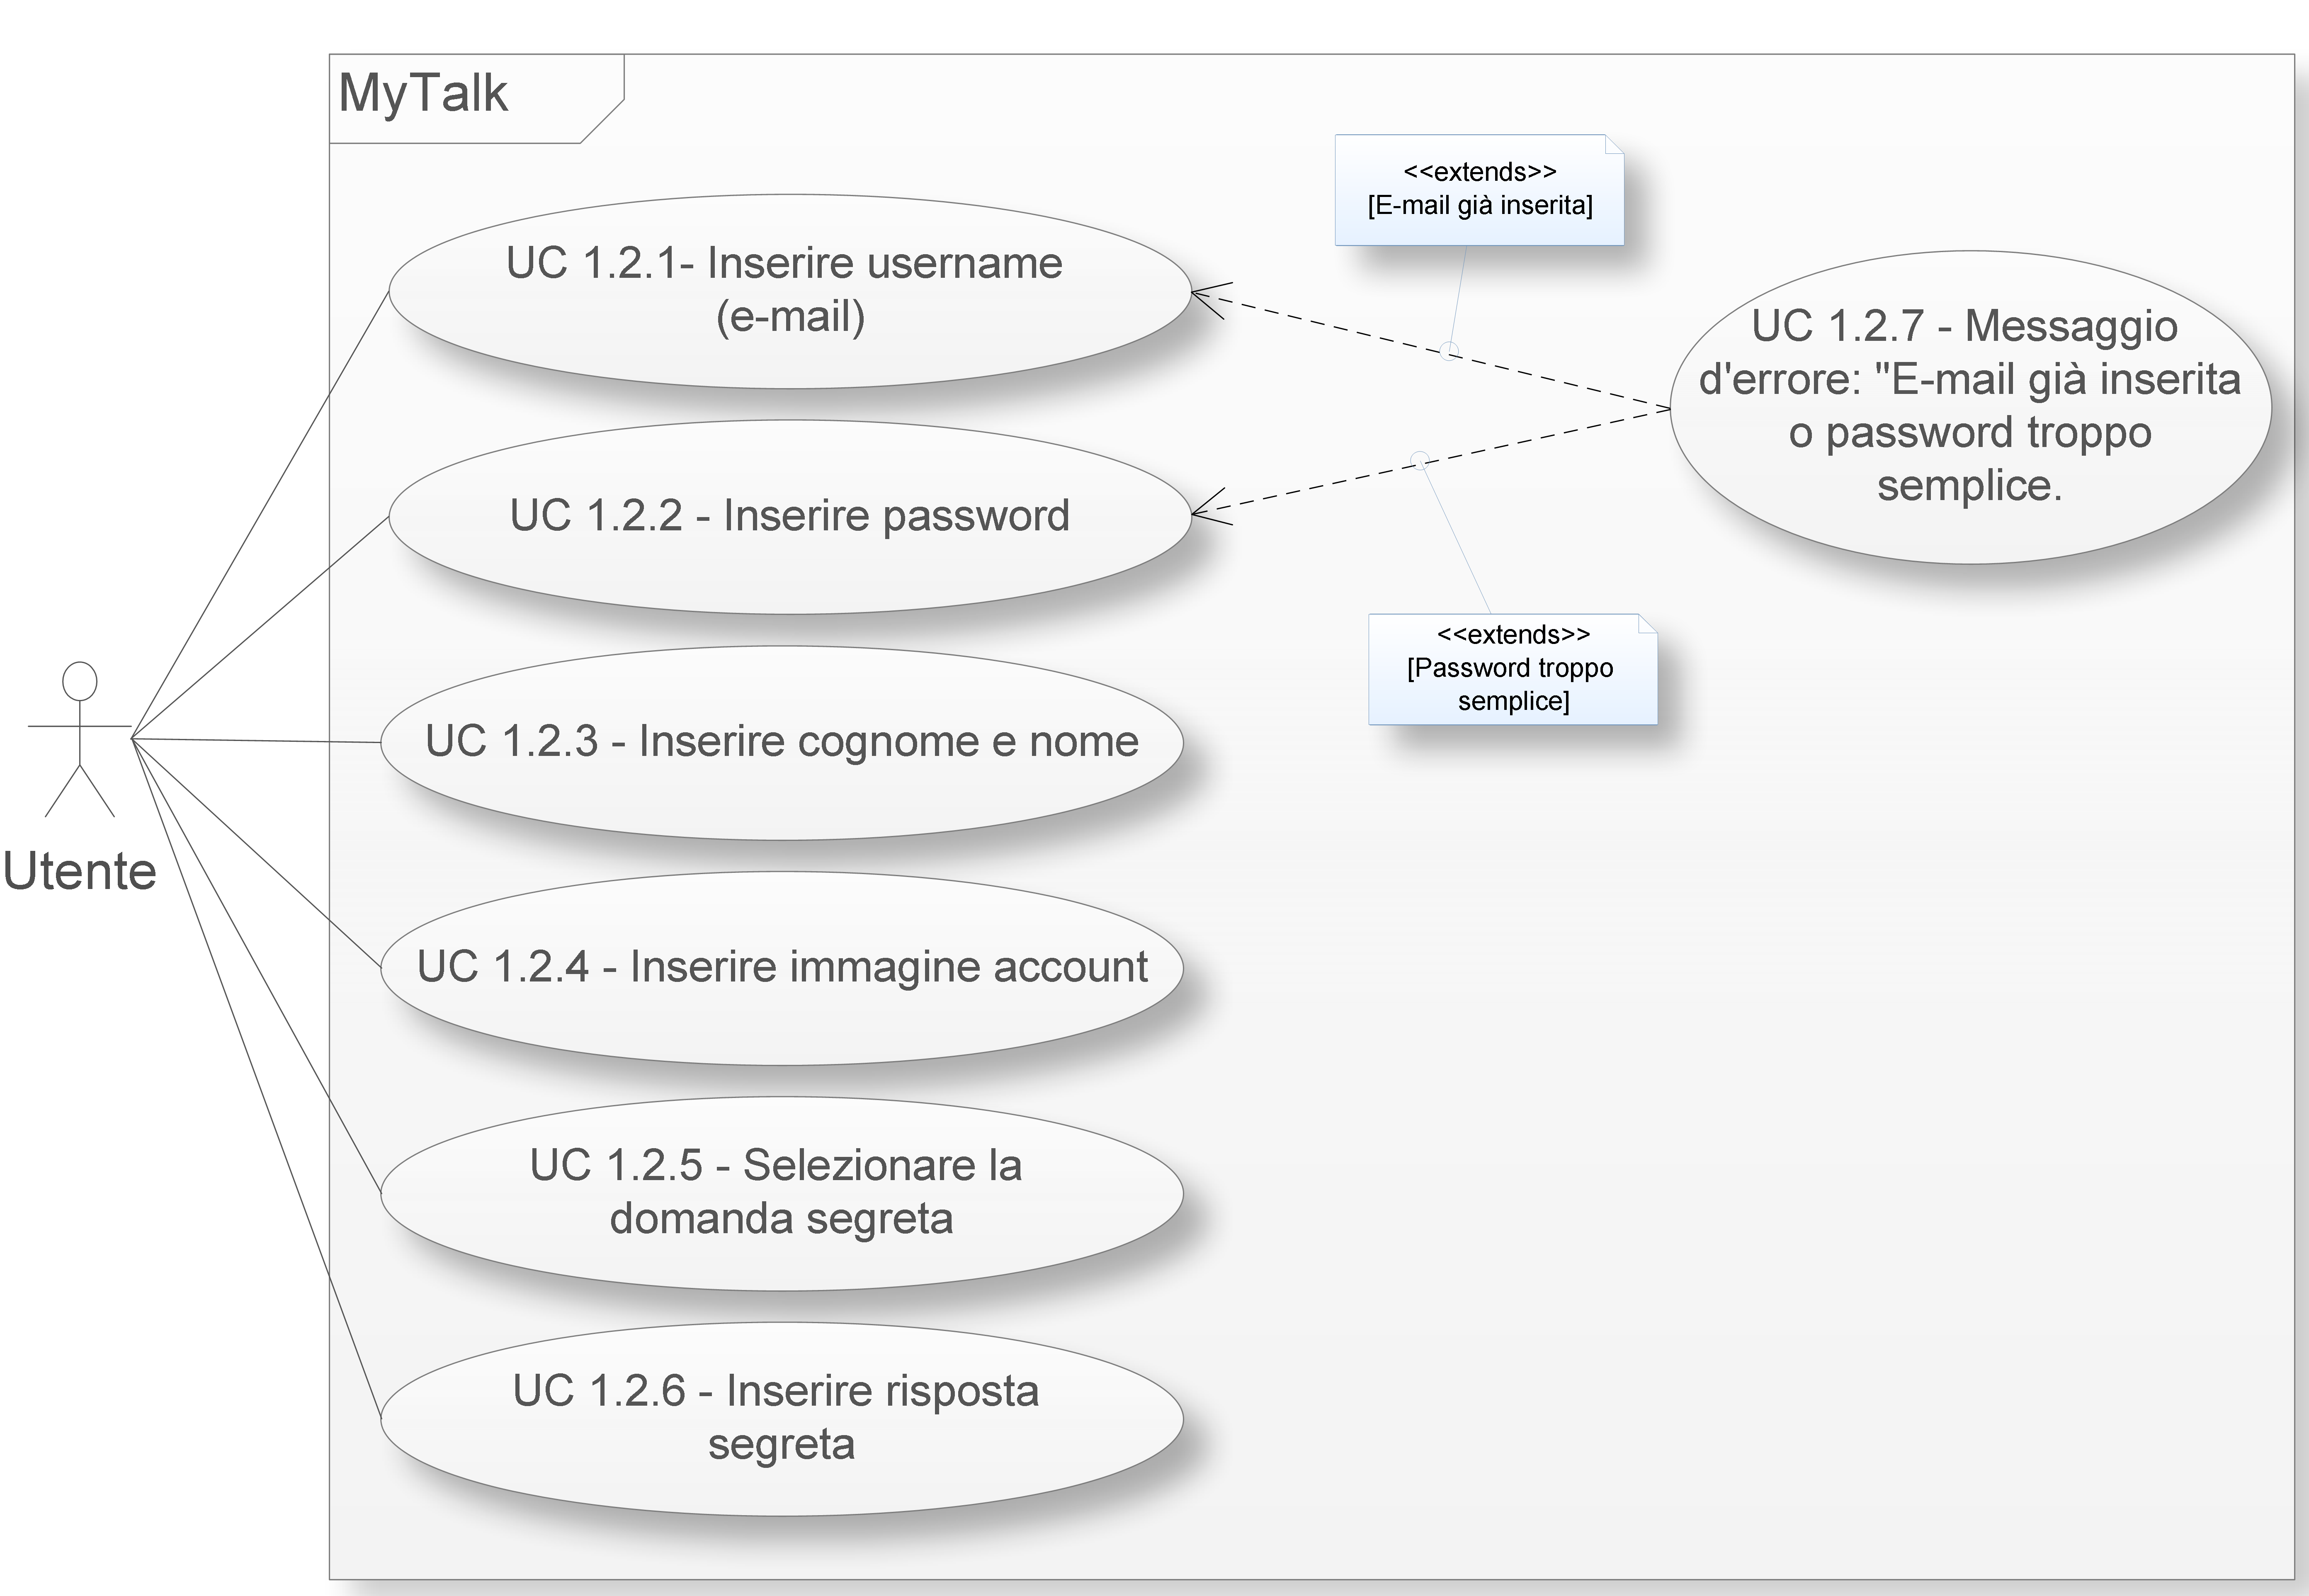
\includegraphics[width=.8\textwidth]{UC1-2}
\caption{}\label{fig:}
\end{center}
\end{figure}
\begin{description}
\item{\scshape\bfseries Attori principali:}Utente.
\item{\scshape\bfseries Scopo e descrizione:} L'utente si registra nel sistema.
\item{\scshape\bfseries Precondizione:} L'utente (generico) visualizza la schermata iniziale e il sistema è pronto.
\item{\scshape\bfseries Postcondizione:} L'utente si è registrato nel sistema MyTalk
\item{\scshape\bfseries Illustrazione scenario principale:} La registrazione di un nuovo account comporta l'inserimento di un indirizzo email come ID utente (UC1.2.1), una password (UC1.2.2), domanda segreta (UC1.2.6) e la relativa risposta (UC1.2.7). Il nome (UC1.2.3), il cognome (UC1.2.4) e un'immagine (UC1.2.5) da associare al proprio profilo possono essere inserite facoltativamente. Per andare a buon fine la procedura di registrazione richiede che la password prescelta assicuri un sufficiente livello di complessità e prevede altresì la selezione della domanda segreta (e della relativa risposta) necessarie al recupero della password in caso di smarrimento, nonché la validazione dell''indirizzo email al fine di verificare che l''utente ne sia effettivamente in possesso.
\item{\scshape\bfseries Illustrazione scenario alternativo:} Il sistema può fallire per via dell'inserimento di dati non corretti. Il sistema mostra un errore relativo all'username (UC1.2.8) oppure alla password (UC1.2.9)
\end{description}

\subsection{UC1.3: Recupero della password}
\begin{figure}[H]
\begin{center}
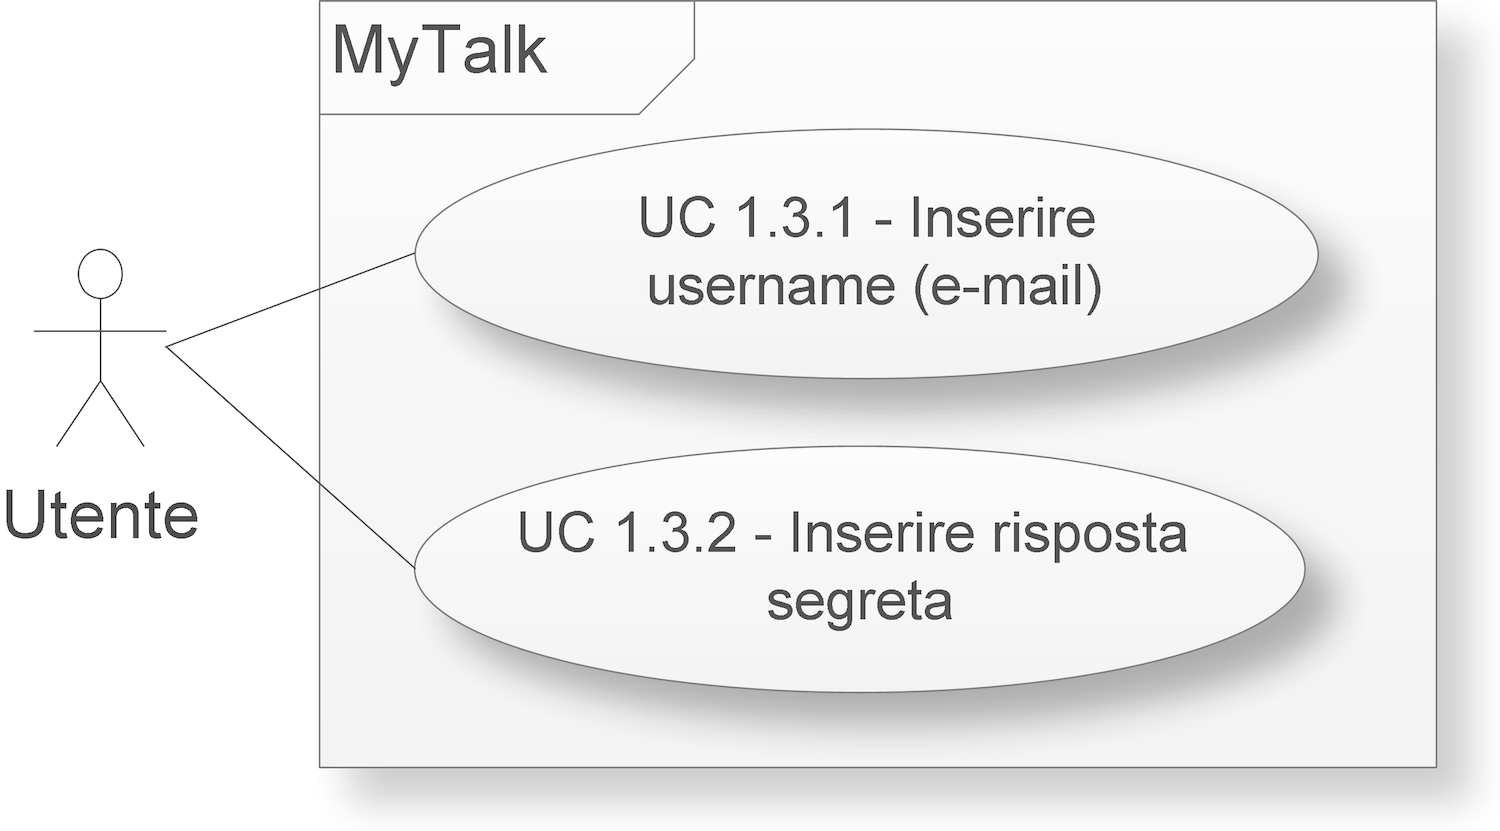
\includegraphics[width=.8\textwidth]{UC1-3}
\caption{}\label{fig:}
\end{center}
\end{figure}
\begin{description}
\item{\scshape\bfseries Attori principali:}Utente.
\item{\scshape\bfseries Scopo e descrizione:} L'utente desidera recuperare la password smarrita.
\item{\scshape\bfseries Precondizione:} L'utente (generico) visualizza la schermata iniziale e il sistema è pronto.
\item{\scshape\bfseries Postcondizione:} L'utente riceve per e-mail la password dimenticata.
\item{\scshape\bfseries Illustrazione scenario principale:} Si avvia la procedura di recupero della password: l'utente deve inserire l'e-mail (UC1.3.1) e la risposta alla domanda segreta (UC1.3.2). A questo segue l'invio della password all'indirizzo email indicato in fase di registrazione.
\item{\scshape\bfseries Illustrazione scenario alternativo:} Il sistema può fallire per via dell'inserimento di dati non corretti. Il sistema evidenzia gli errori e rimane in attesa della correzione.
\end{description}

\subsection{UC2: Home screen dell'applicativo}
\begin{figure}[H]
\begin{center}
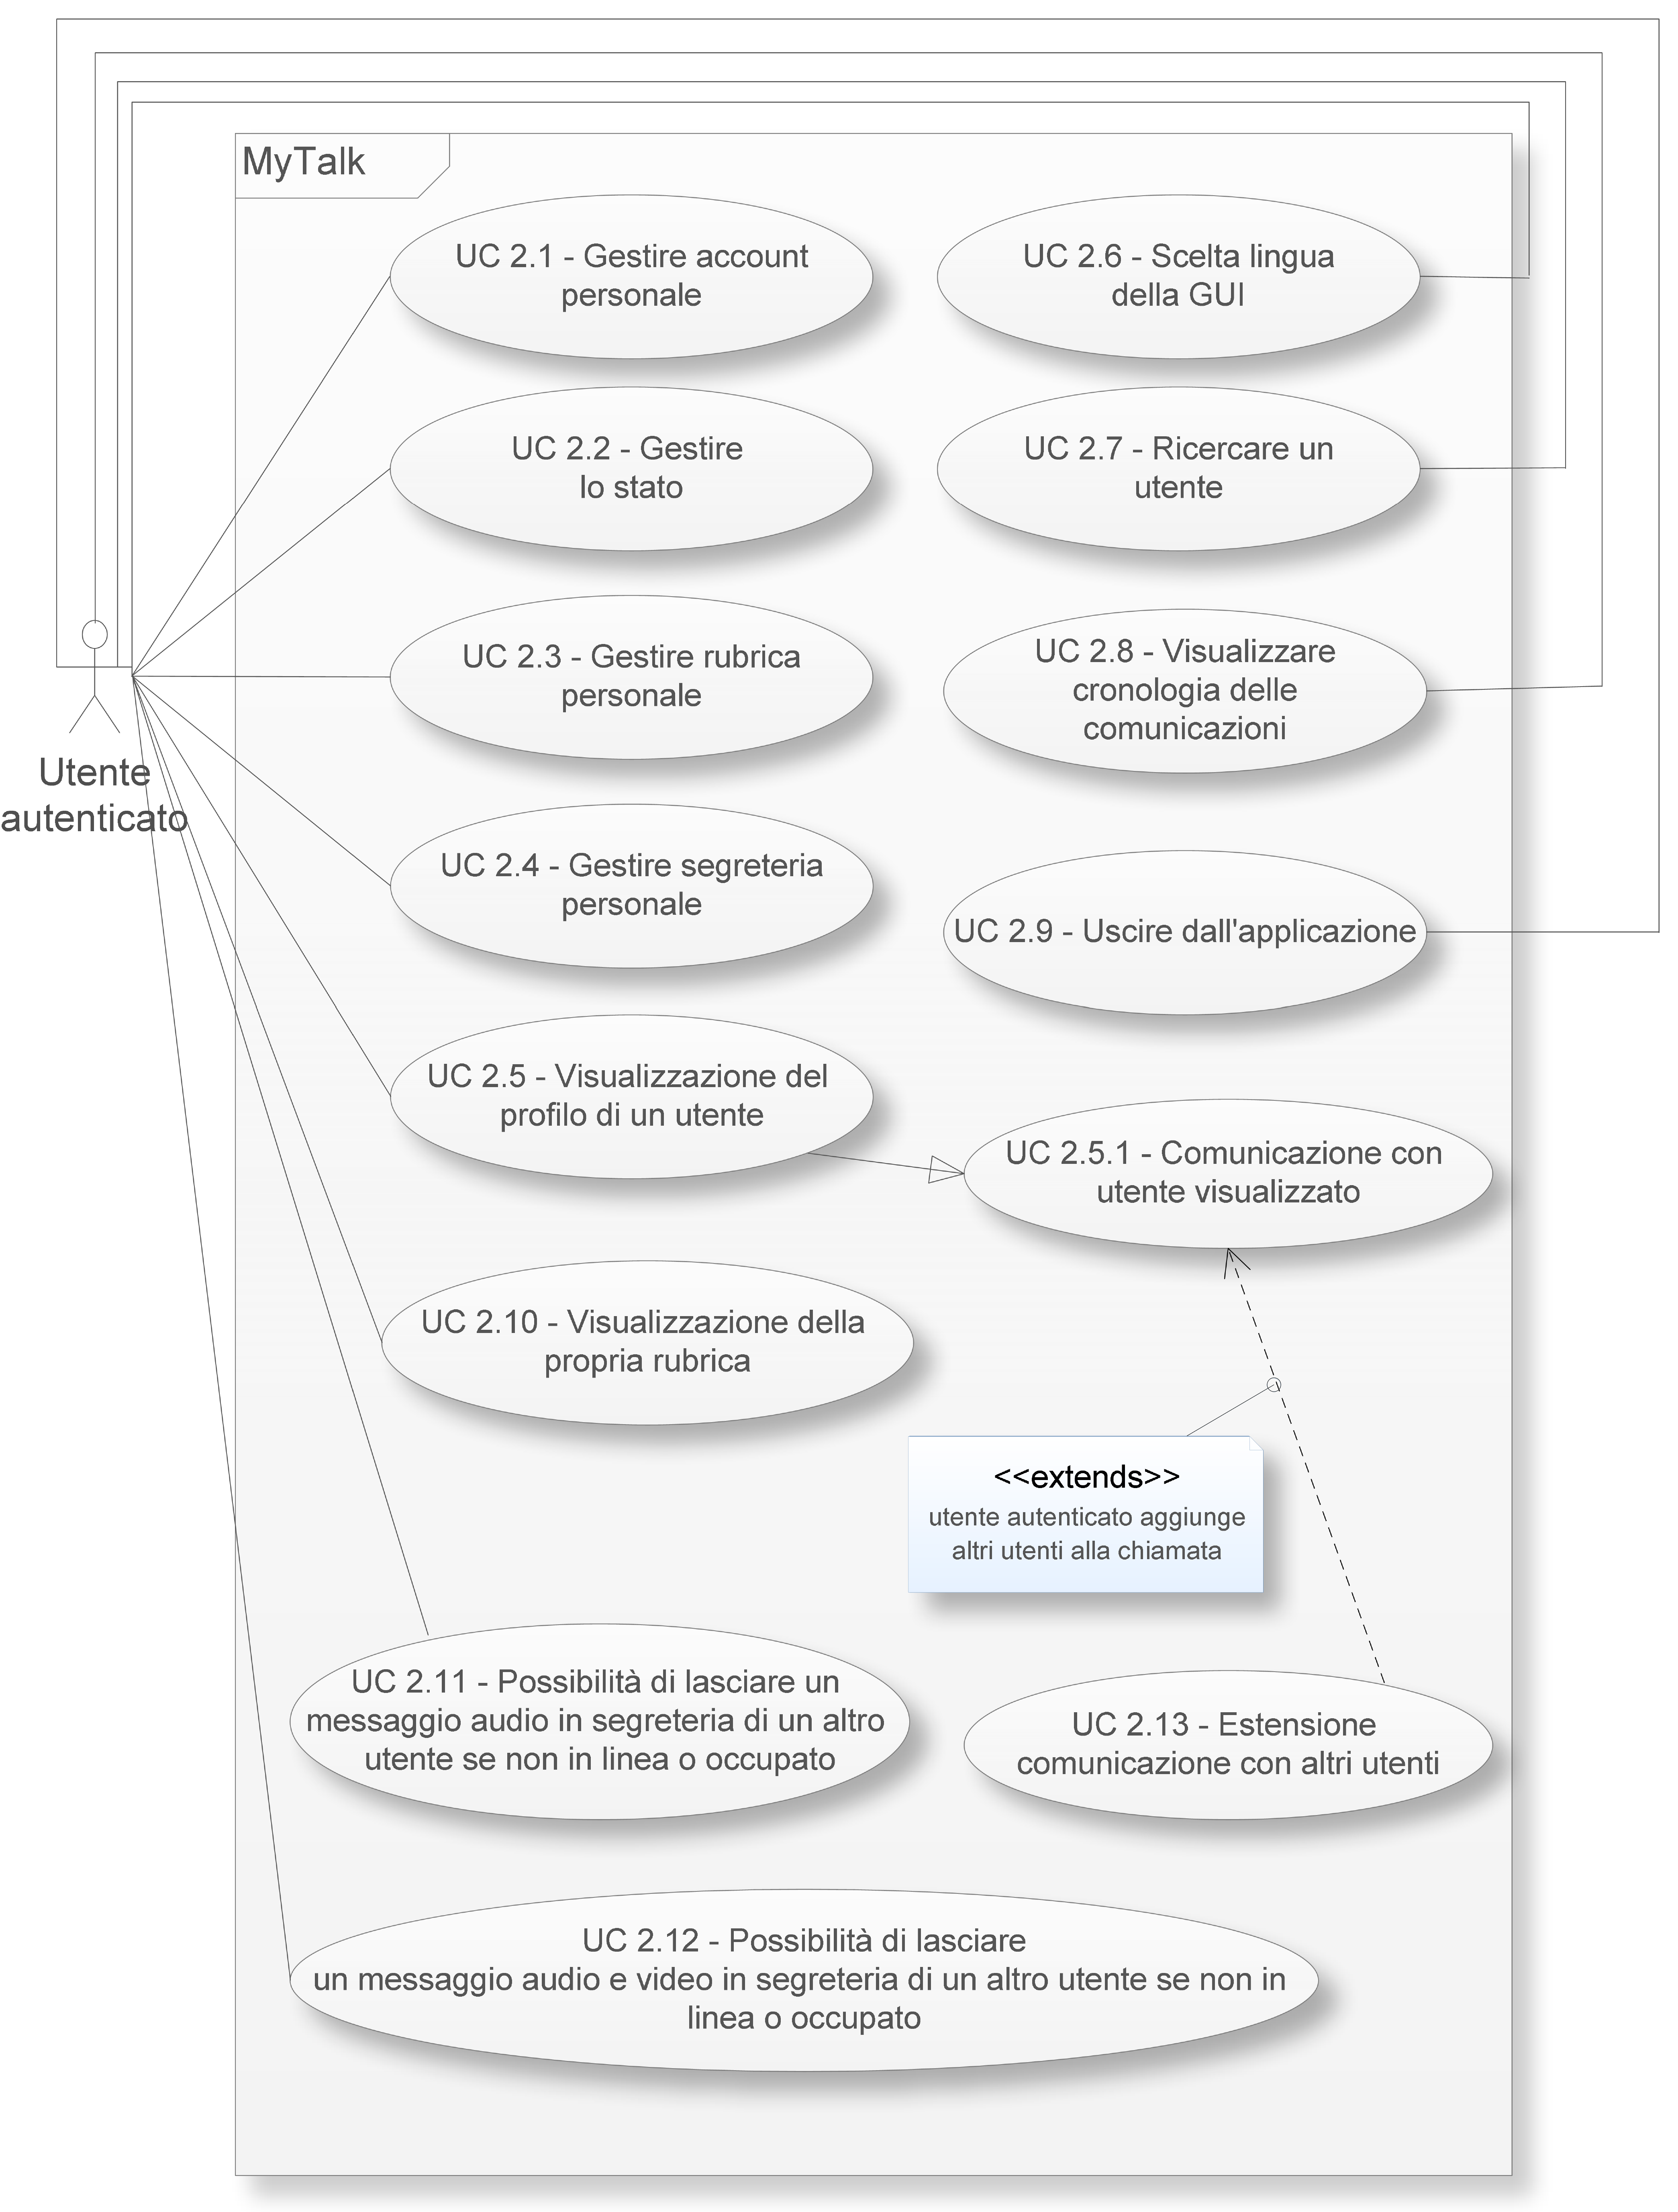
\includegraphics[width=.8\textwidth]{UC2}
\caption{}\label{fig:}
\end{center}
\end{figure}
\begin{description}
\item{\scshape\bfseries Attori principali:}Utente autenticato.
\item{\scshape\bfseries Scopo e descrizione:} Funzionalità generali offerte all'utente autenticato e presenti nella Home screen dell'applicativo.
\item{\scshape\bfseries Precondizione:} L'utente ha effettuato il login ed è autenticato nel sistema.
\item{\scshape\bfseries Postcondizione:} L'utente ha eseguito una delle funzioni proposte.
\item{\scshape\bfseries Illustrazione scenario principale:} L'utente dopo aver eseguito il login al sistema, si trova nella Home dell'applicativo. Qui può svolgere una delle seguenti operazioni: gestire il proprio account (UC2.1), scegliere la lingua della GUI (UC2.6), gestire lo stato (UC2.2), eseguire delle ricerche di utenti (UC2.7), gestire la propria rubrica (UC2.3), lasciare un messaggio nella segreteria di un utente se esso non è in linea o è occupato (UC2.11 - UC2.12), gestire la propria segreteria (UC2.4), visualizzare la cronologia delle comunicazioni (UC2.8), visualizzare la propria rubrica (UC2.10) e visualizzare il profilo di un utente (UC2.5) dopo averlo selezionato da una lista. Infine l'utente ha la possibilità di chiudere l'applicativo (UC2.9).
\item{\scshape\bfseries Illustrazione scenario alternativo:} L'utente, se ha già avviato una connessione con un altro utente, può estenderla con altri (UC2.12).
\end{description}

\subsection{UC2.1: Gestione account}
\begin{figure}[H]
\begin{center}
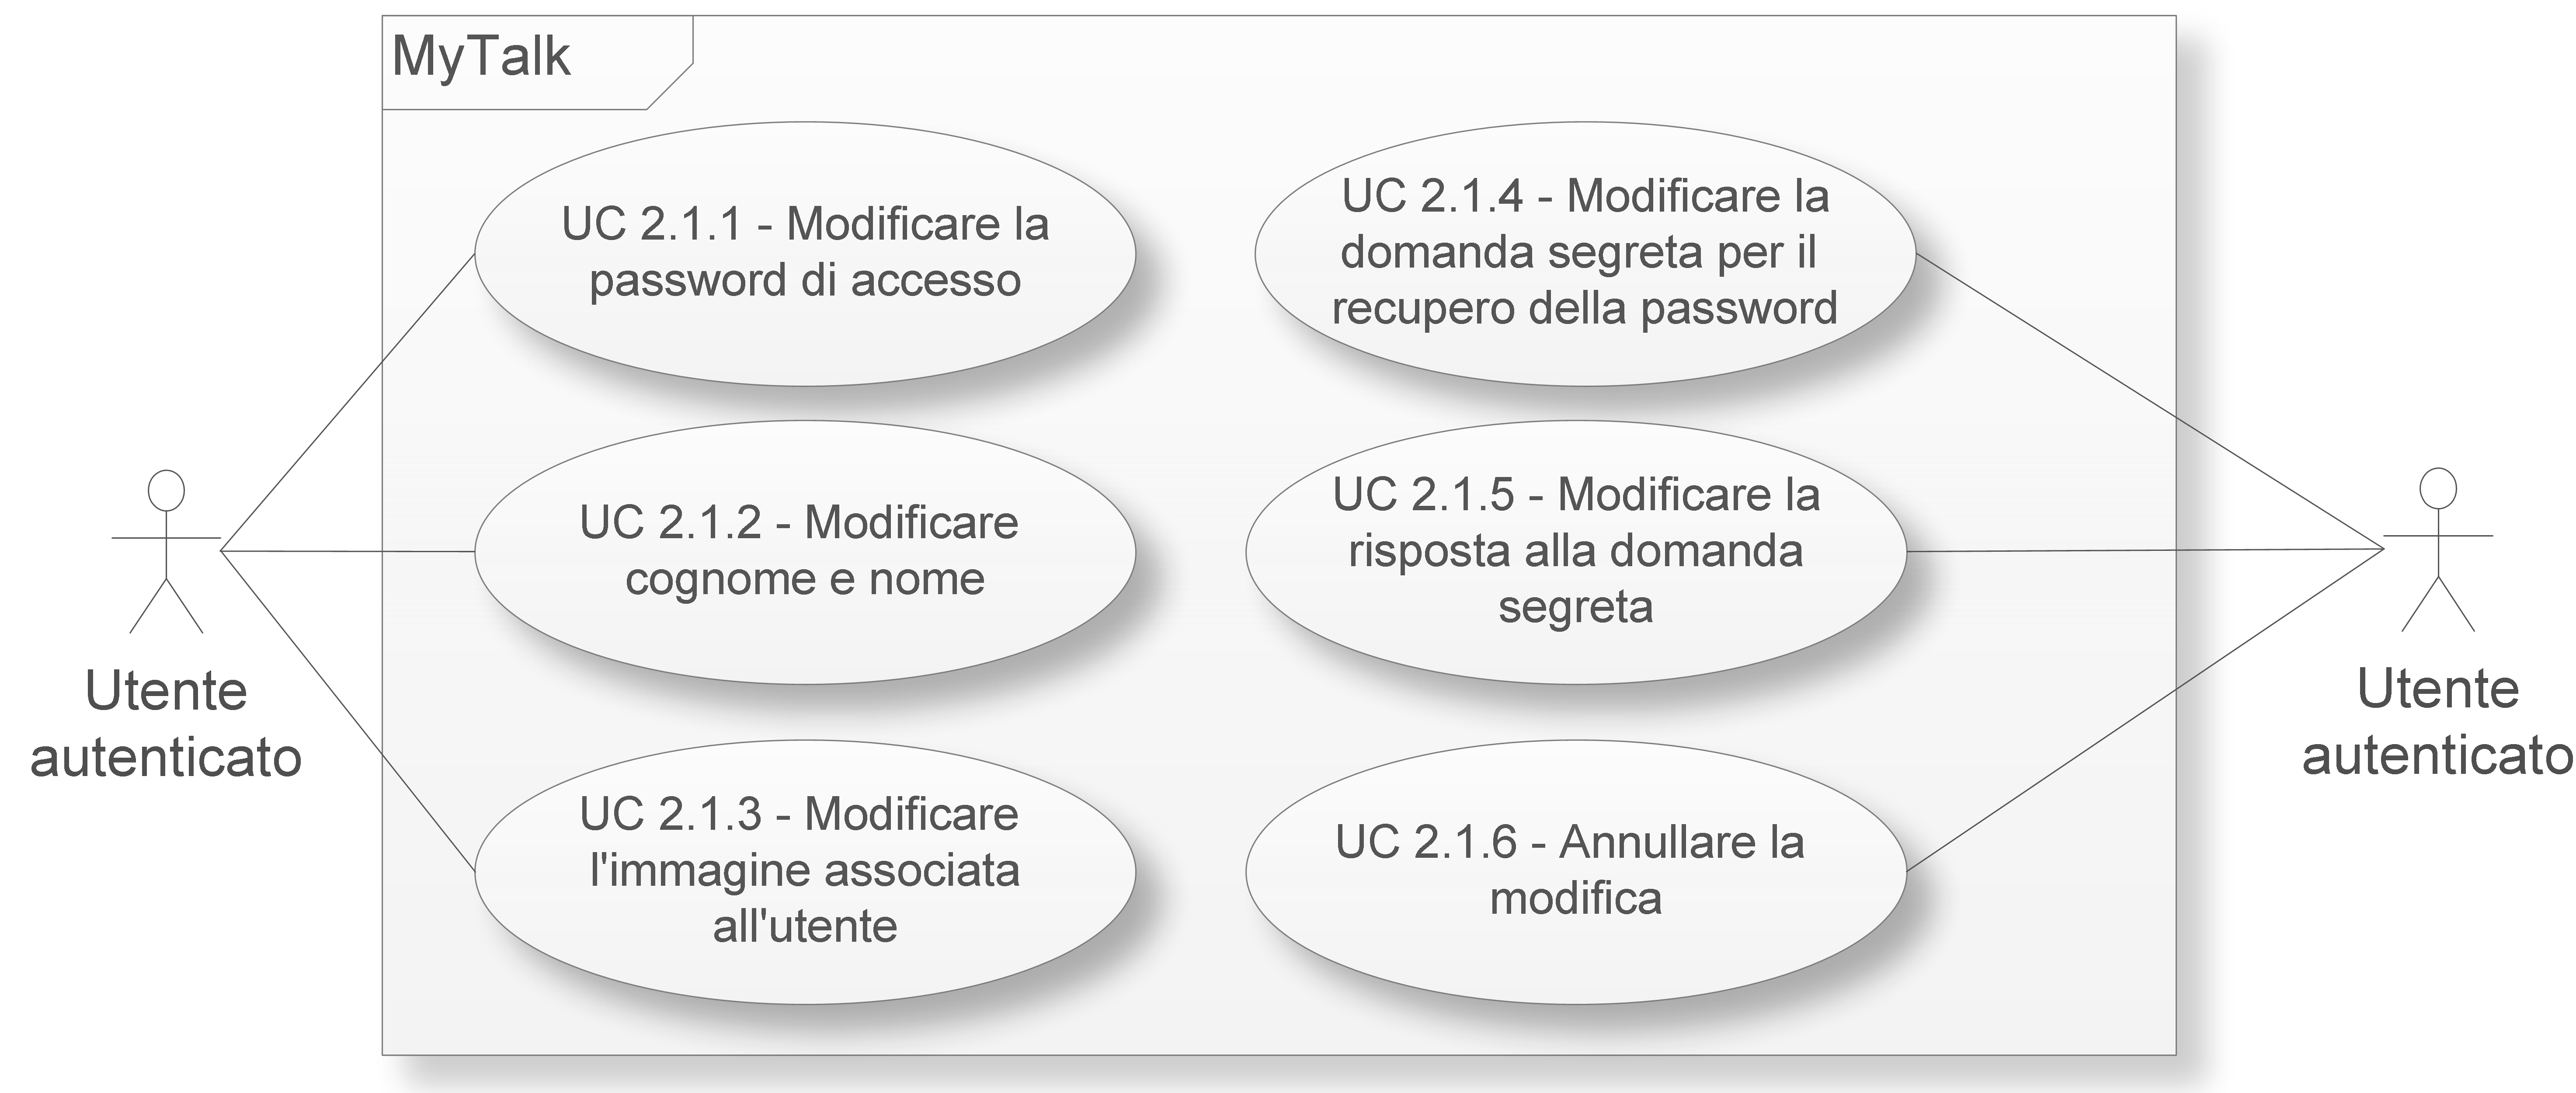
\includegraphics[width=.8\textwidth]{UC2-1}
\caption{}\label{fig:}
\end{center}
\end{figure}
\begin{description}
\item{\scshape\bfseries Attori principali:}Utente autenticato.
\item{\scshape\bfseries Scopo e descrizione:} un utente autenticato, ha la possibilità di modificare i propri dati personali, inseriti durante la sua registrazione, così da rimediare ad eventuali errori.
\item{\scshape\bfseries Precondizione:} l'utente corrente e' registrato nel sistema, ed ha effettuato il login.
\item{\scshape\bfseries Postcondizione:} i dati dell'utente sono stati aggiornati con i valori da lui inseriti.
\item{\scshape\bfseries Illustrazione scenario principale:} L'utente visualizza i valori correnti dei dati che lo riguardano e può apportare
le modifiche che ritiene necessarie. I dati che può modificare sono la password (UC2.1.1), il nome (UC2.1.2), il cognome (UC2.1.6), l'immagine profilo (UC2.1.3), la domanda segreta (UC2.1.4), la risposta alla domanda segreta (UC2.1.5). A questo punto può salvare le modifiche (UC2.1.8).
\item{\scshape\bfseries Illustrazione scenario alternativo:} Prima del salvataggio (UC2.1.8) l'utente può annullare l'operazione (UC2.1.7) tornando così alla schermata principale senza aver effettuato nessuna modifica.
\end{description}

\subsection{UC2.2: Gestire lo stato}
\begin{figure}[H]
\begin{center}
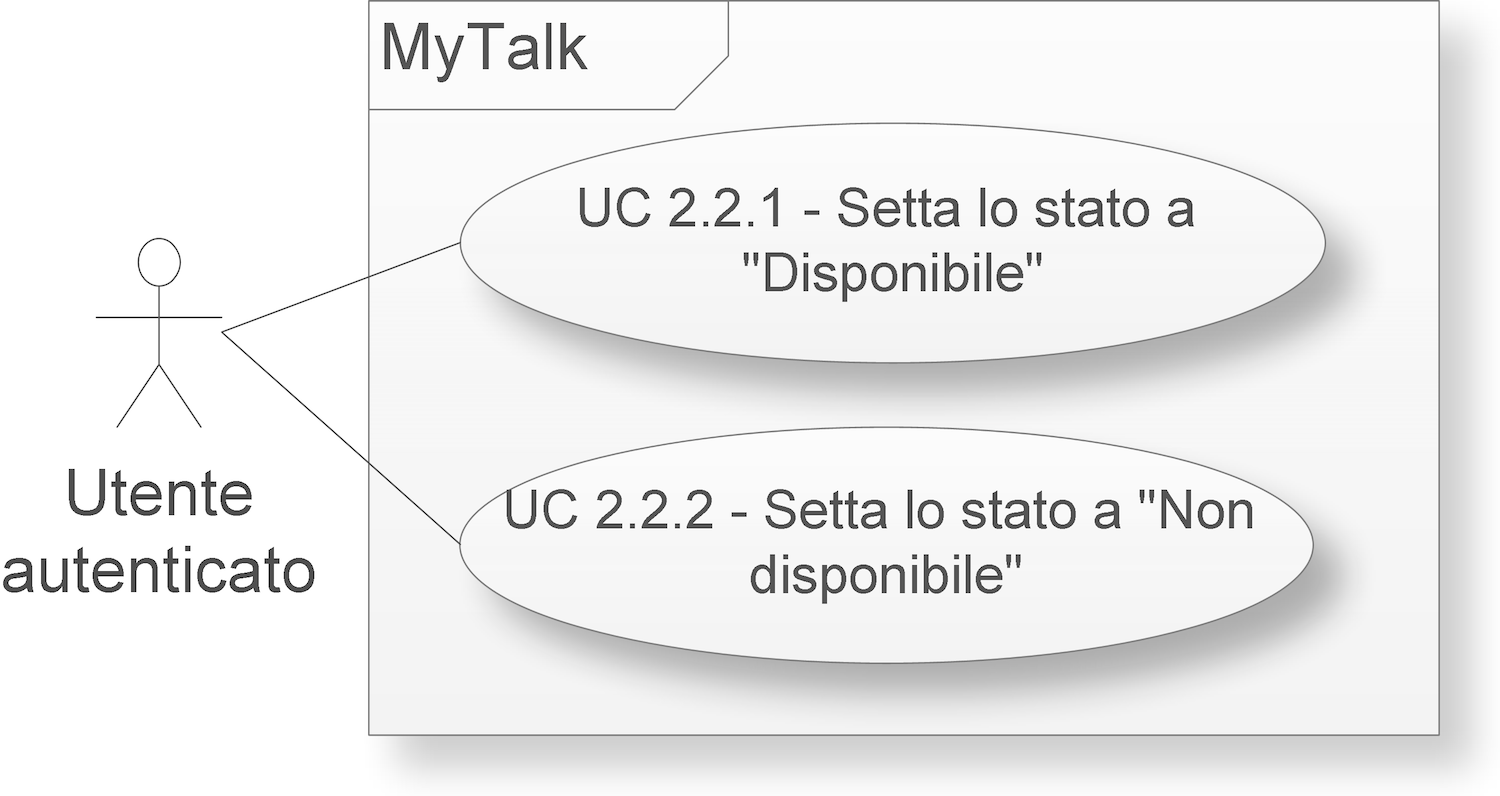
\includegraphics[width=.8\textwidth]{UC2-2}
\caption{}\label{fig:}
\end{center}
\end{figure}
\begin{description}
\item{\scshape\bfseries Attori principali:}Utente autenticato.
\item{\scshape\bfseries Scopo e descrizione:} L'utente potrà comunicare agli altri utenti la sua disponibilità o meno a comunicare, aggiornando il proprio stato.
\item{\scshape\bfseries Precondizione:} L'utente è registrato nel sistema ed ha eseguito l'accesso senza errori.
\item{\scshape\bfseries Postcondizione:} L'utente ha modificato il proprio stato.
\item{\scshape\bfseries Illustrazione scenario principale:} L'utente potrà scegliere di cambiare il proprio stato corrente. Gli stati tra cui può scegliere sono:disponibile (UC2.2.1)  e non disponibile (UC2.2.2).
\end{description}

\subsection{UC2.3: Gestione della rubrica}
\begin{figure}[H]
\begin{center}
\includegraphics[width=.8\textwidth]{UC2-3}
\caption{}\label{fig:}
\end{center}
\end{figure}
\begin{description}
\item{\scshape\bfseries Attori principali:}Utente autenticato.
\item{\scshape\bfseries Scopo e descrizione:} L'utente può visualizzare ed organizzare la rubrica dei propri contatti personali sulla base della lista degli utenti che si sono registrati, oppure importando i contati da un file esterno.
\item{\scshape\bfseries Precondizione:} L'utente ha effettuato la procedura di login ed è quindi autenticato.
\item{\scshape\bfseries Postcondizione:} Se l'utente ha attuato delle modifiche, queste sono state salvate. Altrimenti non ci sono state modifiche sui dati inerenti la rubrica.
\item{\scshape\bfseries Illustrazione scenario principale:} L'utente visualizza la propria rubrica divisa in gruppi. Può quindi scegliere una delle seguenti opzioni: aggiunge un contatto alla rubrica tramite ricerca (UC2.3.1), aggiunge un contatto in gruppi personalizzati (UC2.3.4), crea un nuovo gruppo (UC2.3.6); elimina un gruppo (UC2.3.8), aggiunge ed eliminare un contatto alla rubrica in un gruppo scelto tra quelli già creati (UC2.3.4 - UC2.3.5), elimina un contatto dalla propria rubrica (UC2.3.2), esporta i contatti presenti nella propria rubrica (UC2.3.9) e importa dei contatti prelevati da un file XML (UC2.3.10).
Inoltre potrà ordinare la rubrica in base a dei parametri (UC2.3.3).
\item{\scshape\bfseries Illustrazione scenario alternativo:} Se la ricerca del contatto da esito negativo viene riportato un errore (UC2.3.1.3).
\item{\scshape\bfseries Illustrazione scenario alternativo:} Se il contatto selezionato per l'inserimento nella rubrica, è già presente nella rubrica, allora compare un messaggio d'errore (UC2.3.1.3) che avvisa l'utente dell'impossibilità di aggiungere il contatto. (Non vengono visualizzati due errori separati ma un errore unico).
\end{description}

\subsection{UC2.4: Gestire segreteria personale}
\begin{figure}[H]
\begin{center}
\includegraphics[width=.8\textwidth]{UC2-4}
\caption{}\label{fig:}
\end{center}
\end{figure}
\begin{description}
\item{\scshape\bfseries Attori principali:}Utente autenticato.
\item{\scshape\bfseries Scopo e descrizione:} L'utente ha a disposizione una segreteria personale che può gestire.
\item{\scshape\bfseries Precondizione:} L'utente ha effettuato la procedura di login ed è quindi autenticato.
\item{\scshape\bfseries Postcondizione:} Il sistema ha eseguito con successo le operazioni richieste dall'utente.
\item{\scshape\bfseries Illustrazione scenario principale:} L'utente si trova nella sezione riguardante la segreteria e può ascoltare, se presenti, i messaggi lasciati dai propri contatti (UC2.4.1), cancellarle i messaggi ricevuti (UC2.4.2) ed infine cambiare lo stato del messaggio da letto a da leggere e viceversa.
\end{description}

\subsection{UC2.5.1: Connessione con altri utenti autenticati}
\begin{figure}[H]
\begin{center}
\includegraphics[width=.8\textwidth]{UC2-5-1}
\caption{}\label{fig:}
\end{center}
\end{figure}
\begin{description}
\item{\scshape\bfseries Attori principali:}Utente autenticato.
\item{\scshape\bfseries Scopo e descrizione:} Un utente, durante una chiamata audio, audio/video e chat, può eseguire diverse operazioni sulla connessione stabilita.
\item{\scshape\bfseries Precondizione:} L'utente è autenticato nel sistema, ed ha già stabilito una connessione con un utente autenticato.
\item{\scshape\bfseries Postcondizione:} L'utente ha concluso la comunicazione. La causa della terminazione può essere attribuita alla chiusura volontaria della connessione oppure al fatto che l'utente rimane l'unico attivo nella connessione.
\item{\scshape\bfseries Illustrazione scenario principale:} L'utente ha avviato una comunicazione. Mentre questa è in esecuzione, l'utente potrà: visualizzare le statistiche sulla comunicazione (UC2.5.1.1), condividere delle risorse dal proprio dispositivo (Condivisione di PDF, invio di file, condivisione di una lavagna grafica, e condivisione dello schermo)(UC2.5.1.2), visualizzare da quanto tempo è aperta la connessione (UC2.5.1.3), avviare e fermare una registrazione (UC2.5.1.6 - UC2.5.1.7), accettare o rifiutare una richiesta di registrazione inoltrata da un interlocutore (UC2.5.1.4 - UC2.5.1.5). Infine l'utente può decidere di terminare la comunicazione (UC2.5.1.8).
\end{description}

\subsection{UC2.5.1.1: Visualizzazione statistiche sulla comunicazione}
\begin{figure}[H]
\begin{center}
\includegraphics[width=.8\textwidth]{UC2-5-1-1}
\caption{}\label{fig:}
\end{center}
\end{figure}
\begin{description}
\item{\scshape\bfseries Attori principali:}Utente autenticato.
\item{\scshape\bfseries Scopo e descrizione:} L'utente visualizza i dettagli della comunicazione con un altro utente.
\item{\scshape\bfseries Precondizione:} L'utente sta comunicando con un altro utente del sistema.
\item{\scshape\bfseries Postcondizione:} L'utente ha visualizzato tutte le informazioni riguardanti la comunicazione.
\item{\scshape\bfseries Illustrazione scenario principale:} L'utente che comincia a comunicare con un altro utente ha a disposizione la visualizzazione di alcune informazioni sulla comunicazione in corso, come il numero di byte ricevuti ed inviati (UC2.5.1.1.1 - UC2.5.1.1.3), la latenza ossia il tempo che passa da quando un utente trasmette a quando l'altro utente riceve (UC2.5.1.1.5), la velocità di trasmissione dei dati (UC2.5.1.1.2) e i frame per secondo (fps) nel caso sia in corso una videochiamata (UC2.5.1.1.4).
\end{description}

\subsection{UC2.7: Ricerca di un utente}
\begin{figure}[H]
\begin{center}
\includegraphics[width=.8\textwidth]{UC2-7}
\caption{}\label{fig:}
\end{center}
\end{figure}
\begin{description}
\item{\scshape\bfseries Attori principali:}Utente autenticato.
\item{\scshape\bfseries Scopo e descrizione:} L'utente desidera ricercare altri utenti all'interno del sistema.
\item{\scshape\bfseries Precondizione:} L'utente è autenticato al sistema; la lista degli utenti registrati presso il server non è vuota.
\item{\scshape\bfseries Postcondizione:} L'utente ha ottenuto una lista (possibilmente vuota) di utenti che soddisfano i parametri di ricerca.
\item{\scshape\bfseries Illustrazione scenario principale:} Nel momento in cui un utente vuole ricercare un altro utente registrato nel sistema, ha la possibilità  di ricercarlo o nella propria rubrica (UC2.7.1) o nella lista di utenti registrati nel sistema (UC2.7.2).
\end{description}

\newpage\section{Requisiti di prodotto}
I requisiti verranno suddivisi in base alla loro priorità. Rispettivamente seguirà la lista dei requisiti obbligatori, facoltativi e desiferabili. Ogni requisito è identificato con il seguente formato RXYZI con:


		\begin{itemize}

			\item \textbf{X}: indica la tipologia dell'utente interessato dal requisito. I possibili valori che X può assumere sono U (utente) oppure S (sistema).

			\item \textbf{Y}: indica la tipologia del requisito, e può assumere i valori: F(funzionale), Q(qualitativo), P(prestazionale), D(dichiarativo).

			\item \textbf{Z}: indica il livello di priorità del requisito. Può assumere i valori O(obbligatorio), \\F(facoltativo), D(desiderabile).

			\item \textbf{I}: indica l'id numerico del requisito, denominato secondo le direttive delle norme di progetto.

		\end{itemize}


		Ogni requisito si può suddividere in sottorequisiti. Tale evento è evidenziato dal valore del campo I, come riportato nelle norme di progetto. Infine i requisiti sono ordinati (nelle proprie sezioni) in base all'ordine crescente del campo numerico I.\
Per quanto riguarda invece i requisiti di processo, si rimanda ai documenti \textit{piano\_di\_qualifica.2.0.pdf} (sez. 3.1) e \textit{norme\_di\_progetto.2.0.pdf} (in particolare le sez. 2, 3 e 4).

\subsection{Requisiti funzionali}


\subsubsection{Requisiti funzionali obbligatori}

\begin{center}
\rowcolors{2}{lightblue}{llightblue}\begin{longtable}{lp{.55\textwidth}l}
\toprule Codice & Requisito & Fonte\\
\midrule
RUFO1.0.0 & L'utente deve potersi autentificare nel server, così da permettere a quest'ultimo di rilevare la sua presenza nel sistema. & Interno \\
RSFO1.2.0 & Per effettuare il login è necessario inserire i dati utente & Interno\\
RSFO1.2.1 & Per effettuare il login è necessario inserire il proprio username & Interno\\
RSFO1.2.2 & Per effettuare il login è necessario inserire la propria password & Interno\\
RUFO2.0.0 & Registrazione del nuovo utente & Capitolato d'appalto \\
RSFO2.1.0 & Inserimento dei dati obbligatori per l’autenticazione & Interno \\
RSFO2.1.3 & Inserimento del campo obbligatorio username (e-mail) & Interno\\
RSFO2.1.4 & Inserimento del campo obbligatorio password & Interno\\
RSFO2.1.5 & Inserimento del campo obbligatorio ``domanda segreta'' & Interno\\
RSFO2.1.6 & Inserimento del campo obbligatorio ``risposta alla domanda segreta'' & Interno\\
RUFO5.0.0 & Possibilità di visualizzare la lista di utenti registrati nel sistema & Capitolato d'appalto \\
RUFO6.1.0 & stabilire una comunicazione audio con un utente in linea & Capitolato d'appalto \\
RUFO6.1.1 & Stabilire una comunicazione audio mediante inserimento d'indirizzo IP & Capitolato d'appalto \\
RUFO6.1.3 & Stabilire una comunicazione audio con un utente registrato e NON presente nella rubrica & Capitolato d'appalto \\
RUFO6.2.0 & Stabilire una comunicazione audio e video con un utente in linea & Capitolato d'appalto \\
RUFO6.2.1 & Stabilire una comunicazione audio e video mediante inserimento d'indirizzo IP & Capitolato d'appalto \\
RUFO6.2.3 & Stabilire una comunicazione audio e video con un utente registrato e NON presente nella rubrica & Capitolato d'appalto \\
RUFO6.4.0 & Mantenere la comunicazione audio e video fino a che uno dei due utenti non la chiude & Capitolato d'appalto \\
RUFO6.5.0 & Mantenere la comunicazione audio fino a che uno dei due utenti non la chiude & Capitolato d'appalto \\
RUFO7.0.0 & Indicare il tempo di comunicazione & Capitolato d'appalto \\
RUFO8.0.0 & Valutare il numero di byte trasmessi & Capitolato d'appalto \\
RUFO8.1.0 & Valutare il numero di byte inviati & Interno \\
RUFO8.2.0 & Valutare il numero di byte ricevuti & Interno \\
RUFO9.0.0 & Indicare la qualità della linea di trasmissione & Capitolato d'appalto \\
RUFO9.1.0 & Rilevare latenza & Capitolato d'appalto \\
RUFO9.2.0 & Rilevare velocità di trasmissione & Capitolato d'appalto \\
RSFO11.0.0 & Creare una connessione tra client, mediante l'utilizzo di un server & Capitolato d'appalto \\
RSFO11.1.0 & Utilizzo del protocollo webSocket per creare una connessione tra 2 utenti & Interno \\
RSFO12.0.0 & Gestire gli eventi dell'utente durante la connessione. & Interno \\
RUFO12.3.0 & Chi partecipa alla connessione può togliersi da essa & Interno \\
\bottomrule
\end{longtable}
\end{center}

\subsubsection{Requisiti funzionali desiderabili}

\begin{center}
\rowcolors{2}{lightblue}{llightblue}\begin{longtable}{lp{.55\textwidth}l}
\toprule Codice & Requisito & Fonte\\
\midrule
RUFD1.1.0 & Gestione password dimenticata & Interno \\
RUFD1.1.1 & Proporre la domanda segreta all'utente & Interno \\
RUFD1.1.2 & Invio di una mail all'utente contenete la password dimenticata & Interno \\
RSFD2.1.2 & Convalidare username (e-mail) dell'utente & Interno \\
RUFD12.2.0 & Chi crea la connessione può eliminare i membri del gruppo di chiamata & Interno \\
RUFD13.1.0 & Servizio chat tra 2 utenti & Interno \\
RSFD21.0.0 & Gestione interfaccia grafica in più lingue & Interno \\
\bottomrule
\end{longtable}
\end{center}

\subsubsection{Requisiti funzionali facoltativi}

\begin{center}
\rowcolors{2}{lightblue}{llightblue}\begin{longtable}{lp{.55\textwidth}l}
\toprule Codice & Requisito & Fonte\\
\midrule
RUFF3.0.0 & Modifica dati utente & Interno \\
RUFF3.1.0 & Modifica dei dati per l'autenticazione & Interno \\
RUFF3.1.1 & Modifica della password & Interno\\
RUFF3.1.2 & Modifica della ``domanda segreta'' & Interno\\
RUFF3.1.3 & Modifica della ``risposta alla domanda segreta'' & Interno\\
RUFF3.2.0 & Modifica dei dati anagrafici facoltativi & Interno \\
RUFF3.2.1 & Modifica del nome & Interno\\
RUFF3.2.2 & Modifica del cognome & Interno\\
RUFF3.2.3 & Modifica dell'immagine profilo & Interno\\
RUFF4.0.0 & L'utente ha a disposizione una rubrica personale & Interno \\
RUFF4.1.0 & Possibilità d'inserire utenti nella propria rubrica & Capitolato d'appalto \\
RUFF4.2.0 & Possibilità di eliminare un utente dalla propria rubrica & Interno \\
RUFF4.3.0 & Possibilità di ordinare la rubrica su alcuni parametri rilevanti & Interno \\
RUFF4.3.1 & Possibilità di ordinare la rubrica in relazione al nome utente & Interno\\
RUFF4.3.2 & Possibilità di ordinare la rubrica in relazione al nome dei gruppi & Interno\\
RUFF4.4.0 & Possibilità di suddividere la rubrica in gruppi & Interno \\
RUFF4.4.1 & Possibilità di togliere un elemento da un gruppo & Interno \\
RUFF4.4.2 & Possibilità di aggiungere un elemento in un gruppo & Interno \\
RUFF4.4.3 & Possibilità di creare un gruppo & Interno \\
RUFF4.4.4 & Possibilità di eliminare un gruppo & Interno \\
RUFF4.5.0 & Possibilità di esportare in xml la rubrica personale & Interno \\
RUFF4.6.0 & Possibilità di modificare la rubrica importando un file xml & Interno \\
RUFF4.7.0 & Ricerca di un utente nella propria rubrica. & Interno \\
RUFF4.7.1 & Ricerca degli utenti nel cui nome compare la parola ricercata & Interno\\
RUFF4.7.2 & Ricerca degli utenti nel cui cognome compare la parola ricercata & Interno\\
RUFF4.7.3 & Ricerca degli utenti appartenenti ad un gruppo nel cui nome compare la parola ricercata & Interno\\
RUFF5.1.0 & Possibilità di cercare un utente dalla lista & Interno \\
RUFF5.1.1 & Possibilità di cercare un utente dalla lista, in relazione al nome utente & Interno\\
RUFF5.1.2 & Possibilità di cercare un utente dalla lista, in relazione al email & Interno\\
RUFF6.1.2 & Stabilire una comunicazione audio con un utente registrato e presente nella rubrica & Capitolato d'appalto \\
RUFF6.1.4 & Promuovere una comunicazione audio avviata con un utente in una comunicazione audio e video & Interno \\
RUFF6.2.2 & Stabilire una comunicazione audio e video con un utente presente nella rubrica & Capitolato d'appalto \\
RUFF6.2.4 & Declassare una comunicazione audio e video avviata con un utente in una comunicazione solo audio & Interno \\
RUFF6.2.5 & Disattivare la webcam utente pur continuando a ricevere il segnale video proveniente dall'altro capo della comunicazione & Interno \\
RUFF6.3.0 & Disattivare il microfono utente pur continuando a ricevere il segnale video proveniente dall'altro capo della comunicazione & Interno \\
RUFF9.3.0 & Rilevazione frame per secondo & Interno \\
RSFF11.2.0 & Utilizzo del protocollo webSocket per creare una connessione tra più di 2 utenti & Interno \\
RSFF12.1.0 & Estendere la connessione ad altri client & Interno \\
RUFF13.0.0 & Servizio chat testuale & Capitolato d'appalto \\
RUFF13.2.0 & Servizio chat tra più di 2 utenti & Interno \\
RUFF14.0.0 & Registrazione della chiamata & Capitolato d'appalto \\
RUFF14.1.0 & Necessità di autorizzazione dagli utenti della chiamata per poter avviare la registrazione & Interno \\
RUFF14.2.0 & Registrazione audio & Interno \\
RUFF14.3.0 & Possibilità di riascoltare la registrazione & Interno \\
RUFF15.0.0 & L'utente avrà a disposizione una segreteria telefonica. & Interno \\
RUFF15.1.0 & Possibilità di lasciare un audio messaggio in segreteria & Interno \\
RUFF15.2.0 & Possibilità di lasciare un audio e video messaggio in segreteria & Capitolato d'appalto \\
RUFF15.3.0 & Possibilità di ascoltare la propria segreteria & Interno \\
RUFF15.4.0 & Possibilità di cancellare messaggi della segretaria & Interno \\
RUFF15.5.0 & Possibilità di cambiare lo stato del messaggio da "non ascoltato" a "ascoltato" & Interno \\
RUFF16.0.0 & Fornire la possibilità di cambiare lo stato utente & Interno \\
RUFF16.1.0  & Fornire la possibilità di impostare 'disponibile' come stato utente & Interno \\
RUFF16.2.0 & Fornire la possibilità di impostare 'non disponibile' come stato utente & Interno \\
RUFF17.0.0 & Dare la possibilità di vedere gli stati personali altrui. & Interno \\
RUFF18.0.0 & Presenza di una Blacklist & Interno \\
RUFF19.0.0 & Presenza di uno storico delle chiamate & Interno \\
RUFF20.0.0 & Condividere risorse & Interno \\
RUFF20.1.0 & Condivisione del monitor & Interno \\
RUFF20.2.0 & Condivisione pdf & Interno \\
RUFF20.3.0 & Condivisione lavagna grafica. & Interno \\
RUFF20.4.0 & Invio file & Interno \\
\bottomrule
\end{longtable}
\end{center}

\subsection{Requisiti qualitativi}

\subsubsection{Requisiti qualitativi obbligatori}

\begin{center}
\rowcolors{2}{lightblue}{llightblue}\begin{longtable}{lp{.55\textwidth}l}
\toprule Codice & Requisito & Fonte\\
\midrule
RSQO6.4.0 & L'applicativo dev'essere predisposto a facili modifiche dettate da evoluzioni future di WebRTC. & Capitolato d'appalto \\
\bottomrule
\end{longtable}
\end{center}

\begin{center}
\rowcolors{2}{lightblue}{llightblue}\begin{longtable}{lp{.55\textwidth}l}
\toprule Codice & Requisito & Fonte\\
\midrule
RSQF23.0.0 & Verificare che l'applicativo funzioni anche sotto gli altri browser del S.O. Windows & Interno \\
RSQF23.1.0 & Verificare che funzioni con Opera (versione 12.0 minima) & Capitolato d'appalto \\
RSQF23.2.0 & Verificare che funzioni con Firefox (versione 17.0 minima) & Capitolato d'appalto \\
RSQF23.3.0 & Verificare che funzioni con Internet Explorer (versione 10.0 minima) & Capitolato d'appalto \\
RSQF23.4.0 & Verificare che funzioni con Safari (versione 6.0 minima) & Capitolato d'appalto \\
RSQF24.0.0 & Verificare che l'applicativo funzioni anche sotto gli altri browser del S.O. Linux & Interno \\
RSQF24.1.0 & Verificare che funzioni con Opera (versione 12.0 minima) & Capitolato d'appalto \\
RSQF24.2.0 & Verificare che funzioni con Firefox (versione 17.0 minima) & Capitolato d'appalto \\
RSQF24.3.0 & Verificare che funzioni con Chromium (versione 25.0.1313 minima) & Interno \\
RSQF25.0.0 & Verificare che l'applicativo funzioni anche sotto gli altri browser del S.O. Macintosh & Interno \\
RSQF25.1.0 & Verificare che funzioni con Opera (versione 12.0 minima) & Capitolato d'appalto \\
RSQF25.2.0 & Verificare che funzioni con Firefox (versione 17.0 minima) & Capitolato d'appalto \\
RSQF25.3.0 & Verificare che funzioni con Safari  (versione 6.0 minima) & Capitolato d'appalto \\
RSQF26.0.0 & Il software dovrà essere compatibile con componenti realizzati in Flash & Capitolato d'appalto \\
\bottomrule
\end{longtable}
\end{center}

\subsection{Requisiti dichiarativi}

\subsubsection{Requisiti dichiarativi obbligatori}

\begin{center}
\rowcolors{2}{lightblue}{llightblue}\begin{longtable}{lp{.55\textwidth}l}
\toprule Codice & Requisito & Fonte\\
\midrule
RSDO6.0.0 & Gestire le comunicazioni utente tramite WebRTC & Capitolato d'appalto \\
RSDO10.0.0 & L'intero sistema deve essere contenuto in un unica pagina Web & Capitolato d'appalto \\
RSDO10.1.0 & L'interfaccia grafica non deve subire refresh per ogni operazione dell'utente & Interno \\
RSDO11.3.0 & Il server sarà implementato tramite il linguaggio Java. & Capitolato d'appalto \\
RSDO11.4.0 & Il server sarà coinvolto solo per avviare la comunicazione & Capitolato d'appalto \\
RSDO22.0.0 & L'applicativo deve essere fruibile attraverso un browser web & Capitolato d'appalto \\
RSDO22.1.0 & L'applicativo web deve funzionare nel browser web Google Chrome (versione minima 23.0.1271.97m) & Capitolato d'appalto \\
\bottomrule
\end{longtable}
\end{center}

\subsubsection{Requisiti dichiarativi desiderabili}

\begin{center}
\rowcolors{2}{lightblue}{llightblue}\begin{longtable}{lp{.55\textwidth}l}
\toprule Codice & Requisito & Fonte\\
\midrule
RSDD2.1.1 & L'utente ha una stima per la complessità della propria password & Interno \\
RSDD2.2.0 & Inserimento dei dati facoltativi riferiti all'anagrafica & Interno \\
\bottomrule
\end{longtable}
\end{center}

\begin{center}
\rowcolors{2}{lightblue}{llightblue}\begin{longtable}{lp{.55\textwidth}l}
\toprule Codice & Requisito & Fonte\\
\midrule
\bottomrule
\end{longtable}
\end{center}

\newpage
\section{Requisiti di qualità di processo}\label{sec:qualitaProcesso}

Al fine di introdurre qualità nei processi implementati per la creazione del prodotto, il team ha ritenuto necessario identificare dei requisiti da tenere in considerazione nelle scelta delle attività e nella loro pianificazione. Per la loro peculiarità e la sostanziale separazione dai requisiti di prodotto, i requisiti di processo sono stati riportati in una sezione separata da quest'ultimi. Di seguito è riportata la tabella dei requisiti evidenziati.

Il sistema di nominazione è analogo a quello usato nei ``Requisiti di prodotto'' e nello specifico tali requisiti saranno identificati come RSQO (requisiti obbligatori di qualità di sistema).

\begin{center}
\rowcolors{2}{lightblue}{llightblue}\begin{longtable}{lp{.55\textwidth}l}
\toprule Codice & Requisito & Fonte\\
\midrule
RSQO27.0.0 & il modello SPY e CMMI sono utilizzati per valutare la qualità dei processi & Interno \\
RSQO28.0.0 & Gli standard di qualità hanno come riferimento lo standard ISO/9126:2001 & Interno \\
RSQO28.1.0 & Adozione del ciclo di Deming (PDCA) per valutare e migliorare i processi & Interno \\
RSQO29.0.0 & Distinte modalità di verifica per ogni attività durante il ciclo di vita progettuale & Interno \\
RSQO29.1.0 & Modalità di verifica specifiche per l'analisi dei requisiti & Interno \\
RSQO29.2.0 & Modalità di verifica specifiche per la progettazione di alto livello & Interno \\
RSQO29.3.0 & Modalità di verifica specifiche per la progettazione di dettaglio & Interno \\
RSQO29.4.0 & Modalità di verifica specifiche per la codifica & Interno \\
RSQO29.4.1 & Utilizzo di metriche specifiche per valutare il codice & Interno \\
RSQO29.5.0 & Modalità di verifica specifiche per validazione & Interno \\
RSQO30.0.0 & Uso di un sistema di ticketing (tracciato) per evidenziare e risolvere errori o problematiche & Interno \\
RSQO31.0.0 & l'attività di progettazione condotta nel rispetto dei principi della programmazione ad oggetti & Interno \\
RSQO31.1.0 & durante la progettazione è imposto l'utilizzo di interfacce & Interno \\
RSQO31.2.0 & il processo di individuazione delle classi e il loro corrispettivo inserimento in una componente è giustificato dal significato e dall'utilizzo della classe stessa (principio di coesione) & Interno \\
\bottomrule
\end{longtable}
\end{center}

\newpage\section{Tracciamento use case - requisiti}\label{sec:tracciamento}

\begin{center}
\rowcolors{2}{lightblue}{llightblue}\begin{longtable}{lp{.55\textwidth}l}
\toprule Codice UC & Nome UC  & Requisito\\
\midrule
UC1 & Login e registrazione & RUFO1.0.0 \\
 &  & RUFD1.1.0 \\
 &  & RUFD1.1.1 \\
 &  & RUFD1.1.2 \\
 &  & RSFO1.2.0 \\
 &  & RSFO1.2.1 \\
 &  & RSFO1.2.2 \\
 &  & RUFO2.0.0 \\
 &  & RSFO2.1.0 \\
 &  & RSDD2.1.1 \\
 &  & RSFO2.1.3 \\
 &  & RSFO2.1.4 \\
 &  & RSFO2.1.5 \\
 &  & RSFO2.1.6 \\
 &  & RSFD2.1.2 \\
 &  & RSDD2.2.0 \\
UC2 & Home screen dell'applicativo & RUFF3.0.0 \\
 &  & RUFF3.1.0 \\
 &  & RUFF3.1.1 \\
 &  & RUFF3.1.2 \\
 &  & RUFF3.1.3 \\
 &  & RUFF3.2.1 \\
 &  & RUFF3.2.2 \\
 &  & RUFF3.2.3 \\
 &  & RUFF3.2.0 \\
 &  & RUFF4.0.0 \\
 &  & RUFF4.1.0 \\
 &  & RUFF4.2.0 \\
 &  & RUFF4.3.0 \\
 &  & RUFF4.3.1 \\
 &  & RUFF4.3.2 \\
 &  & RUFF4.4.0 \\
 &  & RUFF4.4.1 \\
 &  & RUFF4.4.2 \\
 &  & RUFF4.4.3 \\
 &  & RUFF4.4.4 \\
 &  & RUFF4.5.0 \\
 &  & RUFF4.6.0 \\
 &  & RUFF4.7.0 \\
 &  & RUFF4.7.1 \\
 &  & RUFF4.7.2 \\
 &  & RUFF4.7.3 \\
 &  & RUFO5.0.0 \\
 &  & RUFF5.1.0 \\
 &  & RUFF5.1.1 \\
 &  & RUFF5.1.2 \\
 &  & RUFO6.1.0 \\
 &  & RUFO6.1.1 \\
 &  & RUFF6.1.2 \\
 &  & RUFO6.1.3 \\
 &  & RUFF6.1.4 \\
 &  & RUFO6.2.0 \\
 &  & RUFO6.2.1 \\
 &  & RUFF6.2.2 \\
 &  & RUFO6.2.3 \\
 &  & RUFF6.2.4 \\
 &  & RUFF6.2.5 \\
 &  & RUFF6.3.0 \\
 &  & RUFO7.0.0 \\
 &  & RUFO8.0.0 \\
 &  & RUFO8.1.0 \\
 &  & RUFO8.2.0 \\
 &  & RUFO9.0.0 \\
 &  & RUFO9.1.0 \\
 &  & RUFO9.2.0 \\
 &  & RUFF9.3.0 \\
 &  & RSFF12.1.0 \\
 &  & RUFD12.2.0 \\
 &  & RUFO12.3.0 \\
 &  & RUFF13.0.0 \\
 &  & RUFD13.1.0 \\
 &  & RUFF13.2.0 \\
 &  & RUFF14.0.0 \\
 &  & RUFF14.1.0 \\
 &  & RUFF14.2.0 \\
 &  & RUFF15.0.0 \\
 &  & RUFF15.1.0 \\
 &  & RUFF15.2.0 \\
 &  & RUFF15.3.0 \\
 &  & RUFF15.4.0 \\
 &  & RUFF15.5.0 \\
 &  & RUFF16.0.0 \\
 &  & RUFF17.0.0 \\
 &  & RUFF18.0.0 \\
 &  & RUFF19.0.0 \\
 &  & RUFF20.0.0 \\
 &  & RUFF20.1.0 \\
 &  & RUFF20.2.0 \\
 &  & RUFF20.3.0 \\
 &  & RUFF20.4.0 \\
UC1.1 & Login utente & RUFO1.0.0 \\
 &  & RSFO1.2.0 \\
UC1.2 & Registrazione & RUFO2.0.0 \\
 &  & RSFO2.1.0 \\
 &  & RSDD2.1.1 \\
 &  & RSFD2.1.2 \\
 &  & RSFO2.1.3 \\
 &  & RSFO2.1.4 \\
 &  & RSFO2.1.5 \\
 &  & RSFO2.1.6 \\    
 &  & RSDD2.2.0 \\
UC1.3 & Recupero della password & RUFD1.1.0 \\
 &  & RUFD1.1.1 \\
 &  & RUFD1.1.2 \\
UC2.1 & Gestione account & RUFF3.0.0 \\
 &  & RUFF3.1.0 \\
 &  & RUFF3.1.1 \\
 &  & RUFF3.1.2 \\
 &  & RUFF3.1.3 \\
 &  & RUFF3.2.0 \\
UC2.2 & Gestire lo stato & RUFF16.0.0 \\
UC2.3 & Gestione della rubrica & RUFF4.0.0 \\
 &  & RUFF4.1.0 \\
 &  & RUFF4.2.0 \\
 &  & RUFF4.3.0 \\
 &  & RUFF4.3.1 \\
 &  & RUFF4.3.2 \\
 &  & RUFF4.4.0 \\
 &  & RUFF4.4.1 \\
 &  & RUFF4.4.2 \\
 &  & RUFF4.4.3 \\
 &  & RUFF4.4.4 \\
 &  & RUFF4.5.0 \\
 &  & RUFF4.6.0 \\
 &  & RUFF4.7.0 \\
 &  & RUFF4.7.1 \\
 &  & RUFF4.7.2 \\
 &  & RUFF4.7.3 \\
 &  & RUFO5.0.0 \\
 &  & RUFF5.1.0 \\
 &  & RUFF5.1.1 \\
 &  & RUFF5.1.2 \\
 &  & RUFF18.0.0 \\
UC2.4 & Gestire segreteria personale & RUFF15.0.0 \\
 &  & RUFF15.1.0 \\
 &  & RUFF15.2.0 \\
 &  & RUFF15.3.0 \\
 &  & RUFF15.4.0 \\
 &  & RUFF15.5.0 \\
UC2.7 & Ricerca di un utente & RUFF4.7.0 \\
 &  & RUFF4.7.1 \\
 &  & RUFF4.7.2 \\
 &  & RUFF4.7.3 \\
 &  & RUFF5.1.0 \\
 &  & RUFF5.1.1 \\
 &  & RUFF5.1.2 \\
UC2.5.1 & Connessione con altri utenti autenticati & RUFO6.1.0 \\
 &  & RUFO6.1.1 \\
 &  & RUFF6.1.2 \\
 &  & RUFO6.1.3 \\
 &  & RUFF6.1.4 \\
 &  & RUFO6.2.0 \\
 &  & RUFO6.2.1 \\
 &  & RUFF6.2.2 \\
 &  & RUFO6.2.3 \\
 &  & RUFF6.2.4 \\
 &  & RUFF6.2.5 \\
 &  & RUFF6.3.0 \\
 &  & RUFO7.0.0 \\
 &  & RUFO8.0.0 \\
 &  & RUFO8.1.0 \\
 &  & RUFO8.2.0 \\
 &  & RUFO9.0.0 \\
 &  & RUFO9.1.0 \\
 &  & RUFO9.2.0 \\
 &  & RUFF9.3.0 \\
 &  & RSFO12.0.0 \\
 &  & RSFF12.1.0 \\
 &  & RUFD12.2.0 \\
 &  & RUFO12.3.0 \\
 &  & RUFF13.0.0 \\
 &  & RUFD13.1.0 \\
 &  & RUFF13.2.0 \\
 &  & RUFF14.0.0 \\
 &  & RUFF14.1.0 \\
 &  & RUFF14.2.0 \\
 &  & RUFF20.0.0 \\
 &  & RUFF20.1.0 \\
 &  & RUFF20.2.0 \\
 &  & RUFF20.3.0 \\
 &  & RUFF20.4.0 \\
UC2.5.1.1 & Visualizzazione statistiche sulla comunicazione & RUFO7.0.0 \\
 &  & RUFO8.0.0 \\
 &  & RUFO8.1.0 \\
 &  & RUFO8.2.0 \\
 &  & RUFO9.0.0 \\
 &  & RUFO9.1.0 \\
 &  & RUFO9.2.0 \\
 &  & RUFF9.3.0 \\
\bottomrule
\end{longtable}
\end{center}
\newpage\section{Tracciamento requisiti - use case}\label{sec:tracciamento}

\begin{center}
\rowcolors{2}{lightblue}{llightblue}\begin{longtable}{lp{.55\textwidth}l}
\toprule Requisito & Codice UC\\
\midrule
RUFO1.0.0 & UC1 \\
 & UC1.1 \\
RUFD1.1.0 & UC1 \\
 & UC1.3 \\
RUFD1.1.1 & UC1 \\
 & UC1.3 \\
RUFD1.1.2 & UC1 \\
 & UC1.3 \\
RSFO1.2.0 & UC1 \\
 & UC1.1 \\
RSFO1.2.1 & UC1 \\
 & UC1.1 \\
RSFO1.2.2 & UC1 \\
 & UC1.1 \\ 
RUFO2.0.0 & UC1 \\
 & UC1.2 \\
RSFO2.1.0 & UC1 \\
 & UC1.2 \\
RSDD2.1.1 & UC1 \\
 & UC1.2 \\
RSFD2.1.2 & UC1 \\
 & UC1.2 \\
RSFO2.1.3 & UC1\\
 & UC2\\
RSFO2.1.4 & UC1\\
 & UC2\\
RSFO2.1.5 & UC1\\
 & UC2\\
RSFO2.1.6 & UC1\\
 & UC2\\
RSDD2.2.0 & UC1 \\
 & UC1.2 \\
RUFF3.0.0 & UC2 \\
 & UC2.1 \\
RUFF3.1.0 & UC2 \\
 & UC2.1 \\
RUFF3.1.1 & UC2 \\
 & UC2.1 \\
RUFF3.1.2 & UC2 \\
 & UC2.1 \\
RUFF3.1.3 & UC2 \\
 & UC2.1 \\
RUFF3.2.0 & UC2 \\
 & UC2.1 \\
RUFF3.2.1 & UC2 \\
 & UC2.1 \\
RUFF3.2.2 & UC2 \\
 & UC2.1 \\
RUFF3.2.3 & UC2 \\
 & UC2.1 \\
RUFF4.0.0 & UC2 \\
 & UC2.3 \\
RUFF4.1.0 & UC2 \\
 & UC2.3 \\
RUFF4.2.0 & UC2 \\
 & UC2.3 \\
RUFF4.3.0 & UC2 \\
 & UC2.3 \\
RUFF4.3.1 & UC2 \\
 & UC2.3 \\
RUFF4.3.2 & UC2 \\
 & UC2.3 \\
RUFF4.4.0 & UC2 \\
 & UC2.3 \\
RUFF4.4.1 & UC2 \\
 & UC2.3 \\
RUFF4.4.2 & UC2 \\
 & UC2.3 \\
RUFF4.4.3 & UC2 \\
 & UC2.3 \\
RUFF4.4.4 & UC2 \\
 & UC2.3 \\
RUFF4.5.0 & UC2 \\
 & UC2.3 \\
RUFF4.6.0 & UC2 \\
 & UC2.3 \\
RUFF4.7.0 & UC2 \\
 & UC2.3 \\
 & UC2.7 \\
RUFF4.7.1 & UC2 \\
 & UC2.3 \\
 & UC2.7 \\
RUFF4.7.2 & UC2 \\
 & UC2.3 \\
 & UC2.7 \\
RUFF4.7.3 & UC2 \\
 & UC2.3 \\
 & UC2.7 \\
RUFO5.0.0 & UC2 \\
 & UC2.3 \\
RUFF5.1.0 & UC2 \\
 & UC2.3 \\
 & UC2.7 \\
RUFF5.1.1 & UC2 \\
 & UC2.3 \\
 & UC2.7 \\
RUFF5.1.2 & UC2 \\
 & UC2.3 \\
 & UC2.7 \\
RUFO6.1.0 & UC2 \\
 & UC2.5.1 \\
RUFO6.1.1 & UC2 \\
 & UC2.5.1 \\
RUFF6.1.2 & UC2 \\
 & UC2.5.1 \\
RUFO6.1.3 & UC2 \\
 & UC2.5.1 \\
RUFF6.1.4 & UC2 \\
 & UC2.5.1 \\
RUFO6.2.0 & UC2 \\
 & UC2.5.1 \\
RUFO6.2.1 & UC2 \\
 & UC2.5.1 \\
RUFF6.2.2 & UC2 \\
 & UC2.5.1 \\
RUFO6.2.3 & UC2 \\
 & UC2.5.1 \\
RUFF6.2.4 & UC2 \\
 & UC2.5.1 \\
RUFF6.2.5 & UC2 \\
 & UC2.5.1 \\
RUFF6.3.0 & UC2 \\
 & UC2.5.1 \\
RUFO7.0.0 & UC2 \\
 & UC2.5.1 \\
 & UC2.5.1.1 \\
RUFO8.0.0 & UC2 \\
 & UC2.5.1 \\
 & UC2.5.1.1 \\
RUFO8.1.0 & UC2 \\
 & UC2.5.1 \\
 & UC2.5.1.1 \\
RUFO8.2.0 & UC2 \\
 & UC2.5.1 \\
 & UC2.5.1.1 \\
RUFO9.0.0 & UC2 \\
 & UC2.5.1 \\
 & UC2.5.1.1 \\
RUFO9.1.0 & UC2 \\
 & UC2.5.1 \\
 & UC2.5.1.1 \\
RUFO9.2.0 & UC2 \\
 & UC2.5.1 \\
 & UC2.5.1.1 \\
RUFF9.3.0 & UC2 \\
 & UC2.5.1 \\
 & UC2.5.1.1 \\
RSFO12.0.0 & UC2.5.1 \\
RSFF12.1.0 & UC2 \\
 & UC2.5.1 \\
RUFD12.2.0 & UC2 \\
 & UC2.5.1 \\
RUFO12.3.0 & UC2 \\
 & UC2.5.1 \\
RUFF13.0.0 & UC2 \\
 & UC2.5.1 \\
RUFD13.1.0 & UC2 \\
 & UC2.5.1 \\
RUFF13.2.0 & UC2 \\
 & UC2.5.1 \\
RUFF14.0.0 & UC2 \\
 & UC2.5.1 \\
RUFF14.1.0 & UC2 \\
 & UC2.5.1 \\
RUFF14.2.0 & UC2 \\
 & UC2.5.1 \\
RUFF15.0.0 & UC2 \\
 & UC2.4 \\
RUFF15.1.0 & UC2 \\
 & UC2.4 \\
RUFF15.2.0 & UC2 \\
 & UC2.4 \\
RUFF15.3.0 & UC2 \\
 & UC2.4 \\
RUFF15.4.0 & UC2 \\
 & UC2.4 \\
RUFF15.5.0 & UC2 \\
 & UC2.4 \\
RUFF16.0.0 & UC2 \\
 & UC2.2 \\
RUFF17.0.0 & UC2 \\
RUFF18.0.0 & UC2 \\
 & UC2.3 \\
RUFF19.0.0 & UC2 \\
RUFF20.0.0 & UC2 \\
 & UC2.5.1 \\
RUFF20.1.0 & UC2 \\
 & UC2.5.1 \\
RUFF20.2.0 & UC2 \\
 & UC2.5.1 \\
RUFF20.3.0 & UC2 \\
 & UC2.5.1 \\
RUFF20.4.0 & UC2 \\
 & UC2.5.1 \\
\bottomrule
\end{longtable}
\end{center}


\end{document}
